\chapter[The ionization of metal-rich absorbers in a $z=2.92$ radio galaxy halo]{MUSE unravels the ionization and origin of metal enriched absorbers in the gas halo of a $z = 2.92$ radio galaxy }

{\it Published in Astronomy \& Astrophysics, Volume 625, A102, 20 pp.\\
Authors: {\bf S. Kolwa},
J. Vernet,
C. De Breuck,
M. Villar-Martin,
A. Humphrey,
F. Arrigoni-Battaia,
B. Gullberg,
T. Falkendal,
G. Drouart,
M. Lehnert,
D. Wylezalek, and 
A. Man}    \\

\section*{Abstract}
We have used the Multi-Unit Spectroscopic Explorer (MUSE) to study the circumgalactic medium (CGM) of a $z = 2.92$ radio galaxy, MRC 0943-242, by parametrising its emitting and absorbing gas. In both \lya~$\lam$1216 and \ion{He}{II} $\lam$1640 lines, we observe emission with velocity shifts of $\Delta \varv \simeq-1000$ km s$^{-1}$ from the systemic redshift of the galaxy. These blueshifted components represent kinematically perturbed gas that is aligned with the radio axis, and is therefore a signature of jet-driven outflows. Three of the four known Ly$\alpha$ absorbers in this source are detected at the same velocities as \ion{C}{IV} $\lam\lam1548,1551$ and \ion{N}{V} $\lam\lam1239,1243$ absorbers, proving that the gas is metal-enriched more so than previously thought. At the velocity of a strong Ly$\alpha$ absorber which has an \ion{H}{I} column of $N_\ion{H}{I}/{\rm cm}^{-2} = 10^{19.2}$ and velocity shift of $\Delta \varv \simeq -400$ km s$^{-1},$ we also detect \ion{Si}{II} $\lam$1260 and \ion{Si}{II} $\lam$1527 absorption, which suggests that the absorbing gas is ionisation bounded. With the added sensitivity of this MUSE observation, we are more capable of adding constraints to absorber column densities and consequently determining what powers their ionisation. To do this, we obtain photoionisation grid models in \pkg{cloudy} which show that AGN radiation is capable of ionising the gas and producing the observed column densities in a gas of metallicity of Z/Z$_\odot \simeq$ 0.01 with a nitrogen abundance a factor of 10 greater than that of carbon. This metal-enriched absorbing gas, which is also spatially extended over a projected distance of $r \gtrsim 60$ kpc, is likely to have undergone chemical enrichment through stellar winds that have swept up metals from the interstellar-medium and deposited them in the outer regions of the galaxy's halo.

%-----------------------
%    Introduction		
%-----------------------
\section{Introduction}

High-redshift radio galaxies (HzRGs) host very powerful active galactic nuclei (AGN) and occupy the upper echelons of stellar-mass distributions for galaxies across cosmic time \citep{jarvis2001,debreuck2002a,rocca-volmerange2004,seymour2007}. They are often enshrouded by giant \lya~emitting haloes that cover regions extending out to $\geq 100$ kpc in projection \citep[e.g.][]{baum1988,heckman1991,vanbreugel2006,mccarthy1990b,vanojik1996}. These massive haloes also tend to have filamentary and clumpy sub-structures within them \citep{reuland2003}. 

In some HzRGs, extended low surface brightness haloes are found to have quiescent kinematics with line widths and velocity shifts in the order of a few 100 km s$^{-1}$ \citep{villar-martin2003}. In the high surface brightness regions of these nebulae, however, perturbed gas kinematics with line widths and velocity shifts that are $> 1000$ km s$^{-1}$ are frequently seen in the extended emission line region (EELR) \citep[e.g.][]{mccarthy1996,rottgering1997,villar-martin1999a}. Given the alignment of the radio axis with the turbulent kinematics, this has often been interpreted as evidence for jet-gas interactions \citep[e.g.][]{humphrey2006,morais2017,nesvadba2017a,nesvadba2017b}. For these reasons, HzRGs are generally considered some of the best laboratories for studying ionisation and kinematics of gas and of the mechanisms that power various physical processes. 

These processes include accretion, ionised gas outflows, chemical enrichment, and recycling of metal-enriched material. Mechanisms of this kind have either been observed or predicted to occur within the circumgalactic medium (CGM) (see \citet{tumlinson2017} for a formal review). We can find evidence for this within the halo gas surrounding HzRGs, which comprises both the interstellar-(ISM) and the CGM. The latter is our main focus because it is the gas interface that bridges the gap between the local ISM of a galaxy and the intergalactic medium (IGM) surrounding it.

Gas inflows into the CGM have been observed in the form of accretion of IGM gas along the large-scale filaments into the halo gas of quasars and HzRGs \citep[e.g.][]{vernet2017,arrigoni-battaia2018}. They have also been seen as what may possibly be gas being expelled from the ISM in the form of AGN-driven outflows or negative feedback \citep[e.g.][]{holt2008,reuland2007,nesvadba2008,bischetti2017}. Moreover, numerous detections of diffuse, ionised gas around powerful radio galaxies have also been made in observations of ISM and CGM gas \citep[e.g.][\citealp{Gullberg2016a} is G16 from hereon]{tadhunter1989,mccarthy1990a,pentericci1999}. The infall of recycled gas back into the ISM, on the other hand, has been predicted by simulations \citep[e.g.][]{oppenheimer2008,oppenheimer2010,oppenheimer2018} and observed within the haloes of powerful HzRGs \citep[e.g.,][]{humphrey2007,emonts2018}. 

The CGMs of HzRGs are multi-phase, consisting of ionised, neutral, and molecular gas. The ionised gas is often located within the EELR, where it has been heated and ionised by star-formation, jet-driven shocks, and the AGN, emitting rest-frame ultraviolet (UV)/optical photons \citep[e.g.][]{villar-martin1997,debreuck1999,debreuck2000,best2000a,vernet2001,binette2003,villar-martin2007,humphrey2008a}. Molecular gas, however, which is often considered a tracer for star-formation, is detected at millimeter to sub-millimeter wavelengths \citep{emonts2015}. The neutral hydrogen component of the CGM can be parametrised by tracing \lya~emission and absorption when \ion{H}{I} cannot be directly detected through the 21 cm line \citep[e.g.][]{barnes2014}.

In the \lya~lines that are detected within HzRGs haloes, the absorption line spectra are superimposed onto the often bright \lya~emission line profiles \citep[e.g.][]{rottgering1995}. To quantify the absorption in the gas, standard line-fitting routines are invoked. With these, the \ion{H}{I} gas causing resonant scattering or absorption of \lya~emission can be parametrised in terms of its kinematics and column densities. Studies using this method have found an anti-correlation between the radio sizes of HzRGs and the measured \ion{H}{I} column densities of the absorbers, which tend to be primarily blueshifted relative to the systemic velocity of a source \citep{vanojik1997}, which is also observed in \lya~blobs surrounding star-forming galaxies \citep{wilman2005}. Furthermore, \citet{wilman2004} have shown that \lya~absorbers in HzRGs generally exist in one of two forms. They are either weak absorbers with column densities ranging from $N_\ion{H}{I}/{\rm cm}^{-2} \simeq 10^{13} - 10^{15}$  and possibly form part of the \lya~forest, or they are strong absorbers with $N_\ion{H}{I}/{\rm cm}^{-2} \gtrsim 10^{18}$ that form behind the bow shocks of radio jets, undergoing continual fragmentation as the jet propagates \citep{krause2002,krause2005}.

Evidence of \lya~absorption is seen both in alignment with the radio jets and at larger angles from it, proving that \ion{H}{I} absorbing gas can be very extended, covering almost the entire extended emission line region of an HzRG \citep[][\citealp{silva2018b} is S18 from hereon]{humphrey2008b,swinbank2015,silva2018a}. Such absorbers are thought to be shells of extended gas intercepting radiation from the EELR \citep{binette2000}. In these gas shells, \ion{C}{IV} absorption has also been detected, indicating that they have been metal enriched. Often, \ion{C}{IV} column densities are found to be similar in magnitude to those of weak \lya~absorbers \citep{villar-martin1999b,jarvis2003,wilman2004}. In addition to being enriched with metals, results from spectro-polarimetry have suggested that at least some of these type of absorbers also contain dust \citep{humphrey2013}.

The subject of this work, MRC 0943-242, is an HzRG at $z = 2.92$ that has a distinct \lya~profile featuring four discrete absorption troughs, first revealed by long-slit high-resolution spectroscopy \citep{rottgering1995}. At even higher resolutions, the four discrete \lya~absorbers initially detected have been confirmed, and evidence for an asymmetric underlying \lya~emission profile has also being reported (e.g. \citealp{jarvis2003,wilman2004}; S18). Three of the \lya~absorbers fall into the class of weak absorption-line gas as defined by \citet{wilman2004}, while one of the \lya~absorbers has an unusually high \ion{H}{I} column density of $\sim$ $10^{19}$ cm$^{-2}.$ 

MUSE (Multi-unit Spectroscopic Explorer) observations of the source have provided a spatially resolved view of the variation in the \lya~line and have shown that the strong \lya~absorber in this source is  extended to radial distances of $r \gtrsim 65$ kpc from the nucleus (e.g. G16). Furthermore, S18 showed that degeneracy between \ion{H}{I} column density and Doppler parameter suggests an alternative \ion{H}{I} column density solution for the strongest absorber, that is, $N_\ion{H}{I}/{\rm cm}^{-2} = 10^{15.2}.$ In the same study, the velocity gradient of this absorber shows evidence for it being in outflow, giving credence to the idea that it formed from an early feedback mechanism \citep{binette2000,jarvis2003}. 

These studies show that the high \ion{H}{I} column density absorber, in particular, is a low-metallicity (i.e. Z/Z$_\odot \simeq 0.01-0.02$) gas shell that may have been ejected by previous AGN activity. With respect to the ionisation of the absorber, stellar photoionisation has been said to power the strong \lya~absorber \citep{binette2006}. However, much of the progress that has been made in determining the ionising mechanism for the absorbers has been hampered by the fact that only column densities of \ion{H}{I} and \ion{C}{IV} were available at the time. As discussed by \citet{binette2006}, constraints from other lines such as \ion{N}{V} are needed to draw stronger conclusions about the source of ionisation and the chemical enrichment history of the gas.

In this work, we place additional constraints on absorption in \ion{C}{IV}, \ion{N}{V,} and \ion{Si}{IV}. This is possible with MUSE, which has the sensitivity and spatial resolution needed to measure the size, mass, and kinematics of both the emitting and absorbing gas around HzRGs (e.g. \citealp{swinbank2015}; G16; S18). Both G16 and S18 used the MUSE commissioning data, which had an on-target time of 1h. The observations used in this work were obtained over a 4h on-source integration time and thus have detections with a higher signal-to-noise ratio (S/N) of the rest-UV lines. Hence, we have been able to detect absorption in resonant lines of lower surface brightness than \lya~and \ion{C}{IV,} which both G16 and S18 have previously studied using MUSE data. 

The paper is structured in the following way. We provide an outline of the data acquisition and reduction steps in Section \ref{section:observations}. Section \ref{section:line-fitting} is dedicated to explaining the details behind the line-fitting routine. In Section \ref{section:best-fit-line} we present the line models for the emitting and absorbing gas components. In Section \ref{section:morphology-absorbers} we describe the size, shape, and mass and give the ionised fraction of the strongest \lya~absorber. The column densities of absorbers in MRC 0943-242 are compared to quasar absorbers in Section \ref{section:hzrg-vs-quasar-abs}. We use photoionisation models to assess whether the AGN can ionise the absorbers to match the observed chemical abundance levels in Section \ref{section:photoionisation-modelling}. We provide an interpretation of our results in Section \ref{section:discussion} and summarise the main findings in Section \ref{section:summary}. 

Throughout the paper, we use $\Lambda$CDM results from the Planck 2015 mission, that is, H$_0$ = 67.8 km s$^{-1}$ Mpc$^{-1},$ $\Omega_{\rm M}$ = 0.308 \citep{Planck2016}. At the redshift of the galaxy, $z = 2.92,$ a projected distance of 1\arcsec subtends a distance of 7.95 kpc. 

\section{Observations and Data Reduction}\label{section:observations}
\subsection{MUSE}
MUSE observations were carried out on the Very Large Telescope (VLT) from 2015 December 14 to 2015 December 15 and from 2016 January 14 to 2016 January 18 UT. For the radio galaxy studied in this paper, MRC 0943-242, the observations were obtained under the program run 096.B-0752(A) (PI: Vernet). In the extended wide-field mode, MUSE observes over a wavelength range of $\lam = 4650 - 9300$ $\ang$ without the use of adaptive optics (WFM-NOAO-E). The instrument resolving power is $\lam/\Delta \lam = 1700 - 3400,$ which corresponds to a spectral resolution of $\Delta \lam$ = $2.82 - 2.74$ $\ang$ or $\Delta \varv$ $\sim$ $180 - 90$ km s$^{-1}$ (ranging from blue to red). MUSE has a spectral binning of 1.25 $\ang$ ${\rm pix}^{-1}$ and field of view (FOV) that is 1 $\times$ 1 arcmin$^2$ , with a spatial sampling of 0.2 $\times$ 0.2 arcsec$^2$ \citep{bacon2012}. 

Observations of the target, MRC 0943-242, were obtained over 8 $\times$ 30 min observing blocks (OBs) amounting to 4hr of on-source time. The average seeing disc diameter for the run, under clear conditions, is estimated to be $\rm FWHM$ = (0.74 $\pm$ 0.04)\arcsec. We reduced the raw data in \pkg{esorex} using the MUSE Data Reduction Software (MUSE DRS) pipeline, version 1.6.2 \citep{weilbacher2014}. The data were subsequently processed with the standard MUSE reduction recipe, and individual OB exposures were combined at the end of the procedure to create the final datacube\footnote{Available in electronic form at the CDS via anonymous ftp to cdsarc.u-strasbg.fr (130.79.128.5)
or via http://cdsweb.u-strasbg.fr/cgi-bin/qcat?J/A+A/}. 

Sky subtraction of the data was performed using the principal component analysis (PCA) algorithm, Zurich Atmosphere Purge (\pkg{zap}), which was developed for use on MUSE data \citep{Soto2016}. After a coarse sky subtraction is carried out, the PCA removes sky residuals that result from spaxel to spaxel (spatial pixel) variations in the line spread function.

The MUSE astrometry loses precision due to instrument effects, hence we added a slight correction to the astrometry of the final datacube. This was done by identifying field stars in the MUSE FOV from the {\it GAIA DR2} (Data Release 2) catalogue \citep{gaia2016,gaia2018} and computing their astrometry offsets from the {\it GAIA DR2} frame. We calculated these offsets for eight field stars and used the average right-ascension and declination shifts to reset the central pixel co-ordinates in the MUSE cube header, which made the MUSE co-ordinate frame more accurate.

\subsection{UVES}
To supplement this study, we have obtained ancillary data from the VLT instrument, the Ultraviolet Echelle Spectrograph (UVES) \citep{dodorico2000,dekker2000}. These observations show the \lya~line in the spectrum of MRC 0943-242 (\citealp{jarvis2003,wilman2004}; S18). During this 3.4 h observation, the red arm of the instrument was used and the configuration was set to a central wavelength of 5800 $\ang.$ The widths of the spatial and spectral binning were 0.5\arcsec and $0.05-0.06$ $\ang.$ The observing conditions resulted in an average seeing disc of 0.8\arcsec. The data were reduced using \pkg{iraf,} invoking the standard recipe for echelle spectroscopic data outlined in \citet{churchill1995}.

To obtain the archival 1D spectrum used in this work, the slit was positioned at an angle of $74^\circ$ east of north with a width of 1.2\arcsec and length of 5\arcsec that covered all of the emission from the brightest regions of the gas halo. The spectral resolution ranged between $25,000-40,000$ or $12 - 8$ km s$^{-1}$ , ranging from blue to red. 

UVES is better able to resolve the most narrow absorption lines because of its very high spectral resolution. Narrow lines are broadened by instruments, such as MUSE, that have moderate spectral resolution. Hence, the UVES data serve the purpose of allowing us to check the validity of the spectral line-fitting that we perform. 

%-------------------------------------------------
\section{Spectrum extraction and line-fitting method}\label{section:line-fitting}
\subsection{1D spectrum extraction}

With the goal of studying the absorbing gas surrounding the host galaxy of MRC 0943-242 (which we refer to as Yggdrasil, following the naming convention provided in G16), we extracted a 1D spectrum from a sight-line in the MUSE datacube where the surface brightness (SB) of rest-UV emission is highest. We refer to it as the high surface brightness region (HSBR) within the gas halo of Yggdrasil, which we are interested in studying (shown in Fig. \ref{fig:0943-continuum}). Although it sits within the brightest parts of the gas halo, it is not the location of the AGN because this cannot be easily inferred. From this HSBR, we extracted the 1D spectrum over an aperture with a radius of R=3 spaxels or R=0.6\arcsec centred at the brightest spatial pixel or spaxel located at the co-ordinates, ($\alpha, \delta$) = ($145^\circ 23\arcmin 11.70\arcsec, -24^\circ 28\arcmin 49.58\arcsec$). Collapsing the sub-cube spatially by summing the flux over all spaxels, we obtained the rest-UV spectrum shown in Fig. \ref{fig:0943-spectrum}. 

\begin{figure} 
\centering
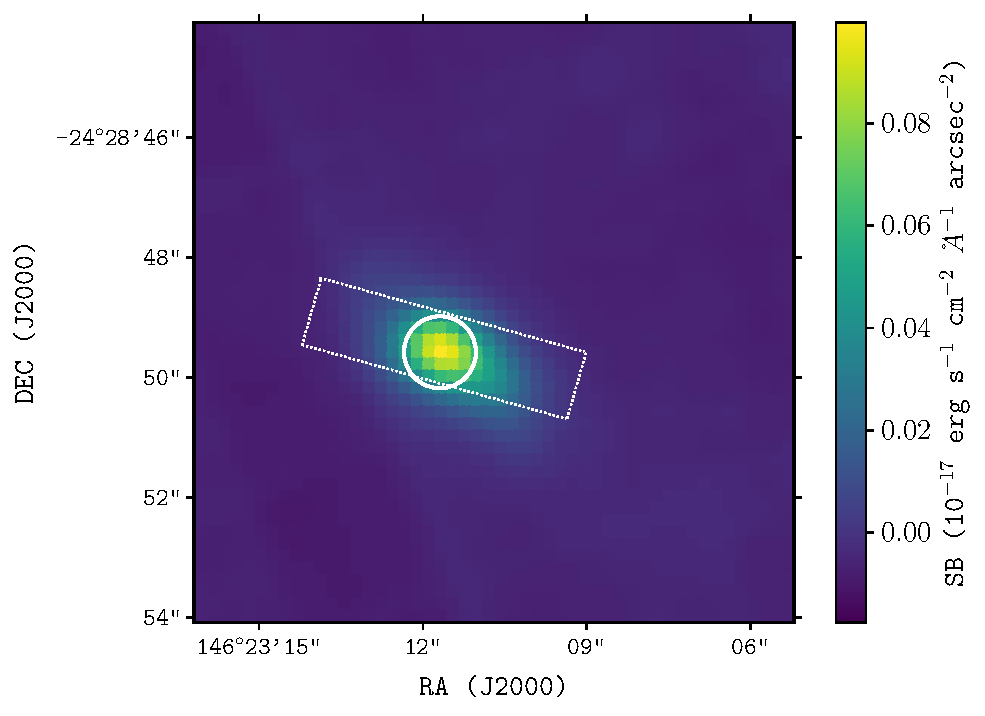
\includegraphics[width=0.7\columnwidth]{plots_chp3/0943-242_continuum_img.pdf}
\caption[MUSE line and continuum (white-light) image of MRC 0943-242]{MUSE line and continuum (white-light) image of MRC 0943-242. At the centre of the image is the high surface brightness region of the galaxy halo. The sub-cube aperture from which the spectrum in Fig. \ref{fig:0943-spectrum} is obtained is shown within the circle. The UVES slit (dotted outline) has a 1.2\arcsec width and extends over 5\arcsec.}
\label{fig:0943-continuum}
\end{figure}

\begin{sidewaysfigure*} 
\centering
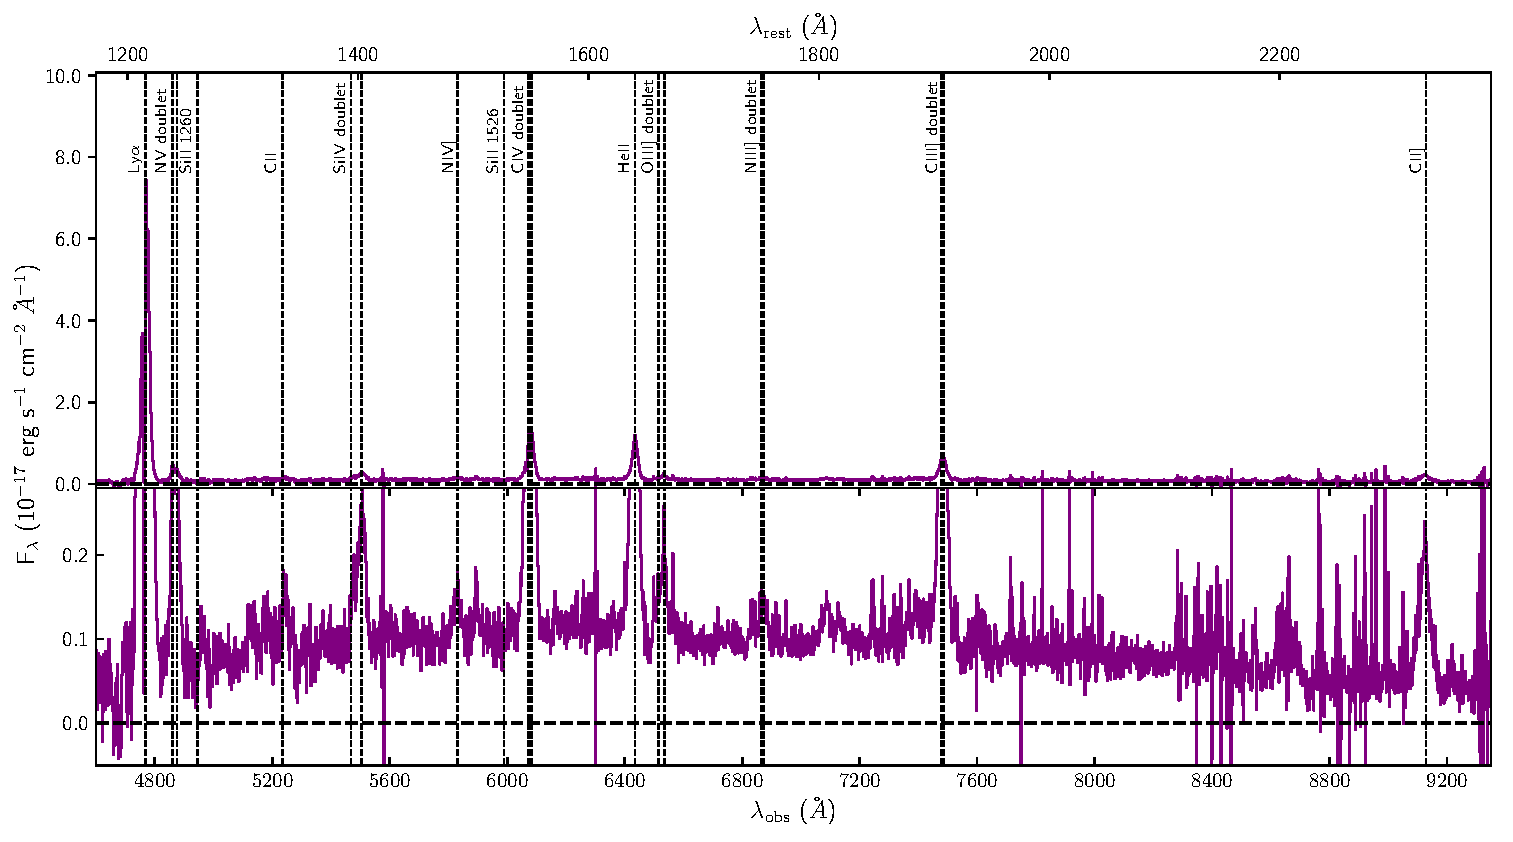
\includegraphics[width=\textwidth]{plots_chp3/0943-242_spectrum_3_pix_zoom.pdf}
\caption[MUSE spectrum of the bright nucleus in MRC 0943-243]{MUSE spectrum of the high surface brightness region in the halo of MRC 0943-243. The spectrum contains several rest-UV lines that are labelled and indicated by the dashed vertical lines. The upper panel shows the entire flux density range for the spectrum, while the lower panel covers only the low flux density range to show the lower S/N lines more clearly.}
\label{fig:0943-spectrum}
\end{sidewaysfigure*}

\subsection{Line-fitting procedure}
The goal of this work is to parametrise the physical conditions of gas in the halo of the radio galaxy Yggdrasil. To do this, we used the line profiles of ions that undergo resonant transitions, that is, \lya~$\lam$1216, \ion{C}{IV} $\lam\lam1548,1551$, \ion{N}{V} $\lam\lam1238,1243,$ and \ion{Si}{IV} $\lam\lam1393, 1402 $ (see Fig. \ref{fig:0943-spectrum}). We applied line-fitting procedures that combine Gaussian and Voigt models in order to characterise the emission and absorption simultaneously. The emergent emission is $F_\lam = F_{\lam,0} e^{-(\tau_{\lam,1} + ... + \tau_{\lam,n}) }$ for $n$ absorbers, where the unabsorbed emission, $F_{\lam,0},$ is denoted by the Gaussian function
\begin{equation}
F_{\lam,0} = \frac{ F }{ \sigma_\lam \sqrt{2\pi}} \exp\left[{-\frac{1}{2}\left(\frac{\lam - \lam_0}{\sigma_\lam}\right)^2}\right]
,\end{equation}
where $F$ is the integrated flux of the underlying emission, $\lam_0$ is the Gaussian line centre, $\sigma_\lam$ is the line width, and $\lambda$ is the wavelength.
The absorption is quantified by the optical depth, $\tau_\lam,$ which is denoted by the Voigt-Hjerting function
\begin{equation}
\tau_\lam = \frac{ N\sqrt{\pi} e^2 f \lam_0^2 }{ \Delta\lam_D m_e c^2 }H(a,u),
\end{equation}
where $N$ is the column density, $e$ (electron charge), $m_e$ (electron mass), and $c$ (light speed) are fundamental constants, and $f$ is the oscillator strength. $H(a,u)$ is the Hjerting function in which $a \equiv\frac{\Gamma\lam_0^2}{4\pi c \Delta\lam_D}$ and $u \equiv\frac{(\lam - \lam_0)}{\Delta\lam_D}$ such that $\Gamma$ is the Lorentzian width, $\Delta\lam_D$ is the Doppler parameter (also $b$ parameter), and $\lam - \lam_0,$ is the frequency shift from the line centre ($\lam_0$). $H(a,u)$ is obtained from the \citet{tepper-garcia2006} approximation, which is well suited for absorption systems that have column densities $ N/{\rm cm}^{-2} \leq10^{22}.$ When fitting the absorption, we also made the simplifying assumption that each cloud of absorbing gas covers the emission line region with a unity covering factor (C $\simeq$ 1.0).

We used the \pkg{python} package \pkg{lmfit} to carry out the non-linear least-squares fitting \citep{newville2016}. Our fitting method of choice was the Levenberg-Marquardt algorithm, which performs the $\chi^2$-minimisation that yields our best-fit results. In the figures, we report the reduced $\chi^2$-squared value, $\chi_\nu^2 = \chi^2/(N-N_i),$ where $N$ is the number of data points and $N_i$ is the number of free parameters. For each line, we calculated the local continuum level by masking the line emission and fitting a first-order polynomial to the surrounding continuum. The first-order polynomial was subtracted from both the line and continuum of \ion{He}{II} and Ly$\alpha,$ which are bright enough that not fitting the continuum has little effect on the overall fit. For \ion{C}{IV}, \ion{N}{V,} and \ion{Si}{IV}, which are lower in surface brightness (than \lya~and \ion{He}{II}), the continuum is likely to impact the overall fit.

Fitting Gaussian and Voigt functions simultaneously means that the composite model has many fit parameters. To prevent over-fitting and also to obtain a physical result, we used \lya~and \ion{He}{II} as initial guesses when we fitted underlying emission and absorption profiles to the \ion{C}{IV}, \ion{N}{V,} and \ion{Si}{IV}+\ion{O}{IV]} lines. 

From the \ion{He}{II} fit (described later in section \ref{section:Heii-fit}), we obtained the best-fit results for Gaussian fluxes (F$_\lam$), line widths ($\sigma_\lam$), and line centres ($\lam_0$). $\Delta\lam_{0,\ion{He}{II}}$ is the error on the fitted \ion{He}{II} line centre such that $\lam_{0,\ion{He}{II}} = 6436.09 \pm 0.30$ $\ang.$ The line centres are in agreement with the \ion{He}{II} systemic velocity (or zero velocity, which is fixed to the systemic redshift of the galaxy) within its uncertainties, that is, $\Delta\lam_{0,\ion{He}{II}} = 0.30$ $\ang$ = 10.3 km s$^{-1},$ under the assumption that all the emission originates from the centre of the halo. The \ion{He}{II} fit results for line width and the redshift of the line centre were set as initial guesses in Gaussian fits for emission in the resonant lines, \ion{C}{IV}, \ion{N}{V}, \ion{Si}{IV} and the non-resonant \ion{O}{IV],} which emits as part of the \ion{Si}{IV}+\ion{O}{IV]} intercombination line. Furthermore, we ensured that $F_\lam$ and $\sigma_\lam$ remain positive. 

To fit the \lya~absorption in the MUSE spectrum, we used the best-fit parameters from the literature \citep[i.e.][]{jarvis2003,wilman2004} as initial guesses in the fitting procedure. The best-fit \lya~absorber redshifts were passed on as initial guesses for absorber redshifts in the \ion{C}{IV}, \ion{N}{V,} and \ion{Si}{IV} line profiles. The initial guesses for column densities and Doppler parameters are based on rough estimates from the literature (i.e. \citealp{jarvis2003,wilman2004}, G16; S18). All three Voigt parameters have a limited parameter space over which a solution can be obtained. These parameter constraints are summarised in Table \ref{table:absorption-limits}. 

% redshift
In the fitting routine, some absorber redshifts were given more freedom to vary over a given parameter space than others because 
the ionisation energies of the different gas tracers, \ion{H}{I}, \ion{C}{IV}, \ion{N}{V,} and \ion{Si}{IV}, differ greatly such that E$_\ion{H}{I}$ = 13.6 eV, E$_\ion{C}{IV}$ = 64.5 eV, E$_\ion{N}{V}$ = 97.9 eV, and E$_\ion{Si}{IV}$ = 45.1 eV. It would be unrealistic to expect them to exist at exactly the same redshifts. 

% Doppler parameter
The minimum Doppler parameter permissible in the line-fitting is set by the lower limit of the MUSE spectral resolution, which suggests that an approximate lower limit of $b_{\rm min} \sim \sigma_\lam = 90$ km s$^{-1}$ / 2.3548 $\simeq$ 40 km s$^{-1}.$ We set a conservative upper limit of $b_{\rm max} = 400$ km s$^{-1}$ for \ion{C}{IV}, \ion{N}{V,} and \ion{Si}{IV} with the understanding that the absorbing gas is kinematically quiet in relation to perturbed gas regions that have FWHM $\geq$ 1000 km s$^{-1}.$ 

% column density
In general, \lya~absorbers in HzRG gas nebulae are found to have low column densities of $N_\ion{H}{I}/{\rm cm}^{-2} = 10^{13} - 10^{15}$ or be optically thick with column densities of $N_\ion{H}{I}/{\rm cm}^{-2} > 10^{18}$  \citep{wilman2004}. Because \ion{H}{I} is frequently more abundant than metals in halo gas environments, we can expect the column densities of the metal ions to be lower. Hence, we set the lower and upper limits for permissible fitted column densities to $N/{\rm cm}^{-2} = 10^{12} - 10^{20}$ cm$^{-2}.$ A full summary of the initial boundary conditions in the fitting procedure is given in Table \ref{table:absorption-limits}. The physical constraints placed on the line-fitting procedure by quantum rules are highlighted in Table \ref{table:absorption-rules}. 

\section{Best-fit line models}\label{section:best-fit-line}
\subsection{\ion{He}{II}}\label{section:Heii-fit}
\ion{He}{II} $\lam$1640 is the brightest non-resonant emission line and forms the basis of our estimation of the underlying emission profiles of the lines we study here, that is, Ly$\alpha,$ \ion{C}{IV}, \ion{N}{V,} and \ion{Si}{IV}. In the extracted spectrum, we obtained a detection of \ion{He}{II} emission that forms through cascade recombination of He$^{++},$ which emits a non-resonant photon. The \ion{He}{II} lines are often used to determine the systemic redshift of a galaxy (e.g. \citealp{reuland2007,swinbank2015}; S18). Although \lya~is brighter than \ion{He}{II}, we refrained from using \lya~for this purpose because of its susceptibility to radiative transfer effects that clearly affect the emergent line emission.

The \ion{He}{II} line, shown in Fig. \ref{fig:HeII-line}, has an excess of emission at $\Delta \varv \sim-1000$ km s$^{-1}$ that is not present at $\Delta \varv \sim1000$ km s$^{-1}$ , indicating asymmetry. This has been identified before in \citet{jarvis2003}, where the excess was found to have little effect on the final fit. Our 1D spectrum has brighter line detections, and to account for the excess emission in the wing, we therefore fit the \ion{He}{II} line with two Gaussian profiles: one for emission blueshifted relative to, and another for emission originating from, the systemic velocity. This method has been employed frequently for fitting asymmetric line profiles from various gas phases \citep[e.g.][]{mullaney2013,cicone2014,rakshit2018,hernandez-garcia2018,perna2019}. 

\begin{figure} 
\centering
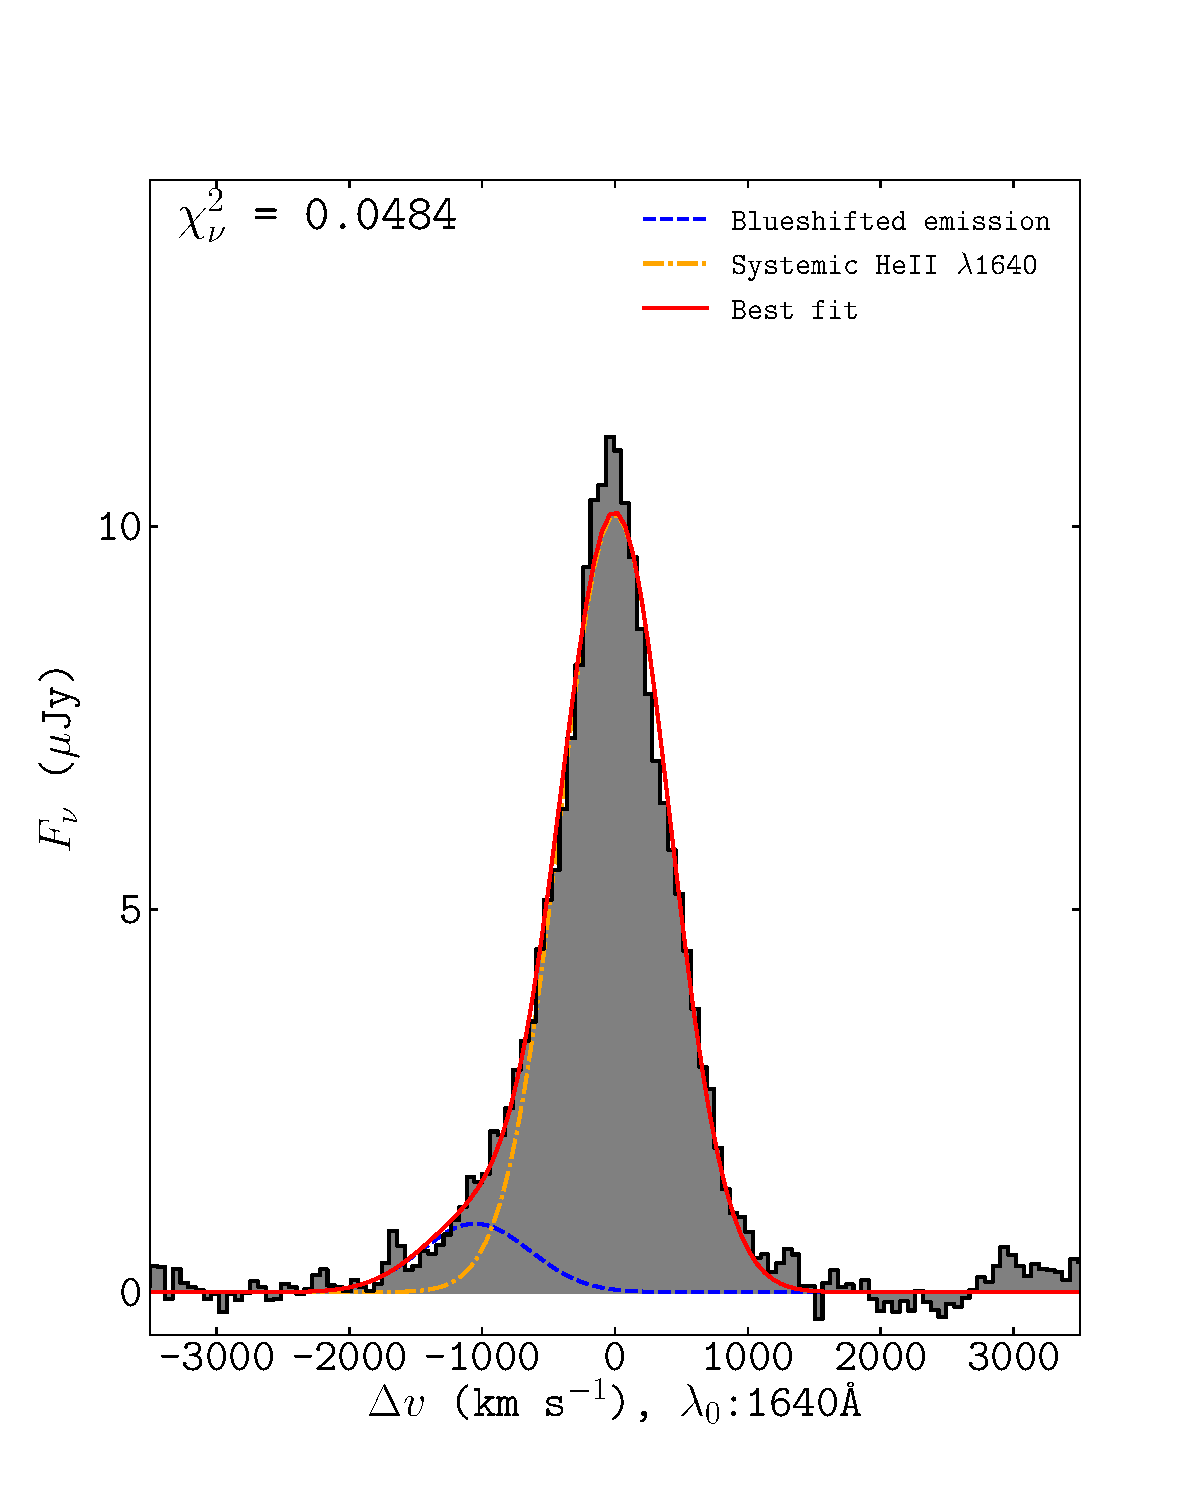
\includegraphics[width=0.6\columnwidth]{plots_chp3/HeII_fit.pdf}
\caption[\ion{He}{II} $\lam$1640 line in MUSE and its best-fit]{\ion{He}{II} $\lam$1640 line in the MUSE spectrum (shown in Fig. \ref{fig:0943-spectrum}). The line profile has been continuum subtracted. The best-fit model (red) consists of two Gaussian profiles. The first Gaussian component (in blue) models the excess blue wing emission at the negative velocities, while the second component (in orange) models the emission at the systemic velocity of the galaxy. }
\label{fig:HeII-line}
\end{figure}

We estimated the central velocity of the excess emission in \ion{He}{II} by spatially identifying where its emission peaks in surface brightness (explained further in section \ref{method:blueshifted-emission}). The best-fit Gaussian parameters obtained from the spatially offset region were used to fit the blueshifted emission as a second component to the emission from the HSBR at the systemic velocity. The result of this fitting procedure is shown in Fig. \ref{fig:HeII-line}, where the additional component is broadened to a line width of FWHM $\simeq1000$ km s$^{-1}$ and also blueshifted from the systemic velocity. From the \ion{He}{II} best-fit result, we obtain a fiducial systemic redshift of z$_{\rm sys}$ = $2.9235 \pm 0.0001$ that denotes the zero velocity for all the lines identified in Fig. \ref{fig:0943-spectrum}.

\subsection{\ion{H}{I} \lya}\label{section:Lya-fit}

\ion{H}{I} \lya~$\lam$1216 is the brightest line in the rest-UV spectrum. We fit the \lya~emission envelope with a double Gaussian: one to the non-absorbed singlet emission at the line centre, and another to the strong blue wing emission at $\Delta \varv \simeq -1000$ km s$^{-1}$ (see Fig. \ref{fig:Lya-line-muse-uves}). The motivation for including a second emission component to the \lya~fit is twofold: a) it is well detected in the emission line \ion{He}{II} and therefore likely to also emit in \lya, and b) there is an asymmetry between emission at the blue and red wings of Ly$\alpha.$ Once fit, we see that including a second Gaussian improved the \lya~emission fit. 

The updated Gaussian fit describes the \lya~profile well in both MUSE and UVES spectra and the best-fit parameters are in good agreement with the literature (see Tables \ref{table:absorption-fits-uves} and \ref{table:emission-fits-uves}). This is expected because \lya~is affected by radiative transfer effects and is therefore less likely to have a symmetric emission profile. There is also an additional underlying kinematic component causing the blue wing excess, based on the \ion{He}{II} line fit (see Fig. \ref{fig:HeII-line}). 

To account for the absorbers, we fit four Voigt profiles, as has been done in previous works on this topic (i.e. \citealp{vanojik1997,jarvis2003,wilman2004}; G16; B18). We also convolved the Voigt profiles with the line-spread function (LSF) of MUSE, using a fast-Fourier transform similar to that used to convolve Voigt and LSF profiles in the package, \pkg{vpfit} \citep{krogager2018}. The LSF or instrumental profile (IP) of MUSE, when convolved with the Voigt profile, has an average Gaussian width of $<\sigma_\lam>$ = 2.65 $\ang.$ 

We show the line-fitting result for \lya~in Fig. \ref{fig:Lya-line-muse-uves}a. Below this, in Fig. \ref{fig:Lya-line-muse-uves}b, we show a similar fit to the \lya~profile as was detected with UVES, which has an LSF with an average Gaussian width of $<\sigma_\lam>$ = 0.3 $\ang.$ 

\begin{figure} 
\centering
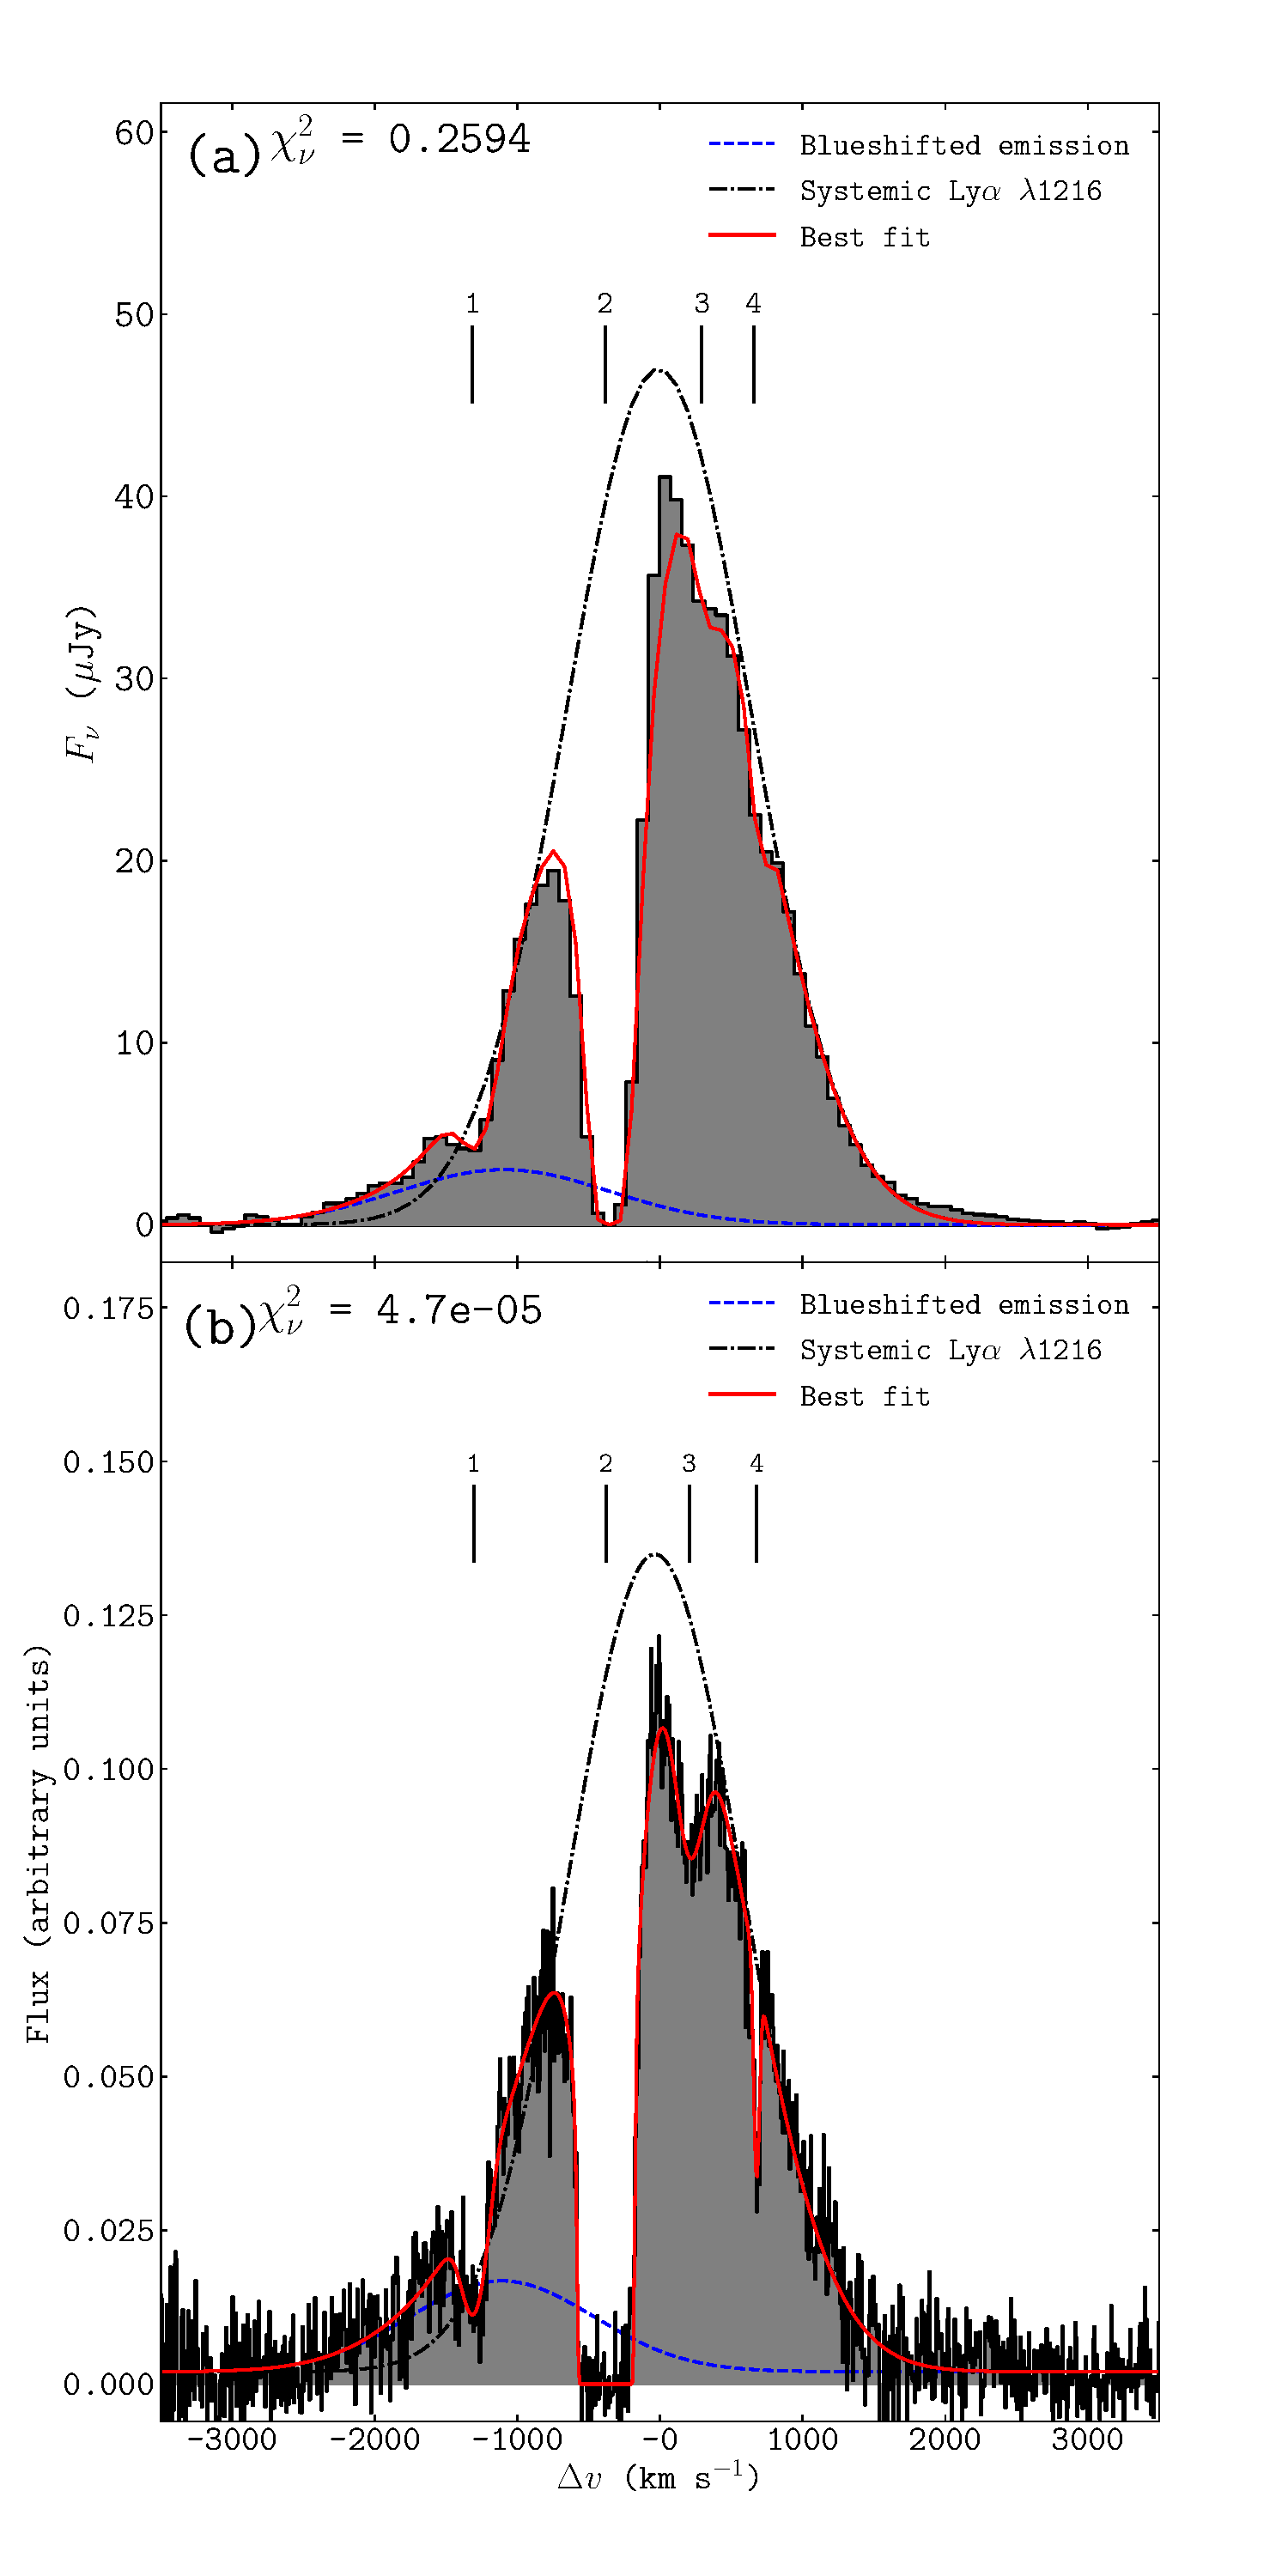
\includegraphics[width=0.6\columnwidth]{plots_chp3/Lya_fit_uves_muse_blue_fit.pdf}
\caption[\lya~$\lam1216$ line in MUSE and its best-fit]{MUSE-detected continuum-subtracted \lya~($upper$) and ancillary UVES-detected \lya~($lower$) for Yggdrasil. The best-fit line model (red) combines \lya~emission consisting of blueshifted and systemic components, as well as the four known absorption troughs.}
\label{fig:Lya-line-muse-uves}
\end{figure}

The \lya~absorber redshifts are used to predict the most probable redshifts for the absorbers, in general. In particular, the redshifts of the absorbers associated with resonant metal ions, \ion{C}{IV}, \ion{N}{V,} and \ion{Si}{IV}, are constrained to stay within $4\Delta{\rm z_{sys}}$  (where $\Delta{\rm z_{sys}} =1.35\e{-4}$) agreement of the measured \lya~absorber redshifts. This is done following the hypothesis that \lya~absorption occurs within roughly the same volume of gas as absorption of photons associated with the resonant transitions. 

For this to occur, there would need to be a very strong ionising continuum to produce all of the observed ions, which is possible with ionisation by the AGN. The different ionisation energies also imply that fixing the absorbers to exactly the same redshift is unrealistic. This is why we allowed the fitted absorber redshifts to vary over a parameter space that depends on how tightly a parameter needed to be constrained. 

\subsection{\ion{C}{IV} and \ion{N}{V}}\label{section:CIV-NV-fit}

We have obtained detections of \ion{C}{IV} $\lam\lam1548,1551$ and \ion{N}{V} $\lam\lam1238,1243$. Given that \lya~absorber 4 is narrow, it is likely to suffer the highest degree of instrumental broadening in MUSE, as seen in Fig. \ref{fig:Lya-line-muse-uves}b. For \ion{C}{IV} and \ion{N}{V}, we therefore did not include a fourth absorber in the model. At the MUSE spectral resolution we expect to lose any absorption signal from such a narrow absorber. The Voigt profiles were, as with Ly$\alpha,$  convolved with the LSF of MUSE. 

The observed emission in the doublet lines, \ion{C}{IV} and \ion{N}{V}, was fit with two Gaussian functions that were constrained according to atomic physics (all constraints are summarised in Table \ref{table:absorption-rules}). The local continuum was estimated using a  separate linear polynomial fit (to the continuum only, with line emission masked). The continuum was thus fixed during fitting. Additionally, in \ion{C}{IV}, we fit a second component to each of the doublet lines to account for the blueshifted emission seen in \ion{He}{II,} which has a similar S/N level as \ion{C}{IV}. \ion{N}{V} has a lower S/N than both of these lines, therefore the blueshifted emission is likely to be negligible in this fit. 

We obtained atomic constants such as rest wavelengths and oscillator strengths from the database provided by \citet{cashman2017}. For doublet lines, the ratios of line centres (i.e. $\lam_1/\lam_2$) and rest-frame wavelengths were fixed to one another. The doublet emission originates from the same gas, therefore the doublet line widths are equal, that is, $\sigma_{\lam,1} = \sigma_{\lam,2}$. The doublet ratios (DR = $F_1/F_2$) were fixed to the those of the oscillator strengths such that they are DR = 2. Doublet ratios of 2 are observed frequently in quasar absorption lines. This is particularly true for \ion{C}{IV} lines, whose doublet ratios vary from 2 to 1 from the linear to the saturated absorption regimes \citep{peroux2004}. Assuming that \ion{C}{IV} and \ion{N}{V} absorbers 1 and 3 are not saturated and have a unity covering factor, C $\simeq$ 1.0, because their emission does not reach zero flux level at the absorber velocities, we set DR = 2 when fitting.

The best-fit models for \ion{C}{IV} and \ion{N}{V} are shown in Figs~\ref{fig:CIV-and-NV-lines}a and \ref{fig:CIV-and-NV-lines}b. The emission and absorption fit results are shown in Tables \ref{table:absorption-fits} and \ref{table:emission-fits}, respectively. We note that both \ion{C}{IV} and \ion{N}{V} fits feature a slight kink at $\Delta \varv$ $\sim -2000$ km s$^{-1}.$ This may be the result of the column density of absorber 1 being over-estimated at this velocity, which could imply that the blueshifted \ion{C}{IV} emission is not impeded by absorber 1, as we have assumed. Rather, absorber 1 covers the emission line region behind it, the blueshifted emission. Determining which absorbers cover the systemic and/or the blueshifted emission is a task that will require higher spatial and/or spectral resolution. For simplicity, we assumed that all three absorbers impede the systemic, blueshifted, and continuum emission components.


\begin{figure}
        \subfloat[\ion{C}{IV} doublet line]{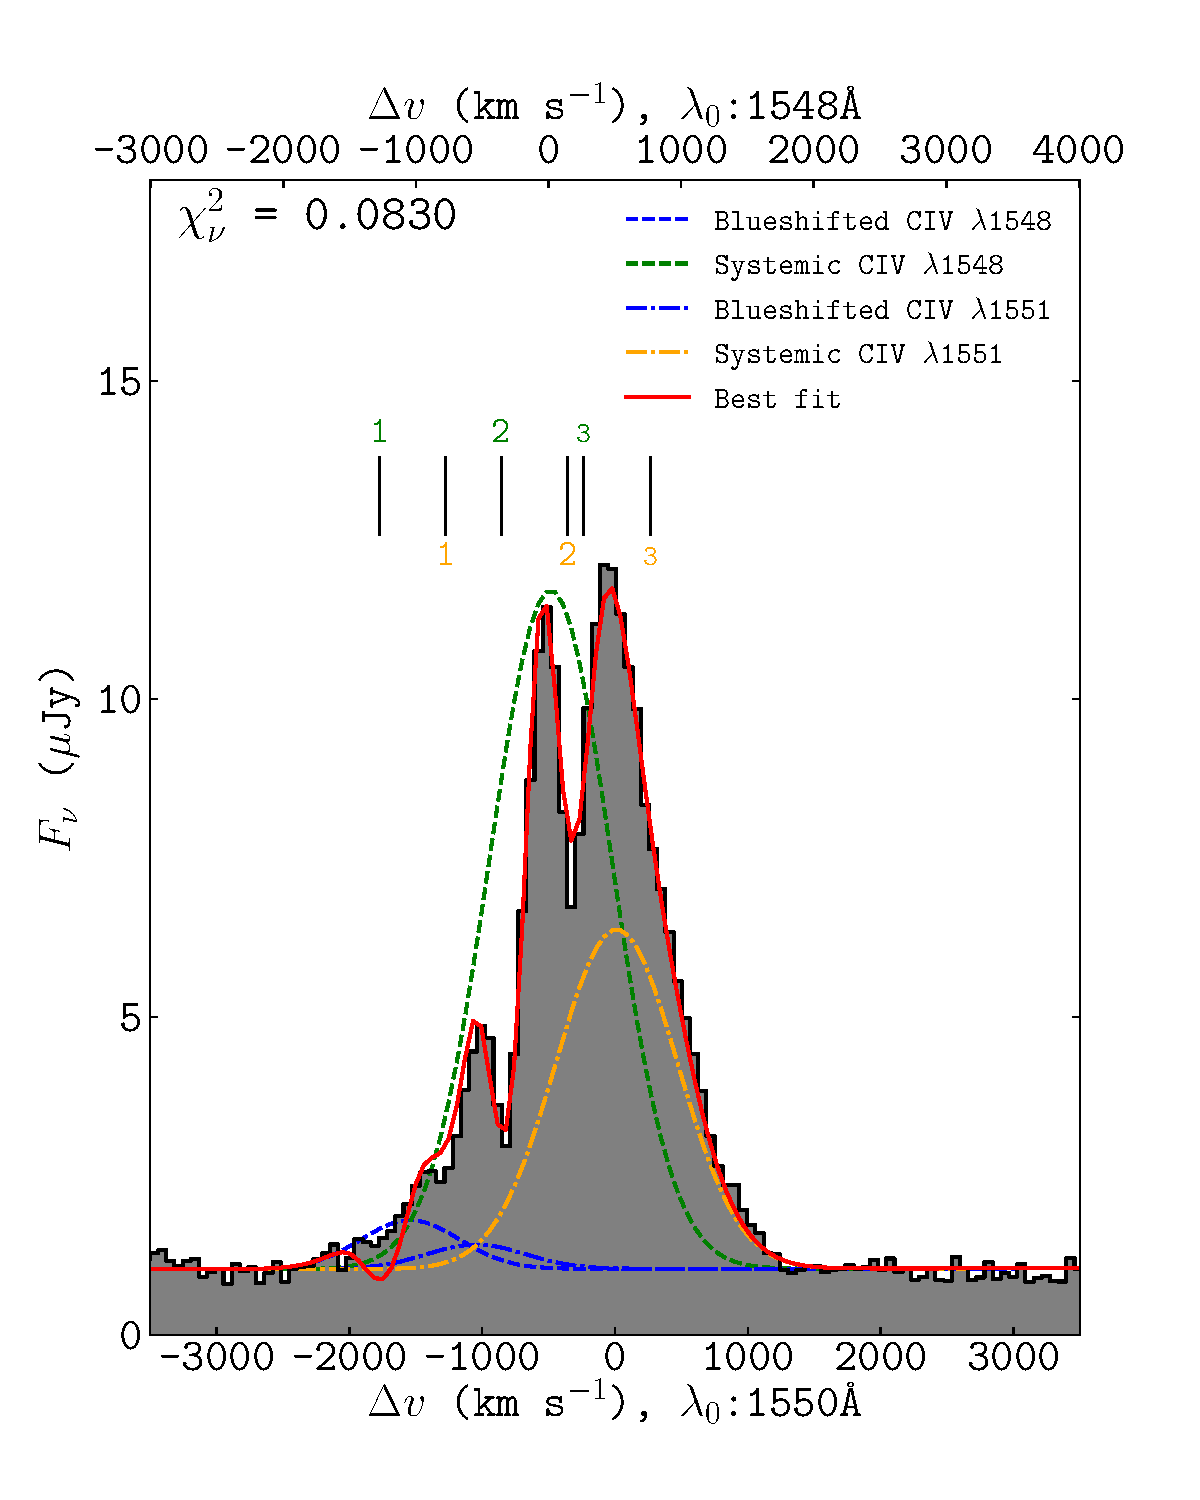
\includegraphics[width=0.52\columnwidth]{plots_chp3/CIV_fit.pdf}}
        \subfloat[\ion{N}{V} doublet line]{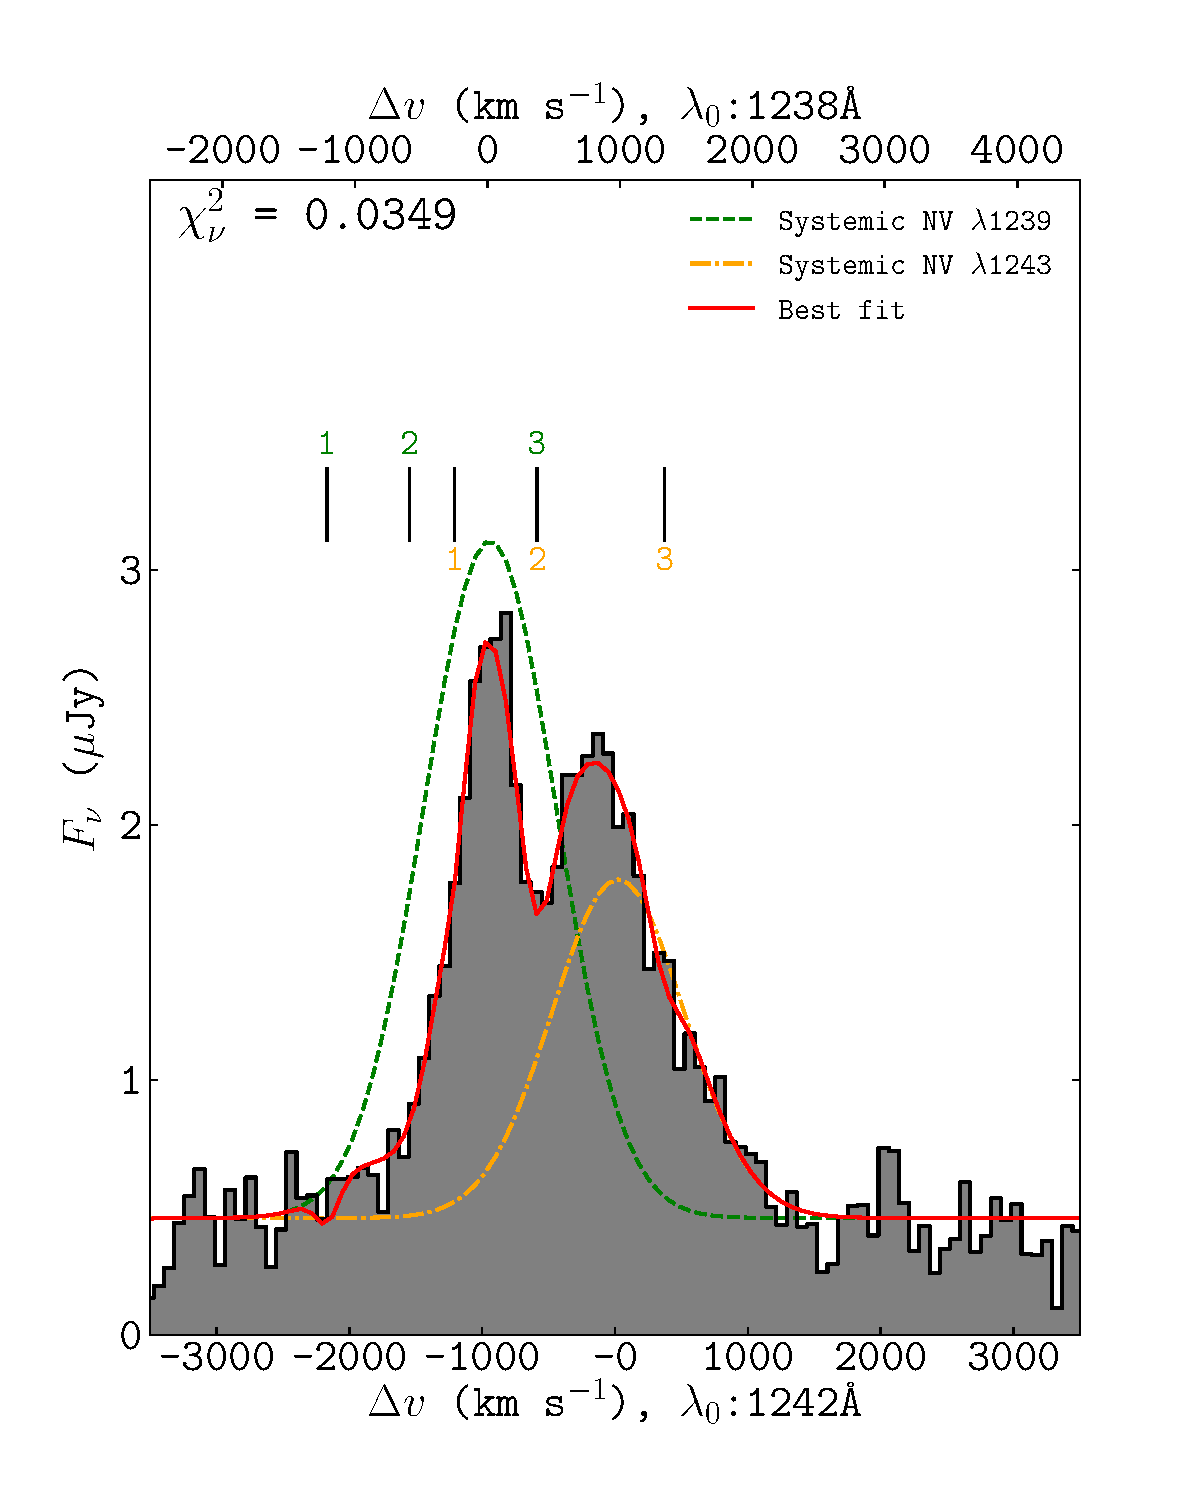
\includegraphics[width=0.52\columnwidth]{plots_chp3/NV_fit.pdf}}\\
\caption[\ion{C}{IV} $\lam\lam1548,1551$ and \ion{N}{V} $\lam\lam1238,1243$ lines in MUSE and their best-fits]{Panel (a): Best-fit line model fit to \ion{C}{IV} $\lam\lam1548,1551$ detected with MUSE. The green and orange dashed lines represent the underlying doublet emission at wavelengths of 1548 $\ang$ and 1551 $\ang,$ which are the rest-frame velocities, in the $\text{upper}$ and $\text{lower}$ axes, respectively. Three Voigt profiles model the absorbers for each emission line in the doublet. Panel (b): Best-fit line model for \ion{N}{V} $\lam\lam1238,1243$ detected with MUSE. The green and orange dashed lines represent the underlying doublet emission at wavelengths of 1548 $\ang$ and 1551 $\ang,$ which are the rest-frame velocities, in the $\text{upper}$ and $\text{lower}$ axes, respectively. Three Voigt profiles model the absorbers for each emission line in the doublet. }
\label{fig:CIV-and-NV-lines}
\end{figure}

% \begin{figure} 
% \centering
% 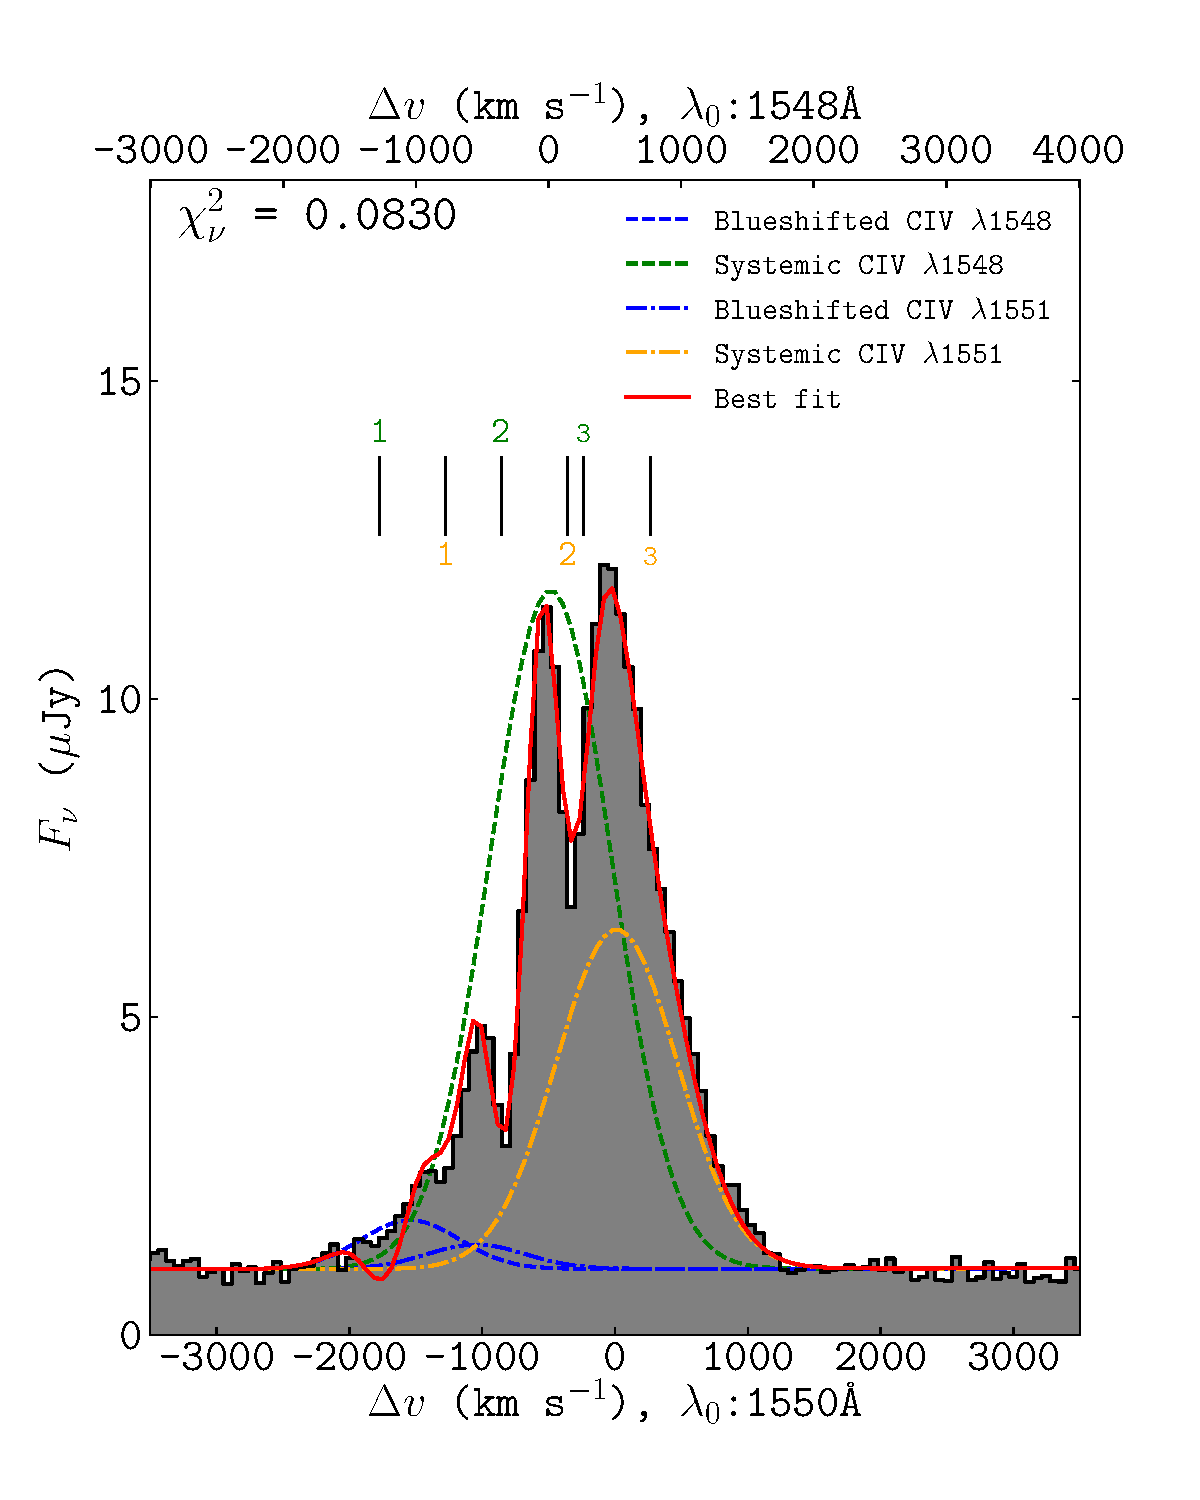
\includegraphics[width=0.6\columnwidth]{plots_chp3/CIV_fit.pdf}
% \caption{Best-fit line model fit to \ion{C}{IV} $\lam\lam1548,1551$ detected with MUSE. The green and orange dashed lines represent the underlying doublet emission at wavelengths of 1548 $\ang$ and 1551 $\ang,$ which are the rest-frame velocities, in the $\text{upper}$ and $\text{lower}$ axes, respectively. Three Voigt profiles model the absorbers for each emission line in the doublet.}
% \label{fig:CIV-line}
% \end{figure}

% \begin{figure} 
% \centering
% {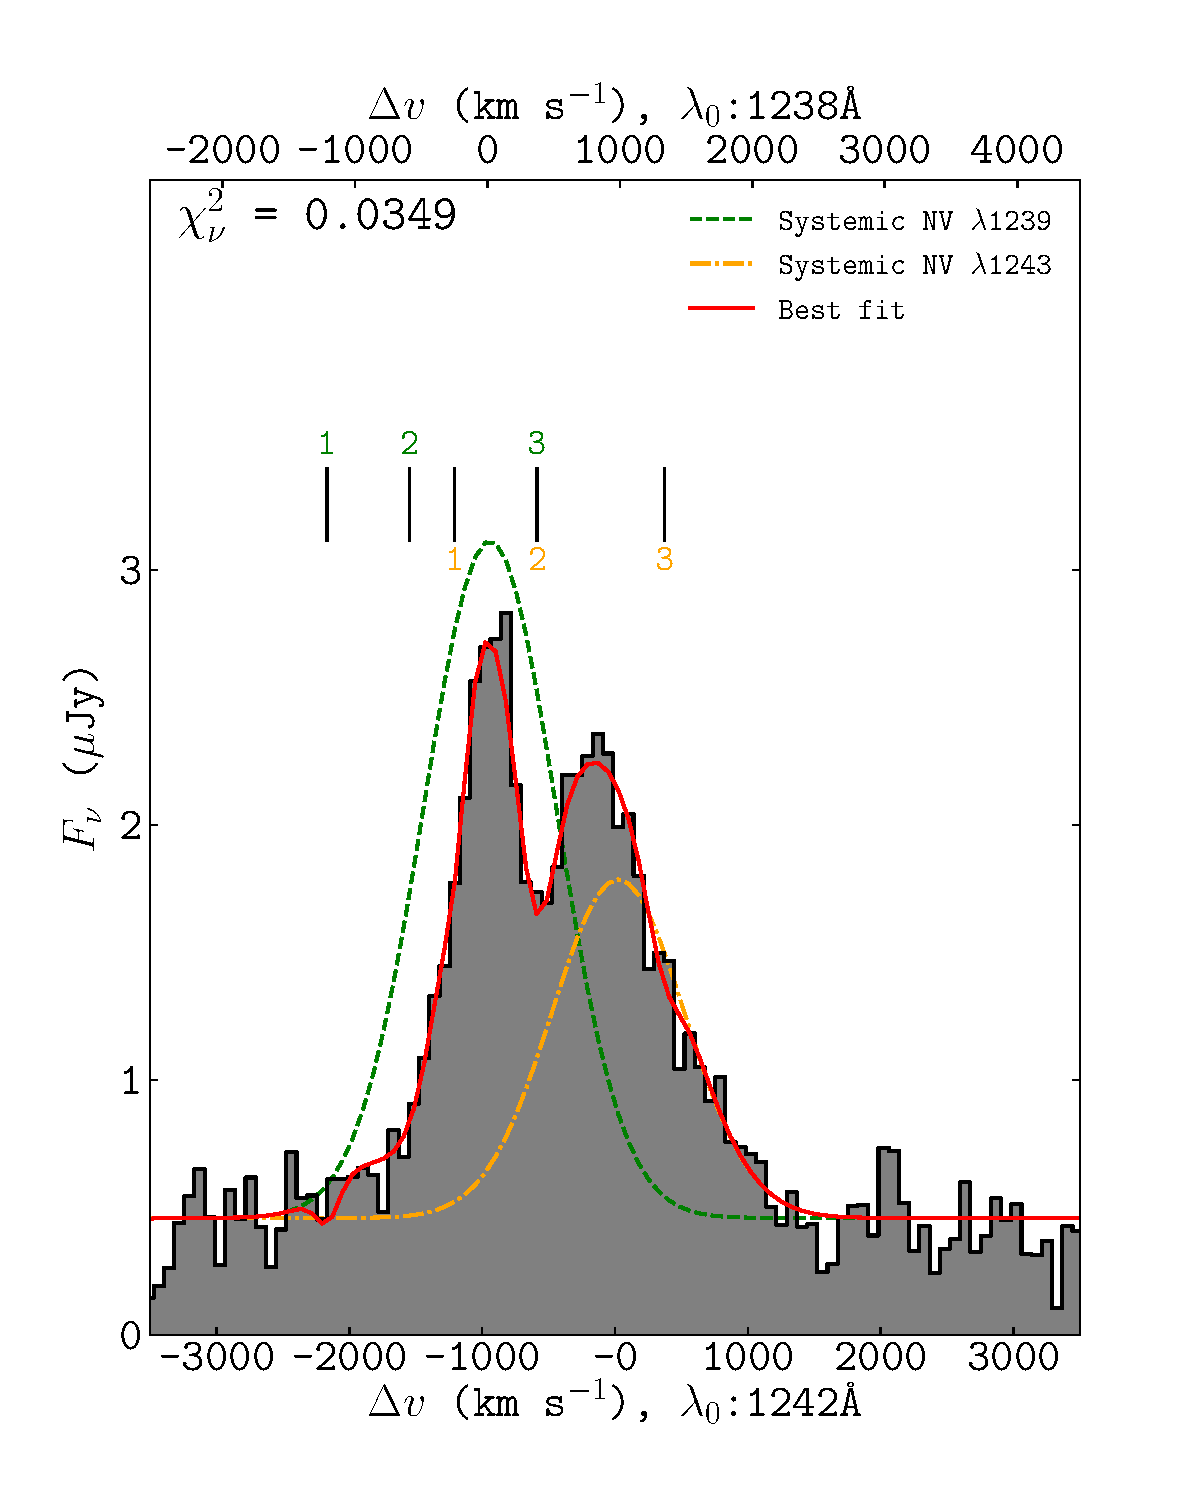
\includegraphics[width=0.6\columnwidth]{plots_chp3/NV_fit.pdf}}
% \caption{Best-fit line model to \ion{N}{V} $\lam\lam1238,1242$ detected with MUSE. The green and orange dashed lines represent the underlying doublet emission at the rest-frame wavelengths 1238 $\ang$ and 1242 $\ang,$ which are fixed to the systemic velocity in the $\text{upper}$ and $\text{lower}$ axes, respectively. Three Voigt profiles model the absorbers for each emission line in the doublet. }
% \label{fig:NV-line}
% \end{figure}

\begin{figure} 
\centering
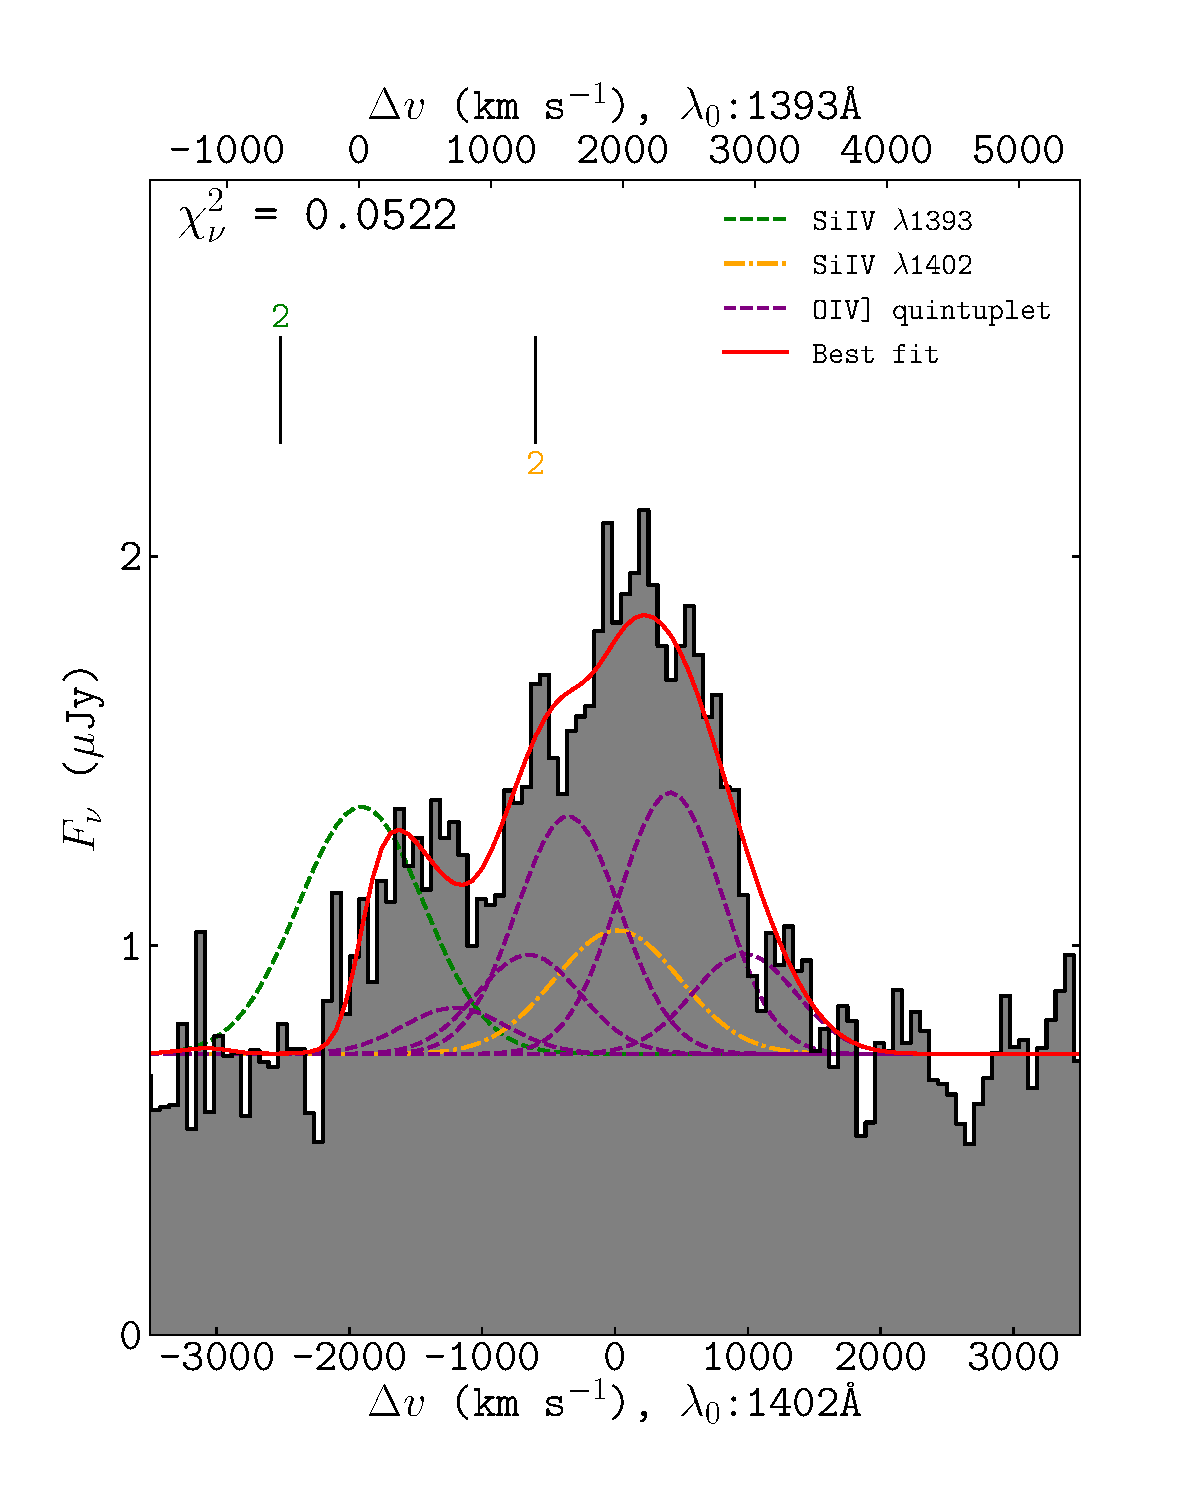
\includegraphics[width=0.55\columnwidth]{plots_chp3/SiIV_fit.pdf}
\caption[\ion{Si}{IV} $\lam\lam1393,1402$ + \ion{O}{IV]} intercombination line in MUSE and its best-fit]{Best fit line model to the intercombination \ion{Si}{IV} $\lam\lam1393,1402$ + \ion{O}{IV]} line detected with MUSE. The green and orange dashed lines represent the underlying doublet emission at the rest-frame wavelengths, 1393 $\ang$ and 1402 $\ang,$ which are fixed to the systemic velocity in the upper and lower axes, respectively. The \ion{O}{IV]} quintuplet line emission is shown in purple.}
\label{fig:SiIV-line}
\end{figure}

\subsection{\ion{Si}{IV}+\ion{O}{IV}]}\label{section:SiIV-fit}

The detected \ion{Si}{IV} $\lam\lam1393,1402$ line doublet overlaps with emission from the \ion{O}{IV]} quintuplet. \ion{Si}{IV} is a resonant line, and we modelled it with an absorption line at the same velocity as \lya~absorber 2. We did not include absorbers 1 and 3 because the fit did not change significantly when they were added.  

As before, the Voigt profile was convolved with the LSF of MUSE and the \ion{Si}{IV} doublet emission  was modelled by two Gaussians. Again, we fixed the continuum to the result of the linear polynomial fit of the local continuum (while the line emission was masked). The \ion{O}{IV]} quintuplet comprises five emission components at the rest-frame wavelengths for \ion{O}{IV],} which are 1397.2 $\ang$, 1399.8 $\ang$, 1401.2 $\ang$, 1404.8 $\ang$, and 1407.4 $\ang.$ To fit these, we used five Gaussian profiles with equal line widths. The quintuplet ratios were set by the oscillator strengths of each transition. We show the fit for the intercombination \ion{Si}{IV}+\ion{O}{IV]} lines in Fig.~\ref{fig:SiIV-line}, and the absorption fit results are shown in Table \ref{table:absorption-fits} and those for emission in Table \ref{table:emission-fits}. 

In an attempt to confirm the consistency of this result, we compared the fluxes of the same \ion{Si}{IV} and \ion{O}{IV]} lines detected at high spectral resolution for the binary symbiotic star RR Telescopii, which is shown in Fig. 5 of \citet{keenan2002}. The best-fit flux ratios for \ion{O}{IV]} are consistent with those of the high-resolution stellar spectrum, which is the perhaps the best observational comparison available for \ion{Si}{IV} and \ion{O}{IV]} intercombination line fluxes. 

\begin{table*}
\caption[Boundary conditions from line-fitting routine]{Lower and upper bounds placed on initial conditions in the line-fitting routine.
\newline {\it Note:}$\Delta$ is the largest permissible deviation (from the initial guess) imposed on a fit parameter.}
\centering
\begin{tabular}{ l  l }
\hline \hline
Fit parameters & Boundary conditions \\
                                                                                                                & \\
  \hline
                                                                                                                & \\
\bf{Gaussian (for emission):}                   & \\
                                                                                                                & \\
Line centre, $\lam_0$ (\ang)                                    & $\Delta \lam_0 = 0.3$ \\
Line flux, $F$ (erg s$^{-1}$ cm$^{-2}$) & $F \geq$ 0 \\
Line width, $\sigma_\lam$ (\ang)                        & $\sigma_\lam > 0$ \\                                                           
                                                                                                                & \\
 \hline
                                                                                                                & \\
\bf{Voigt (for absorption):}                            & \\
                                                                                                                & \\
\underline{Redshift, $z$:}                              & \\    
 \lya                                                                                                   &       $\Delta z_1 \leq 5.0\e{-3}$  \\
                                                                                                                &       $\Delta z_2 \leq 1.0\e{-3}$ \\
                                                                                                                &       $\Delta z_3 \leq 4.0\e{-3}$ \\
                                                                                                                &       $\Delta z_4 \leq 3.0\e{-3}$ \\
\ion{C}{IV}                                                                             & $\Delta z_n \leq 6.0\e{-4}$\\
\ion{Si}{IV} and \ion{N}{V}                             & $\Delta z_n \leq 6.0\e{-3}$\\
                                                                                                                                                & \\
\underline{Doppler parameter, $b$ (km s$^{-1}$):}                       & \\                                                                                                                              
Ly$\alpha,$ \ion{C}{IV}, \ion{N}{V,} and \ion{Si}{IV}                    & 40 $\leq b \leq$  400 \\
                                                                                                                                                & \\
\underline{Column density, $N$ (cm$^{-2}$): }   & \\
\lya                                                                                                                                    & 10$^{12}$ $\leq N \leq$ 10$^{20}$ \\
\ion{C}{IV}, \ion{N}{V,} and \ion{Si}{IV}                                & 10$^{13}$ $\leq N \leq$ 10$^{16}$ \\                    
                                                                                                                                                & \\
  \hline
\end{tabular}
\label{table:absorption-limits}
\end{table*}

\begin{table*}
\caption[Line constraints imposed by atomic physics]{Line constraints, set by atomic physics, are embedded in the fitting to obtain best-fit results for \ion{C}{IV}, \ion{N}{V,} and \ion{Si}{IV}+\ion{O}{IV]}. The flux ratios (${F_1}/{F_2}$) are equal to the oscillator strength ratios ($f_1/f_2$). The line centre ratios ($\lam_{0,1}/\lam_{0,2}$) are equal to the rest-frame wavelength ratios ($\lam_1/\lam_2).$ The redshift, $z,$ Doppler parameter, and column density, $N,$ are equal between doublet wavelengths. The \ion{O}{IV]} quintuplet constraints are similar to those of the doublets. The fourth quintuplet line, 1404.8 $\ang,$ is the brightest of the \ion{O}{IV]} quintuplets, therefore the other four \ion{O}{IV]} lines are fixed to it. }
\centering
\begin{tabular}{ l  l }
\hline \hline
Fit Parameters &  Rules \\
        & \\
 \hline
        & \\
 \underline{Gaussian parameters for doublet lines:}     & \\
        & \\
Line centre, $\lam_0$ (\ang)                                                    & $\frac{\lam_{0,1}}{\lam_{0,2}} = \frac{\lam_1}{\lam_2}$ \\
Line flux, $F$ (erg s$^{-1}$ cm$^{-2}$)         & $\frac{F_1}{F_2} = \frac{f_1}{f_2}$ \\
Line width, $\sigma_\lam$ (\ang)                                & $\sigma_{\lam,1} = \sigma_{\lam,2}$ \\
        & \\
  \underline{Gaussian parameters for the \ion{O}{IV]} quintuplet line ($n = 1, 2, 3, 5$):} & \\
        & \\
  Line centre,  $\lam_0$ (\ang)                                         & $\frac{\lam_{0,n}}{\lam_{0,4}} = \frac{\lam_n}{\lam_1}$ \\
  Line flux, $F$ (erg s$^{-1}$ cm$^{-2}$)       & $\frac{F_n}{F_4} = \frac{f_n}{f_4}$ \\
 Line width, $\sigma_\lam$ (\ang)                               & $\sigma_{\lam,4} = \sigma_{\lam,n}$ \\
        & \\
 \underline{Voigt parameters for multiplet lines with $n$ transitions:} & \\
        & \\
Redshift, $z$                                                                                   & $z_1 = z_n$ \\
Doppler parameter, $b$ (km s$^{-1}$)            & $b_1 = b_n$ \\
Column density, $N$ (cm$^{-2}$)                         & $N_1 = N_n$ \\
        & \\
\hline
\end{tabular}
\label{table:absorption-rules}
\end{table*}

\begin{table*}
\caption[\lya~$\lam1216$ absorption line best-fit results from MUSE and UVES 1D spectra]{Best-fit results to the absorbers in the UVES \lya~spectrum from this work and from \citet{jarvis2003} and \citet{wilman2004}.}
\centering
\begin{tabular}{c D{,}{\, \,\pm\, \,}{-3} D{,}{\, \,\pm\, \,}{-3} D{,}{\, \,\pm\, \,}{-3}   }
\hline\hline                    
Absorber                & \mc{Absorber redshift}                        & \mc{Column density}                                             & \mc{Doppler parameter}   \\
        \#                                      & z                                                                             & \mc{$N_{\ion{H}{I}}$ (cm$^{-2}$)}       & \mc{$b$ (km s$^{-1}$)}      \\ 
                                                                                                & & & \\
                                                \hline
                                                & & & \\
                                                UVES  & & & \\
                                                (this work) & & & \\
                1                               & 2.9063,0.0001         & (1.363,0.217) \e{14}  & 107,15\\
                2                               & 2.9185,0.0001         & (1.262,0.148) \e{19}  & 58,1 \\
                3                               & 2.9262,0.0001         & (5.166,0.824) \e{13}  & 133,15\\
                4                               & 2.9324,0.0001         & (2.232,0.310) \e{13}  & 25,4 \\
                                                & & & \\
                                                UVES  & & & \\
                                                (literature) & & & \\
                1                               &       2.9066,0.0062           & (1.047,0.314) \e{14}    & 88,45 \\
                2                               &       2.9185,0.0001           & (1.202,0.072) \e{19}    & 58,3 \\
                3                               &       2.9261,0.0005           & (3.548,0.568) \e{13}    & 109,35 \\
                4                               &       2.9324,0.0001           & (2.239,0.672) \e{13}    & 23,17 \\
                                                & & & \\
\hline
\end{tabular}
\label{table:absorption-fits-uves}
\end{table*}

\begin{table*}[ht]
\caption[\lya~$\lam1216$ emission line best-fit results from MUSE and UVES 1D spectra]{Best-fit results to the non-absorbed emission in the UVES spectrum. The flux units are arbitrary (arb.). Blueshifted lines are labelled by the abbreviation ``b.l.''.}    
\centering                          
\begin{tabular}{ l c D{,}{\, \,\pm\, \,}{-3} D{,}{\, \,\pm\, \,}{-3} D{,}{\, \,\pm\, \,}{-3} }
\hline\hline UVES  \\
\hline        
Line    &  
\mc{Line centre (rest)} & 
\mc{Line centre (obs.)} 
&\mc{Line flux}  
& \mc{Line width}   \\   
        &  
\mc{$\lam_0$ (\ang)} & 
\mc{$\lam$ (\ang)} & \mc{$F$ (arb. units)}
&\mc{FWHM (km s$^{-1}$)}  \\
&  &  \mc{} & \mc{} &\mc{}  \\ \hline     
&  &  \mc{} & \mc{} &\mc{}  \\
  \lya                                                  & 1215.67       & 4769.07,2.76    & 0.56,0.14     & 1427.67,82.47 \\    
  \lya~(b.l.)    & "                             & 4751.99,16.73         & 0.01,0.01       & 1525.40,779.05 \\            
                                                                &  &  \mc{} & \mc{} &\mc{} \\   
\hline                                   
\end{tabular} 
\label{table:emission-fits-uves}  
\end{table*}

\newpage
\begin{sidewaystable}
\caption[Best-fit absorption line results]{Best-fit results to the absorbers in the MUSE spectrum. The uncertainties reported are 1$\sigma$ error bars. The parameters that are prefixed by $\text{a tilde}$ are the parameters that were fit with either very large or null uncertainties in the least-squares fitting routine, implying that these values may be poorly constrained. The column density fit parameters with large uncertainties have been quoted as upper limits. Column (4) is the central wavelength of the absorber. Column (8) is the rest-frame equivalent width (E.W.) (for \ion{Si}{II} lines only). 
\newline {\it Note:} $^{a}$ \ion{Si}{II} $\lam1260$ and $^{b}$ \ion{Si}{II} $\lam1526$}
\centering                          
\begin{tabular}{l l D{,}{\, \,\pm\, \,}{-5} D{,}{\, \,\pm\, \,}{-3} D{,}{\, \,\pm\, \,}{-5} D{,}{\, \,\times\, \,}{-2} D{,}{\, \,\pm\, \,}{-5} D{,}{\geq \, \,}{3}}
\hline\hline    
MUSE \\
\hline          
Abs.    & 
Ion             & 
\mc{Redshift}   & 
\mc{Absorber wav.} &
\mc{Velocity}   & 
\mc{Column density}     & 
\mc{Doppler} & 
\mc{E.W.}  \\
\#      & 
 & 
\mc{$z$}                & 
\mc{$\lambda$ (\ang)} &
\mc{$\Delta \varv$ (km s$^{-1}$)}       & 
\mc{$N$ (cm$^{-2}$)}                                                            & 
\mc{$b$ (km s$^{-1}$)}  & 
\mc{W$_{\lam,0}$}    \\  
        &  &    &  \mc{} & \mc{} &\mc{} \\   \hline
        &  &    &  \mc{} & \mc{} &\mc{} \\
1       & \lya                          & 2.9063,0.0003         & 4748.74,0.51                  & -1315,672                       & (1.64 \pm 0.52),10^{14}               & 149,44  \\
        & \ion{N}{V}            & 2.9076,0.0008 & 4840.85,1.39          & -1212,1686              & \leq1.04,10^{14}                                      & \sim101 \\
        & \ion{C}{IV}   & 2.9068,0.0007 & 6048.40                               & -1278,1915              & \leq3.78,10^{14}                                      & 197,93 \\
        &                                       &                                                       &                                                               &  \mc{}                          & \mc{}                                                                         & \mc{} \\   
2       & \lya                          & 2.9184,0.0002         &       4763.54,0.28                 & -385,109                      & (1.63 \pm 0.46),10^{19}                 & 45,31          \\  
        & \ion{N}{V}            & 2.9158,0.0008         & 4851.01,1.26                  & -585,740                        & (9.40 \pm 4.10),10^{14}                       & 365,78  \\
        & \ion{Si}{IV}  & \sim2.9157            & 5457.49                               & \sim-598                        & \leq2.40,10^{15}                                      & \sim400  \\
        & \ion{C}{IV}   & 2.9188,0.0001         & 6067.05                               & -357,52                         & (4.52 \pm 1.29),10^{14}               & 162,22 \\
        & \ion{Si}{II}$^a$      & 2.9212,0.0001         & 4942.28,1.67          &  -175,293                       & \geq1.83\e{14}                                                &         & ,0.79 \\   
        & \ion{Si}{II}$^b$      & 2.9183,0.0006         & 5982.04,1.16          &  -397,461                       & \geq5.35\e{14}                                        &  & ,0.41 \\  
        &                                       &                                                       &                                                               &  \mc{}                          & \mc{}                                                                         & \mc{} \\   
3 & \lya                                & 2.9273,0.0009         & 4774.32,1.41                  & 293,412                         & (2.06 \pm 1.54),10^{13}               & \sim104 \\
        & \ion{N}{V}            & 2.9283,0.0006         & 4866.50                               & 370,363                         & \leq1.61,10^{14}                                      & 157,71\\
        & \ion{C}{IV}   & 2.9267,0.0006         & 6079.31                               & 248,297                         & \leq6.03,10^{13}                                      & 212,81 \\ 
        &                                       &                                                       &                                                               &  \mc{}                          & \mc{}                                                                         & \mc{} \\     
4 & \lya                                & 2.9321,0.0004 & 4780.14,0.67          & 658,442                         & (2.07 \pm 1.28),10^{13}               & \sim50 \\
        &                                       &                                                       &                                                               &  \mc{}                          & \mc{}                                                                         & \mc{} \\   
\hline
\end{tabular}
\label{table:absorption-fits}  
\end{sidewaystable}

\begin{table} 
\caption[Best-fit emission line results]{Best-fit results to non-absorbed emission in the MUSE spectrum. The uncertainties shown are 1$\sigma$ error bars. Values prefixed by $\text{a tilde}$ are results that were fit with very large or null uncertainties (as in Table \ref{table:absorption-fits}). Blueshifted lines are labelled by the abbreviation ``b.l.''.}    
\centering                          
\begin{tabular}{l c D{,}{\, \,\pm\, \,}{-3} D{,}{\, \,\pm\, \,}{-3} D{,}{\, \,\pm\, \,}{-3} }
\hline\hline                                                                         MUSE  \\
\hline            
Ion     &  
\mc{Line centre (rest)} & 
\mc{Line centre (obs.)} 
&\mc{Line flux}  
& \mc{Line width }   \\    
        &  
\mc{$\lam_0$ (\ang)} & 
\mc{$\lam$ (\ang)} 
&\mc{$F$ (10$^{-17}$ erg s$^{-1}$ cm$^{-2}$)}  
& \mc{FWHM (km s$^{-1}$)}   \\   
                &  &  \mc{} & \mc{} &\mc{} \\   
\hline 
                &  &  \mc{} & \mc{} &\mc{} \\   
   \lya         & 1215.67  	& 4769.50,2.65   & 158.5,63.8    & 1511,108  \\    
   \lya~(b.l.)  & "         & 4752.23,57.14  & \sim11.9      & \sim1302 \\  
   \ion{N}{V}   & 1238.82   & 4860.80,1.37   & 6.8,0.9       & 1180,87 \\
                & 1242.80   & 4876.49,1.37   & 3.4,0.5       & 1175,87\\ 
   \ion{Si}{IV} & 1393.76   & \sim5468.70    & \sim1.4       & \sim1118  \\
                & 1402.77   & \sim5504.05    & \sim0.7       & \sim1111 \\
   \ion{O}{IV]} & 1397.20   & \sim5481.60    & \sim0.2       & \sim920 \\
                & 1399.80   & \sim5491.80    & \sim0.5       & \sim918 \\
                & 1401.20   & \sim5497.29    & \sim1.1       & \sim917 \\
                & 1404.80   & \sim5511.42    & \sim1.2       & \sim915 \\
                & 1407.40   & \sim5521.62    & \sim0.5       & \sim913 \\
   \ion{C}{IV}  & 1548.20   & 6074.59,1.78   & 20.4,3.1      & 1090,99   \\ 
   \ion{C}{IV} (b.l.) & "   & 6053.16,20.43  & \leq1.2  	 & \sim877 \\
   \ion{C}{IV} 	& 1550.77   & 6084.68,1.78   & 10.2,1.5      & 1088,99  \\
   \ion{C}{IV} (b.l.) & "   & 6063.21,20.39  & \leq0.6       & \sim756 \\                                                                      
   \ion{He}{II} & 1640.40   & 6436.09,0.30   & 16.4,0.5      & 978,24   \\ 
   \ion{He}{II} (b.l.) & "  & 6413.49,3.05   & 1.4,0.5       & 970,225  \\           
   \ion{C}{iii]} & 1906.7   & \sim7481.21    & \sim7.4       & \sim977 \\
   \ion{C}{iii]} (b.l.) & " & \sim7454.92    & \leq0.5       & \sim947 \\
   \ion{C}{iii]} & 1908.7   & \sim7489.06    & \sim3.7       & \sim976 \\
   \ion{C}{iii]} (b.l.) & " & \sim7462.74    & \leq0.2       & \sim946 \\
   \ion{C}{ii]} & 2326.9    & \sim9129.26    & \sim4.0       & \sim1300 \\
   \ion{C}{ii]} (b.l.) & "  & \sim9096.15    & \sim1.2       & \sim1152 \\             
       			&  &  \mc{} & \mc{} &\mc{} \\   
\hline                                   
\end{tabular} 
\label{table:emission-fits}  
\end{table}

\subsection{\ion{Si}{II}}\label{section:SiII-fit}

We have detected \ion{Si}{II} $\lam$1260 and \ion{Si}{II} $\lam$1527 absorption in the rest-UV spectrum. They were fit with Gaussians to account for the absorbed components (see Figs. \ref{fig:SiII_1260-fit} and \ref{fig:SiII_1526-fit}). Using this fit, we estimated their velocity shifts and column densities using the approximation from \citet{humphrey2008b}, 
\begin{equation}
N \geq \frac { W_\lam m_e c^2 } { \pi e^2 f \lam_0^2 },
\end{equation}
where $N$ is the column density, W$_\lam$ is the observed equivalent width, $m_e$ is the electron mass, $c$ is the light speed, $e$ is the electron charge, $f$ the oscillator strength, and $\lam_0$ the rest wavelength of the line. The column densities are lower limits because it is not possible to determine whether the lines are in the linear or logarithmic (flat) part of the curve of growth.

The column densities of the \ion{Si}{II} lines place them in the category of weak absorbers. Their velocity shifts are in agreement with that of \lya~absorber 2, meaning that these absorptions also occur within roughly the same gas volume as those of \ion{H}{I}, \ion{C}{IV}, \ion{N}{V}, and \ion{Si}{IV} absorbers (as Fig. \ref{fig:abs-vel} shows). This implies that the high column density  absorber is more probably matter bounded\footnote{A matter-bounded cloud is insufficiently optically thick to absorb all of the incident UV photons.}. For absorber 2 to be matter bounded, low-ionisation species such as \ion{Si}{II} would exist only in trace amounts compared to higher ionisation lines. A clear detection of both these ions at the same velocity as the strong absorber proves that the absorber is more probably ionisation bounded and has a unity covering factor. This also implies that ionising photons will not be able to escape from the CGM of this source and that ionising radiation emerging from the halo will not contribute significantly to the metagalactic background or ionisation of gas in the IGM.

\begin{figure}
\centering 
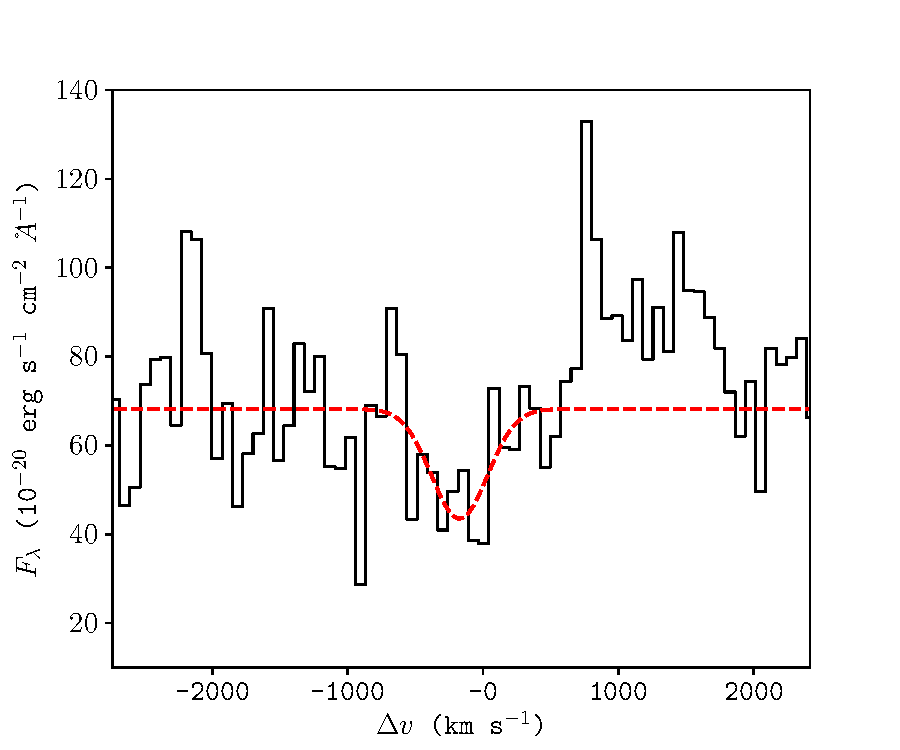
\includegraphics[width=0.75\textwidth]{plots_chp3/SiII_1260.pdf}
\caption[\ion{Si}{II} $\lam$1260 absorption line in MUSE and its best fit]{\ion{Si}{II} $\lam$1260 absorption line fit by a single Gaussian component (shown in red). }
\label{fig:SiII_1260-fit}
\end{figure}

\begin{figure}
\centering 
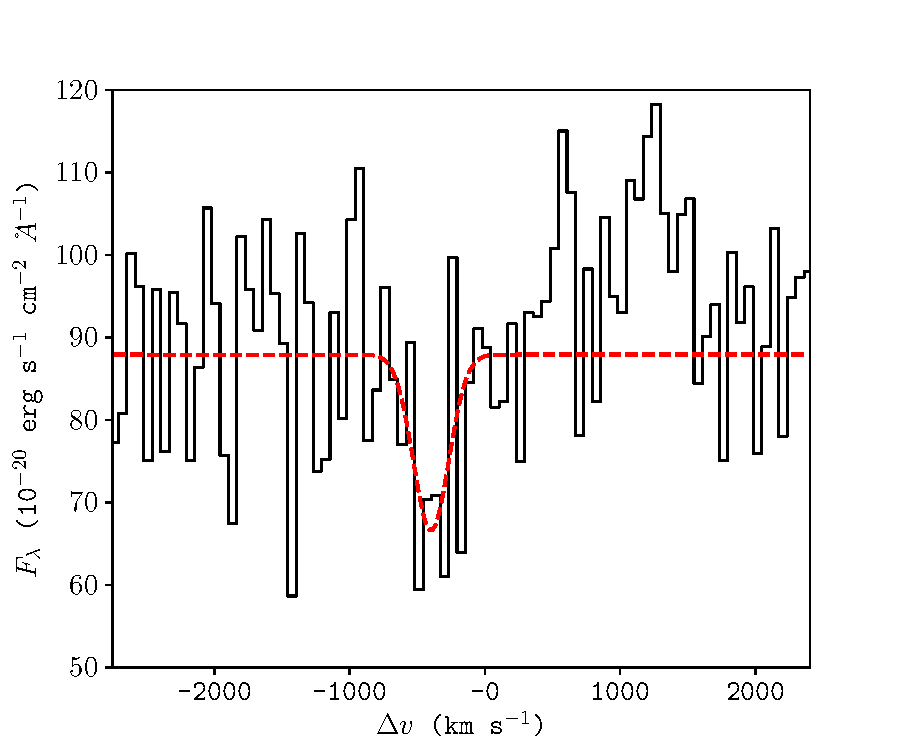
\includegraphics[width=0.75\textwidth]{plots_chp3/SiII_1526.pdf}
\caption[\ion{Si}{II} $\lam$1527 absorption line in MUSE and its best fit]{\ion{Si}{II} $\lam$1527 absorption line fit by a single Gaussian component (shown in red). }
\label{fig:SiII_1526-fit}
\end{figure}

\begin{figure*} 
\centering
 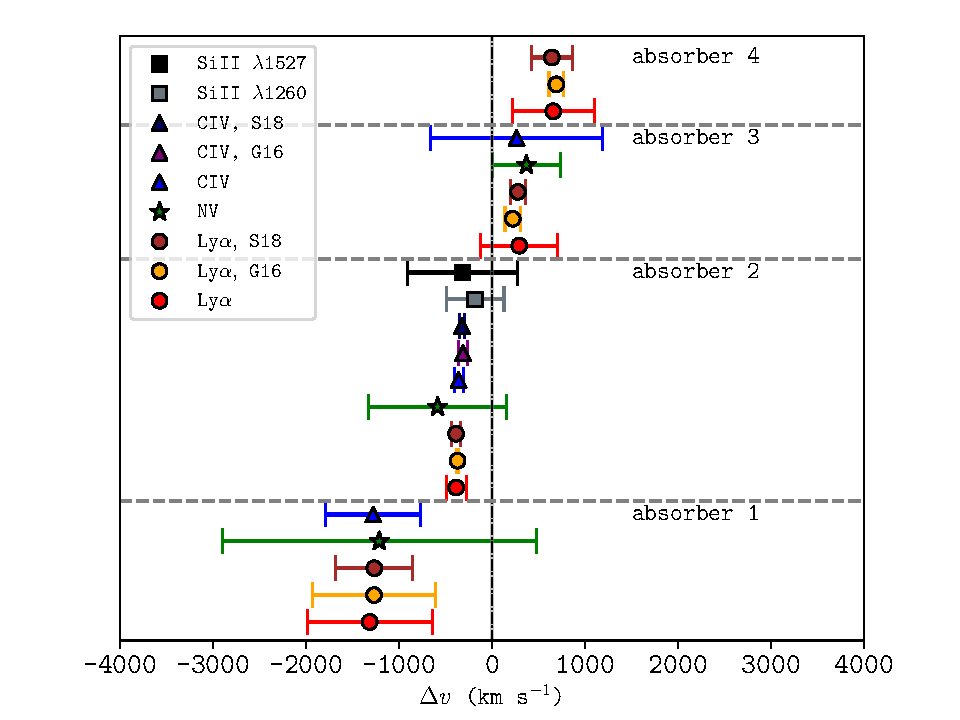
\includegraphics[width=0.75\textwidth]{plots_chp3/absorber_velocities.pdf}
 \caption[Velocity shifts of absorbers for resonant ions]{Relative velocities of Ly$\alpha,$ \ion{N}{V,} and \ion{C}{IV} and \ion{Si}{II} absorbers from this work as well as those from G16 and S18. The vertical dash-dotted (black) line indicates the systemic velocity and its error shown by the narrow shaded grey region. The horizontal dashed lines (grey) distinguish between the different absorbers.}
 \label{fig:abs-vel}
\end{figure*}

\subsection{\ion{C}{III]} and \ion{C}{ii]}}
The gas tracers \ion{C}{III]} $\lam\lam1906,1908$ and \ion{C}{II]} $\lam2326$ are non-resonant lines but useful tracers when searching for evidence of shock ionisation, which we discuss in more detail in section \ref{section:photoionisation-modelling}. We therefore included them in the line-fitting routine. To the \ion{C}{III]} doublet, we fit four Gaussian components in total to account for emission from the doublet at both systemic and blueshifted velocities as we have done for Ly$\alpha,$ \ion{He}{II,} and \ion{C}{IV}. \ion{C}{III]} has a sufficiently high surface brightness for us to fit it in the same way. Its best-fit result is shown in Fig. \ref{fig:CIII]-and-CII-fit}a. \ion{C}{II]} is a singlet that showed evidence of very blueshifted emission relative to systemic, and thus we also added an additional Gaussian component when fitting it (see Fig. \ref{fig:CIII]-and-CII-fit}b). The best-fit emission parameters for both of these lines are shown in Table \ref{table:emission-fits}.

\begin{figure} 
\centering
 \subfloat[]{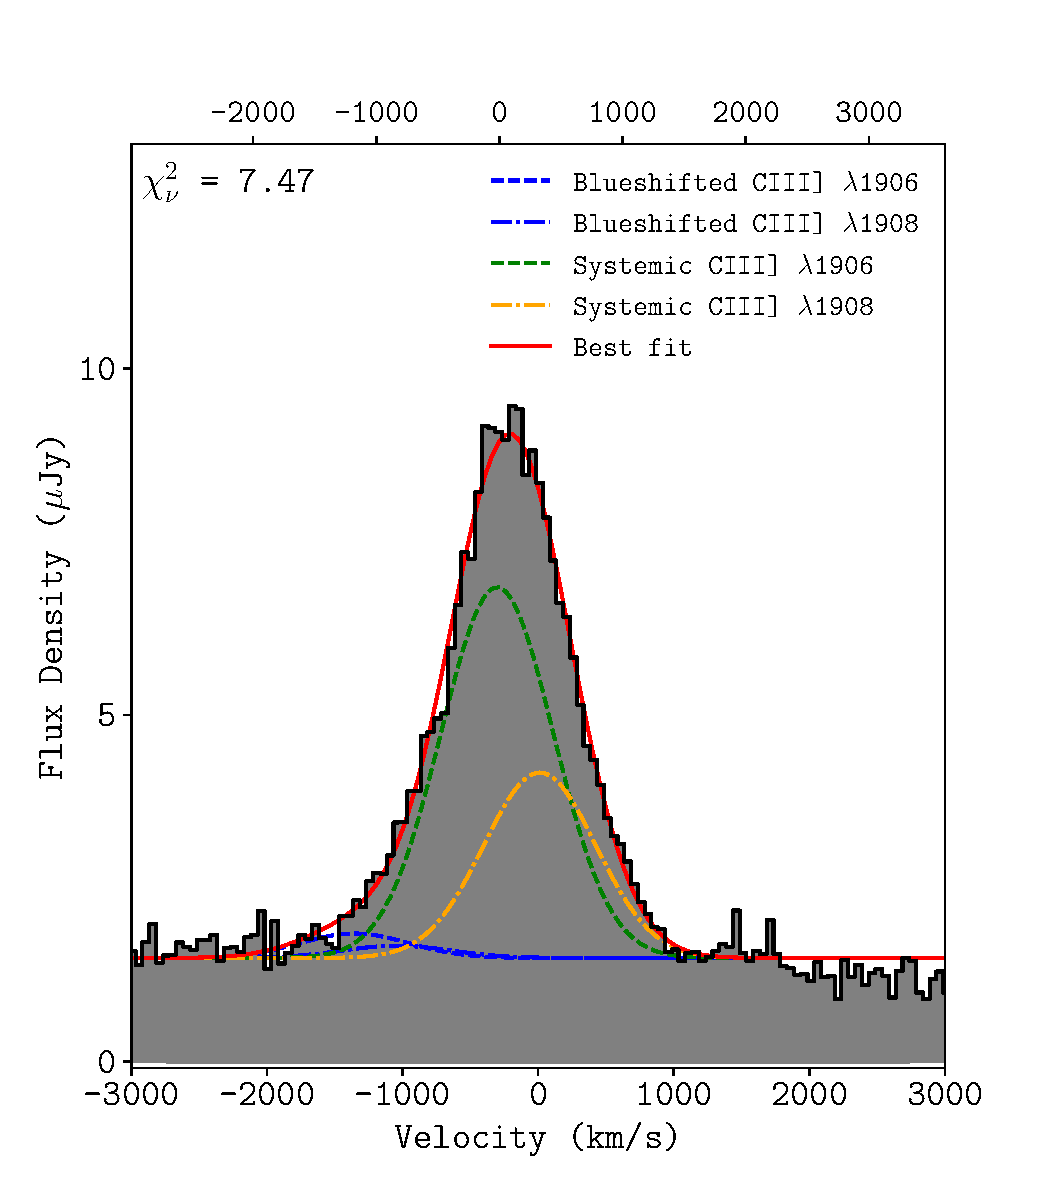
\includegraphics[width=0.5\textwidth]{plots_chp3/CIII]_fit.pdf}}
 \subfloat[]{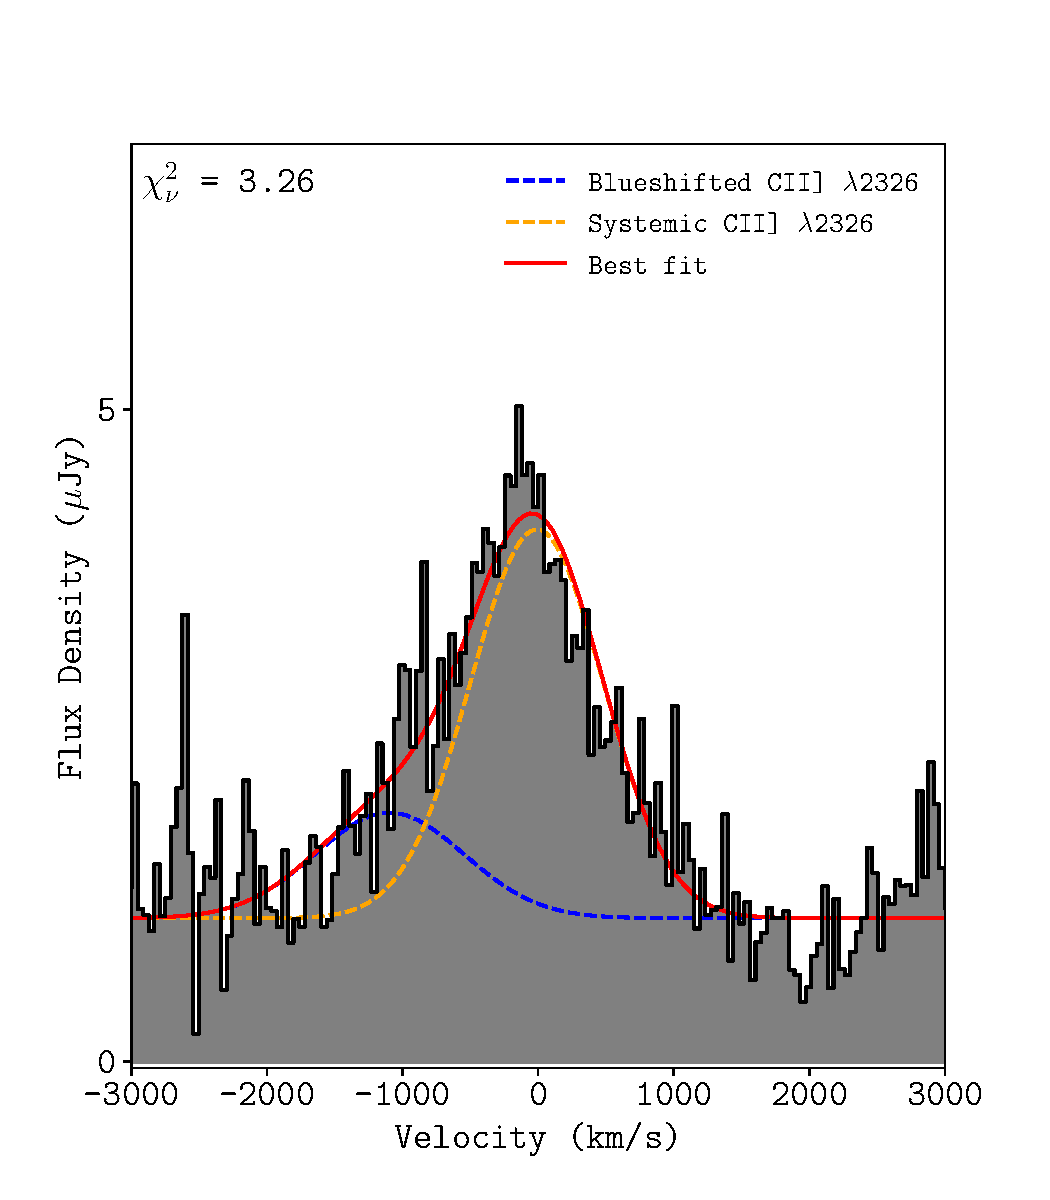
\includegraphics[width=0.5\textwidth]{plots_chp3/CII]_fit.pdf}}\\
 \caption[\ion{C}{III]} $\lam1906,1908$ and \ion{C}{II} $\lam 2326$ lines and their best-fits]{Panel (a): The \ion{C}{III]} $\lam1906,1908$ doublet line fit. Panel (b): The \ion{C}{II} $\lam 2326$ singlet line fit. Evidence for a blueshifted emission component is visible in both lines.}
\label{fig:CIII]-and-CII-fit}
\end{figure}


\section{Morphology of the absorbers}\label{section:morphology-absorbers}
The morphology of the absorbers within the circumgalactic medium of Yggdrasil is a focus of interest because much uncertainty about their origin and probable fate still remains, although the absorbers have been studied extensively using data from long-slit \citep[i.e.][]{rottgering1995,vanojik1997} and echelle spectroscopy \citep[i.e.][]{jarvis2003,wilman2004}, which were limited in their ability to provide a spatially resolved view of the gas in emission and absorption around Yggdrasil. In particular, they were not capable of showing the spatial variation in the \lya~profile that indicates variation in the kinematics of the most extended absorber (absorber 2). 

The MUSE data we used to perform resonant line-fitting above provide us with the capability of estimating the full extent and shape of \lya~absorber 2, which has a covering factor of C $\simeq$ 1.0, as G16 and S18 have shown. Furthermore, we can deduce its neutral and also ionised gas mass, and thus estimate its total hydrogen gas mass. 

\subsection{Size, shape, mass, and ionisation of the strongest \lya~absorber}\label{section:morphology}

In agreement with previous work on the \lya~line in Yggdrasil, absorber 2, located at a velocity shift of $\Delta \varv \sim-400$ km s$^{-1},$ reaches zero flux at its line centre. This implies that it is saturated with a unity covering factor, that is, C $\simeq$ 1.0 and \lya~column density of $\sim$ $10^{19}$ cm$^{-2}$ (see Table \ref{table:absorption-fits}). In the UVES spectrum, the \lya~absorbers occupy disparate velocities. This implies that the structure of the \ion{H}{I} gas is likely to be shell-like, as \citet{binette2000} and \citet{jarvis2003} have suggested. Guided by these previous findings and using more recent IFU data, we can estimate the size, shape, and mass of absorber 2, which is the strongest \lya~absorber. 

In terms of location, we relied on the result given in \citet{binette2000}, who showed that the absorbing and emitting gas are not co-spatial. Rather, absorber 2 is farther out of the halo and screens the radiation from the extended emission line region. We base the rest of our description of the halo gas on this predication. The spatial extent of the absorbing \ion{H}{I} gas medium in \citet{rottgering1995} is found to be $r \gtrsim 13$ kpc based on the extent of the measured \lya~emission and on the assumption of a unity covering factor for the associated absorption. In G16, visual inspection of the IFU data led to a value of $r \gtrsim 60$ kpc in radial extent. In S18, a velocity gradient across the halo was measured and used to estimate the absorber size, which the authors found to be $r \gtrsim 38$ kpc in radius. Here, we used the radial size of the \ion{H}{I} gas shell from G16, who determined the size by pinpointing the farthest spaxels from the nucleus of the gas halo at several position angles where the \lya~absorber 2 is still observed. 

In our data, we find that the absorber extends to projected distances of between $r = 50$ kpc and $r = 60$ kpc from the HSBR and is non-isotropic, covering the EELR over an area of 50 $\times$ 60 kpc$^{2}.$ A low surface brightness halo with quiescent kinematics (FWHM = 400 - 600 km s$^{-1}$) extending out to $r = 67$ kpc has been detected in this source \citep[e.g.][]{villar-martin2003}. Ly$\alpha,$ \ion{He}{II}, \ion{N}{V,} and \ion{C}{IV} emission are detected in the giant halo. In fact, \ion{N}{V} appears to be strengthened more than in the quiescent haloes of other HzRGs in \citet{villar-martin2003}. Given the size of the absorber, it is likely that it covers the emission from the giant halo. 

Assuming spherical symmetry and density homogeneity of the absorbing gas shell, the \ion{H}{I} mass is estimated to be $M_\ion{H}{I} = 4 \pi r^2 {\rm m}_\ion{H}{I} N_\ion{H}{I}$ \citep{deBreuck2003,humphrey2008b}. When we take into account the estimated size of $r \gtrsim 60$ kpc and an \ion{H}{I} column density of $10^{19.2}$ cm$^{-2}$ (from Table \ref{table:absorption-fits}), the \ion{H}{I} mass of absorber 2 is $M_\ion{H}{I}/\rm{M}_\odot = 5.7\e{9} (r / 60 {\rm kpc})^2$ $(N_\ion{H}{I} / 10^{19.2} {\rm cm}^{-2}).$ Our results agree to within at most two orders of magnitude with those in the literature. \citet{rottgering1995} estimated the mass of absorber 2  as $ M_\ion{H}{I}/\rm{M}_\odot \gtrsim 2.0\e{7} (N_\ion{H}{I} / 10^{19} {\rm cm}^{-2})(r / 13 {\rm kpc}).$ In G16, this value is $M_\ion{H}{I}/\rm{M}_\odot \gtrsim 3.8\e{9}(r / 60 {\rm kpc})^2$ $(N_\ion{H}{I} / 10^{19} {\rm cm}^{-2}), $ and the estimate given in S18 is $M_\ion{H}{I}/\rm{M}_\odot \gtrsim 10^{8.3}.$

An approximation of the hydrogen ionisation fraction X$_\ion{H}{II} = \ion{H}{II}/(\ion{H}{I}+\ion{H}{II})$ is clearly required to estimate the gas mass of the absorbing structure from our observational measurement of $N_\ion{H}{I}.$ In principle, the value of X$_\ion{H}{II}$ can vary from zero in the case of purely neutral gas to $\sim$1.0 in the case of matter-bounded photoionised gas \citep[e.g.][]{binette1996,wilson1997}. In the absence of a method for directly estimating N$_\ion{H}{II},$ we instead turn to the carbon ionisation fraction, X$_{\rm C}$, which we define here as the ratio of all ionised species of carbon to all species of atomic carbon (i.e. ionised or neutral). For Yggdrasil, we combined the measurement of $N_\ion{C}{IV}$ with the upper limit $N_\ion{C}{I}$ $\le$ 1.5 $\times$10$^{14}$ cm$^{-2}$ from S18 to obtain X$_{\rm C}$ $\ge$ $N_\ion{C}{IV} / (N_\ion{C}{I}+N_\ion{C}{IV}) = 0.8.$ 

This is a lower limit because we have no useful constraints on any of the other ionised carbon species. The fact that the ionisation energy of \ion{C}{I} (11.3 eV) is similar to that of \ion{H}{I} (13.6 eV) means that under photoionisation, we can assume that the ionisation fraction of hydrogen and carbon are similar, that is, X$_\ion{H}{II}$ $\sim$ X$_{\rm C},$ and thus we obtain X$_\ion{H}{II}$ $\gtrsim$ 0.8. This falls within the framework of the absorber being ionisation rather than matter bounded, as suggested by the \ion{Si}{II} detections in section \ref{section:SiII-fit}.  

The neutral fraction is what is remaining, that is, X$_\ion{H}{I} \lesssim 0.2.$ When we assume that the absorber is a two-phase medium as in \citet{binette2000}, the ionised fraction implies that $M_\ion{H}{II}/M_\ion{H}{I} \gtrsim 4.$ Using this, we can estimate the total hydrogen mass (excluding the molecular gas contribution) of the absorber such that it is $M_{\rm T}/\rm{M}_\odot \gtrsim M_\ion{H}{I} + M_\ion{H}{II} = 5 M_\ion{H}{I}$ , hence $M_{\rm T}/\rm{M}_\odot \gtrsim 2.9\e{10}.$ The mass of absorber 2 is approximately an order of magnitude lower than the stellar mass of the host galaxy, which is $M_*/\rm{M}_\odot = 1.2\e{11}$ \citep{seymour2007}. 

\subsection{Arrangement of the absorbers along the line of sight}\label{section:arrangement-absorbers}

Fig. \ref{fig:abs-vel} shows that \lya~absorption occurs in the same gas volume as absorbers 1, 2, and 3 in \ion{C}{IV}, \ion{N}{V,} and \ion{Si}{IV}. From the velocities of these absorbers, we can determine a) their geometric arrangement in the halo and b) their kinematics. Are these outflowing \citep[e.g.][]{zirm2005,nesvadba2006} or infalling gas \citep[e.g.][]{BarkanaLoeb2003,humphrey2008b}?

In agreement with general observations of HzRGs, \lya~absorbers 1 and 2 are blueshifted relative to the systemic velocity \citep{wilman2004}. According to velocity gradient measures across the diameter of the \lya~halo in S18, \lya~absorber 2 is outflowing. Assuming that absorbers 1, 2, and 3 are outflowing, we can estimate where they are located in relation to one another along the line of sight. At $\Delta \varv \sim-1000$ km s$^{-1},$ absorber 1 has the highest blueshift and is thus more likely to be found at a closer proximity to the nucleus than absorber 2, which is located at $\Delta \varv \sim-400$ km s$^{-1}.$ In other words, absorber 1 has the fastest outflow velocity and is therefore closer to the centre of the halo. Absorber 3 is redshifted relative to the systemic velocity, and it may be infalling. To measure the distances, we require simulated abundances produced by photoionisation models (shown in section \ref{section:photoionisation-modelling}). 

\section{Blueshifted \ion{He}{II}, Ly$\alpha,$ and \ion{C}{IV} emission}\label{method:blueshifted-emission}

The blueshifted components in the bright lines \ion{He}{II}, Ly$\alpha,$ and \ion{C}{IV} are a clear indication of perturbed gas either in the foreground of systemic emission in the halo or outflowing along the line of sight. To separate the blueshifted and systemic emissions in \ion{He}{II}, we used narrow-band imaging. A MUSE narrow-band image summed over a wavelength range of $6400 - 6425$ $\ang$ is shown as contours in Fig. \ref{fig:hst-img-muse-contours}. We note that the contours are continuum-free. Within this chosen wavelength range, we obtain detections from the blueshifted and systemic \ion{He}{II} emitters. The image clearly shows two spatially unresolved components: one at the high surface brightness peak, and the other spatially offset. 

In addition to this spatial separation, the \ion{He}{II} spectra extracted from each of these two regions show that emission in the HSBR (shown in Fig. \ref{fig:0943-continuum}) is dominated by emission from the systemic velocity; trace amounts are blueshifted. The blueshifted component, however, undergoes a flux enhancement by an approximate factor of 2 (see Table \ref{table:HeII-nucleus-offset}) at a projected distance of $d = 1.00 \pm 0.04 \arcsec = 8.0 \pm 0.3$ kpc south-west (PA $\simeq 225^\circ$) from the HSBR. 

For further understanding, we show the MUSE \ion{He}{II} contours over a UV/optical {\it Hubble Space Telescope} (HST) Wide Field Planetary Camera 2 (WFPC2) 702W broad-band image. The UV emission detected over $5800 - 8600$ $\ang$ appears to have a bent morphology that extends in the same direction as the region where \ion{He}{II} is enhanced. Moreover, the UV broad-band detection and the blueshifted \ion{He}{II} are both aligned with the radio axis detected by 4.7 GHz Very Large Array (VLA) observations \citep{carilli1997,pentericci1999}. 

\begin{figure*}
\centering
\hspace*{-50pt}
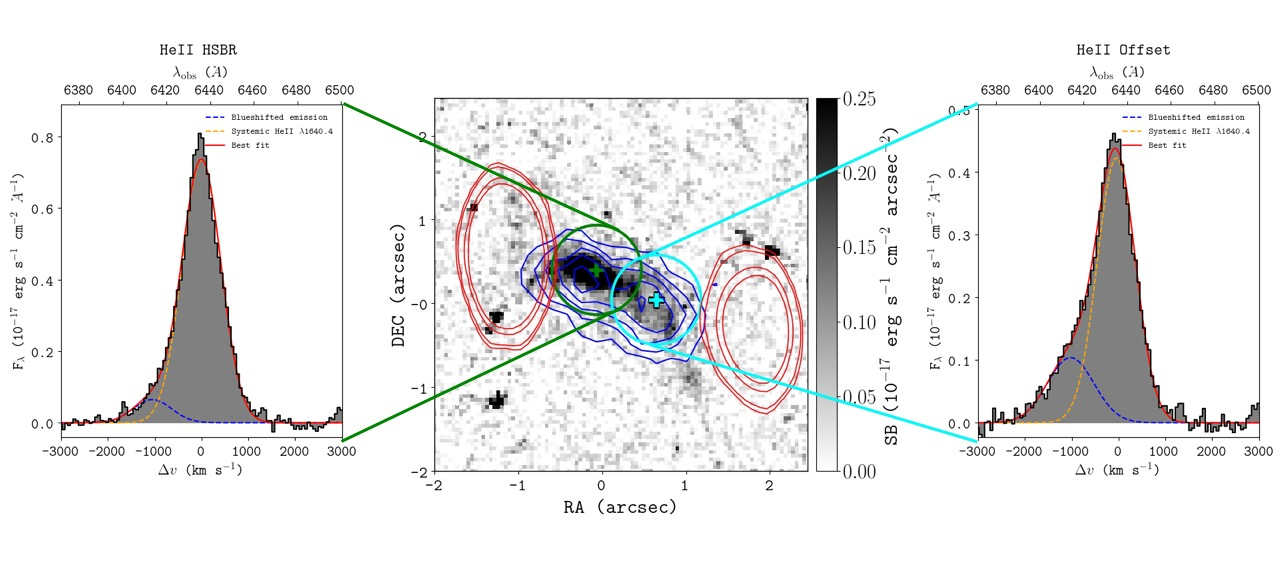
\includegraphics[width=1.2\textwidth]{plots_chp3/HeII_nucleus_offset_NB_img.jpg}
\caption[HST rest-UV image overlaid with MUSE \ion{He}{II} and VLA 4.7 GHz contours]{Broad-band image of the rest-UV continuum of MRC 0942-242 from the {\it HST} WFPC2 702W ($5800 - 8600$ $\ang$) filter. MUSE contours (blue) are overlaid and represent narrow-band emission summed over $6400 - 6425$ $\ang.$ The contours are shown at the surface brightness levels, (1.0, 1.6, 2.2, 2.8, 3.4, 4.0) $\times 10^{-17}$ erg s$^{-1}$ cm$^{-2}$ $ {\rm arcsec}^{-2}.$ VLA 4.7 GHz radio surface brightness is shown by the red contour levels. The inset 1D spectra show the HSBR ($left$) and offset ($right$) \ion{He}{II} emission. The line profiles are extracted from apertures of radius R = 0.6\arcsec, shown in green for the HSBR and in cyan for the offset region. The aperture centroids for each are shown in matching colours. The blueshifted and systemic \ion{He}{II} emissions are shown in blue and orange, respectively, and the sum of both components is shown in red. }
\label{fig:hst-img-muse-contours}
\end{figure*}

Obtaining a narrow-band image over a smaller wavelength range of $6400 - 6412$ $\ang$ (blue interval in Fig \ref{fig:0943-emission}(d)) allows us to distinguish the blueshifted \ion{He}{II} emission from the \ion{He}{II} emission at the systemic velocity. \ion{He}{II} emission from the blueshifted component alone is shown in Fig \ref{fig:0943-emission}(a), which proves that emission from the blue wing of the \ion{He}{II} line is indeed spatially offset from the HSBR.

\ion{The He}{II} emission at the systemic velocity is less highly concentrated. Over the green interval in Fig. \ref{fig:0943-emission}(d), \ion{He}{II} is diffuse and elongated well beyond the radio lobes, indicating possible jet-gas interactions. At the red wing of the line, \ion{He}{II} emission is concentrated in the eastern lobe and HSBR, as Fig. \ref{fig:0943-emission}(c) shows. 

Both \lya~and \ion{C}{IV} show evidence for turbulent blueshifted motions in the line-fitting (see sections \ref{section:Lya-fit} and \ref{section:CIV-NV-fit}). If the blueshifted component is indeed an outflow, this implies that the outflowing gas contains more than one ionised gas tracer, which we can expect for a bulk outflow of gas from the enriched ISM. 

\begin{sidewaystable}
\caption[Best-fit \ion{He}{II} emission line results]{Best-fit results to \ion{He}{II} HSBR and offset lines in Fig. \ref{fig:hst-img-muse-contours}. The emission is also classified as blueshifted relative to the systemic velocity or is emitted from the systemic velocity.}    
\centering                          
\begin{tabular}{ l l D{,}{\, \,\pm\, \,}{-3} D{,}{\, \,\pm\, \,}{-3} D{,}{\, \,\pm\, \,}{-3} D{,}{\, \,\pm\, \,}{-3} }
\hline\hline MUSE  \\
\hline            
\ion{He}{II}$\lambda1640$ line region  
& Component 
& \mc{Line centre (obs.)} 
&\mc{Line flux}  
& \mc{Line width}
& \mc{Velocity}   \\ 
&  
& \mc{$\lam$ (\ang)} 
& \mc{$F$ (10$^{-17}$ erg s$^{-1}$ cm$^{-2}$)}
& \mc{FWHM (km s$^{-1}$)} 
& \mc{$\Delta \varv$} \\  
&  &  & \mc{} & \mc{} &\mc{} \\  
\hline     
&  &  & \mc{} & \mc{} &\mc{} \\  
HSBR    & blueshifted   & 6413.49,3.04   & 1.43,0.47       & 970, 225       & -1053,3206  \\  
              & systemic       & 6436.09,0.30  & 16.42,4.86    & 978, 24         & 0.02,0.01 \\ 
&  &  & \mc{} & \mc{} &\mc{} \\                                  
Offset  & blueshifted     & 6414.18,3.21  & 2.69,0.81                & 1134, 195     & -1025,3251\\  
            & systemic        & 6434.76,0.83  & 7.64,0.80             & 993,48          & -46,27 \\   
&  &  & \mc{} & \mc{} &\mc{} \\   
\hline                                   
\end{tabular} 
\label{table:HeII-nucleus-offset}  
\end{sidewaystable}

\begin{figure}
\hspace*{-50pt}
\centering
        \subfloat[\ion{He}{II} blueshifted: $6400 - 6412$ $\ang;$ blue interval in Fig. \ref{fig:0943-emission}(d)]{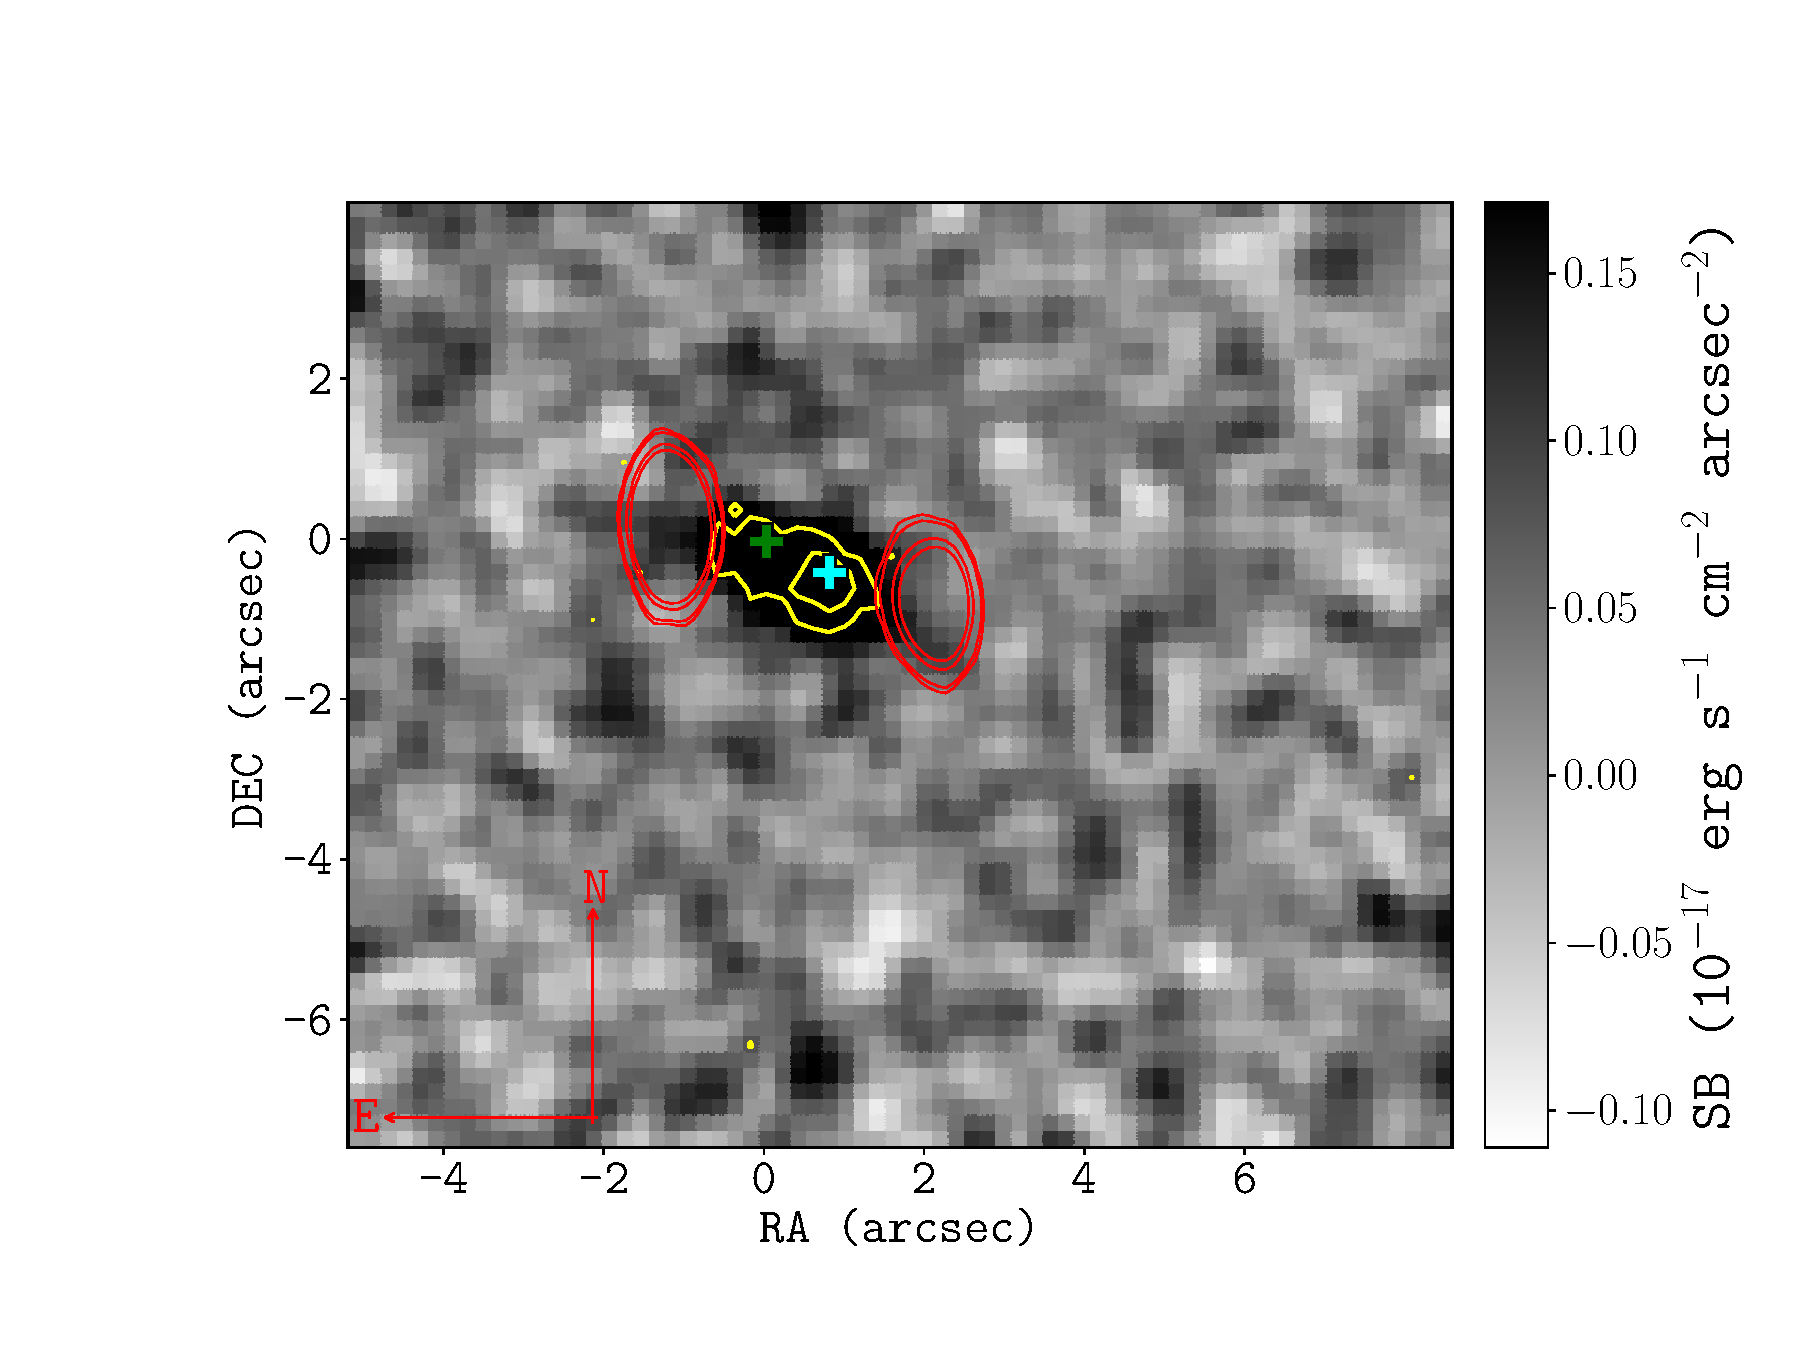
\includegraphics[width=0.6\textwidth]{plots_chp3/HeII_blue_VLA_arcsec.pdf}}
        \subfloat[\ion{He}{II} diffuse: $6425 - 6430$ $\ang;$ green interval in Fig. \ref{fig:0943-emission}(d)]{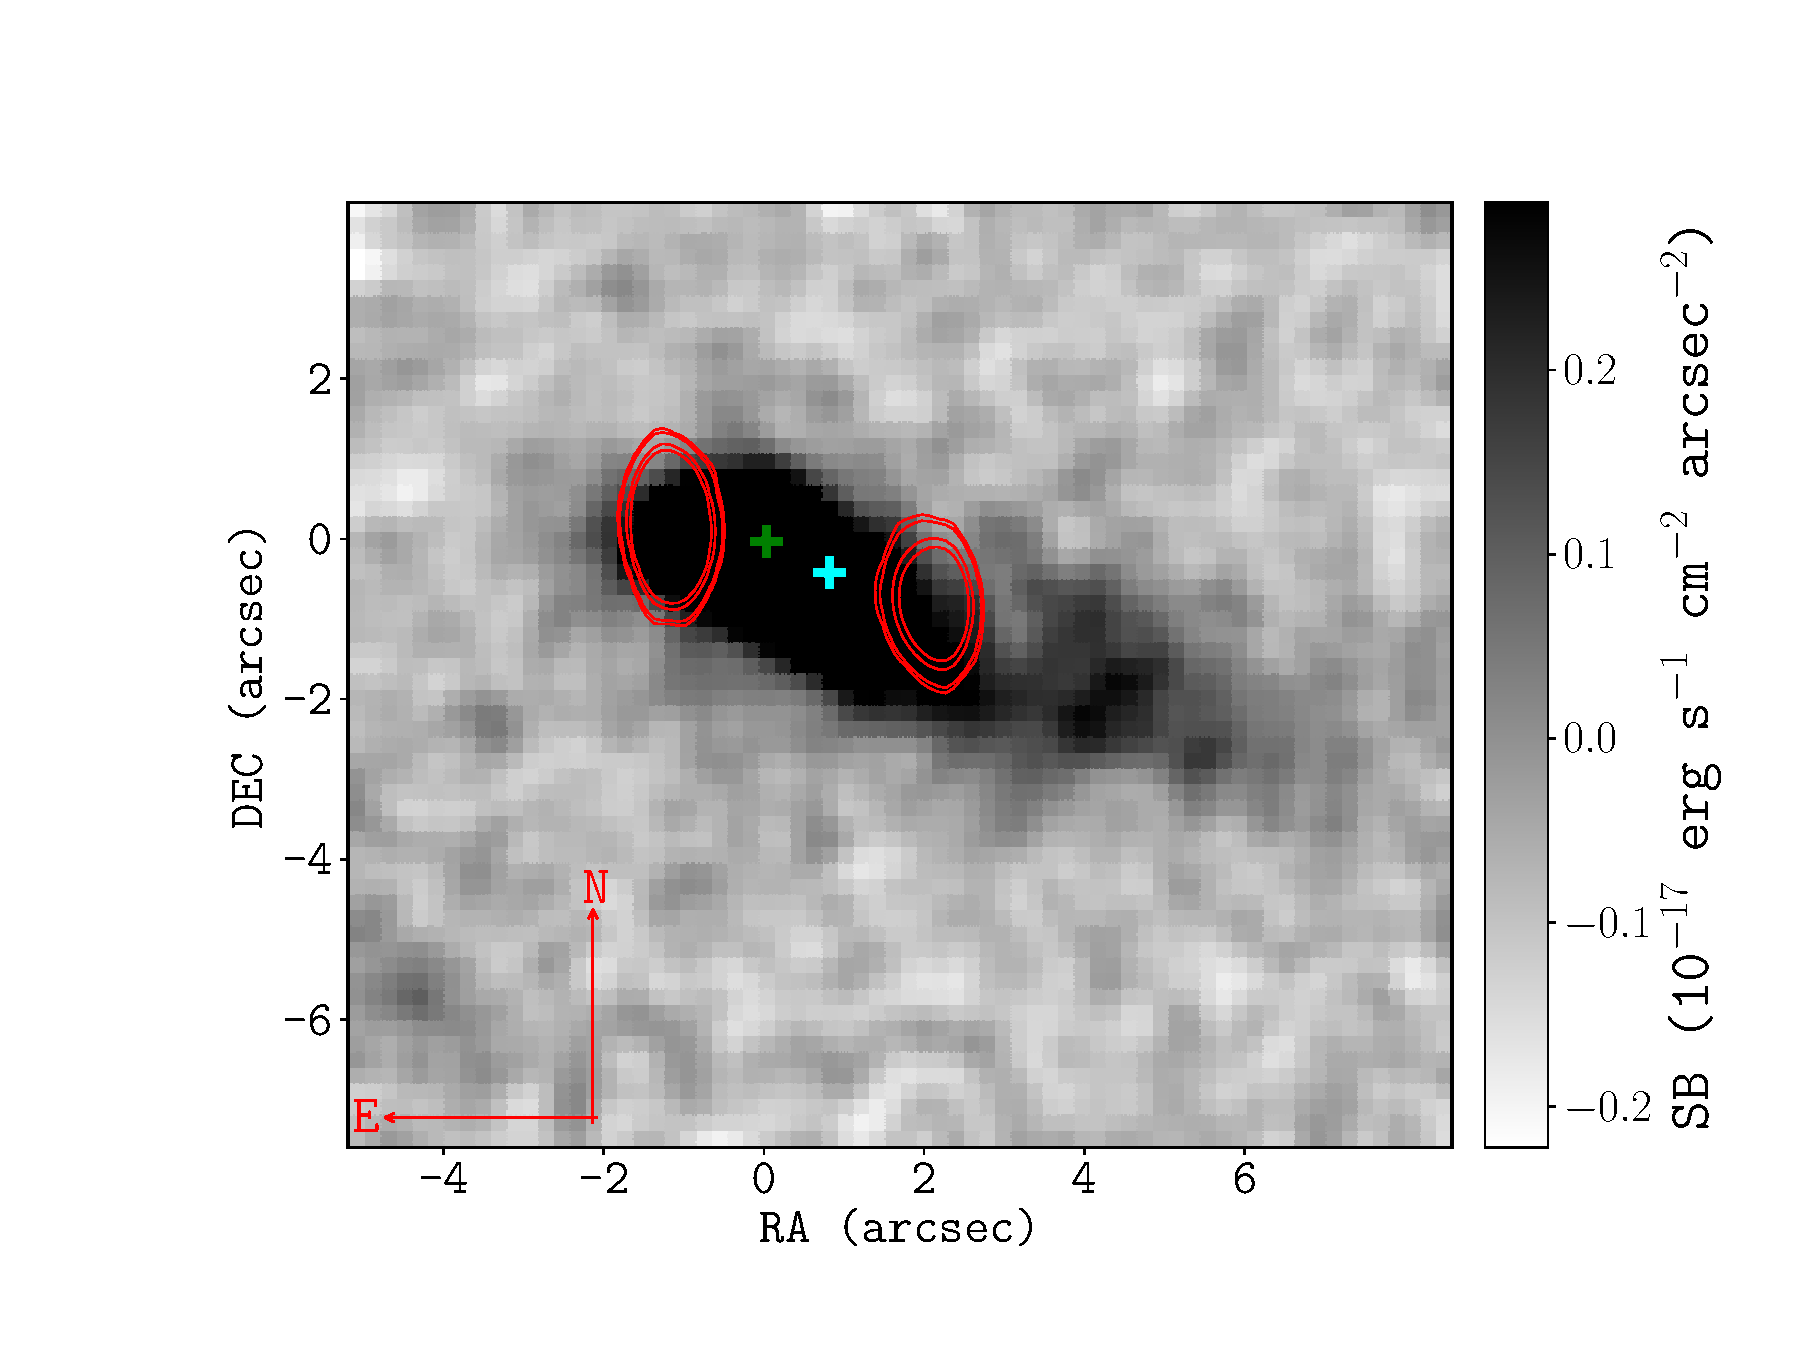
\includegraphics[width=0.6\textwidth]{plots_chp3/HeII_green_VLA_arcsec.pdf}}\\
\hspace*{-50pt}
        \subfloat[\ion{He}{II} redshifted: $6445 - 6450$ $\ang;$ red interval in Fig. \ref{fig:0943-emission}(d)]{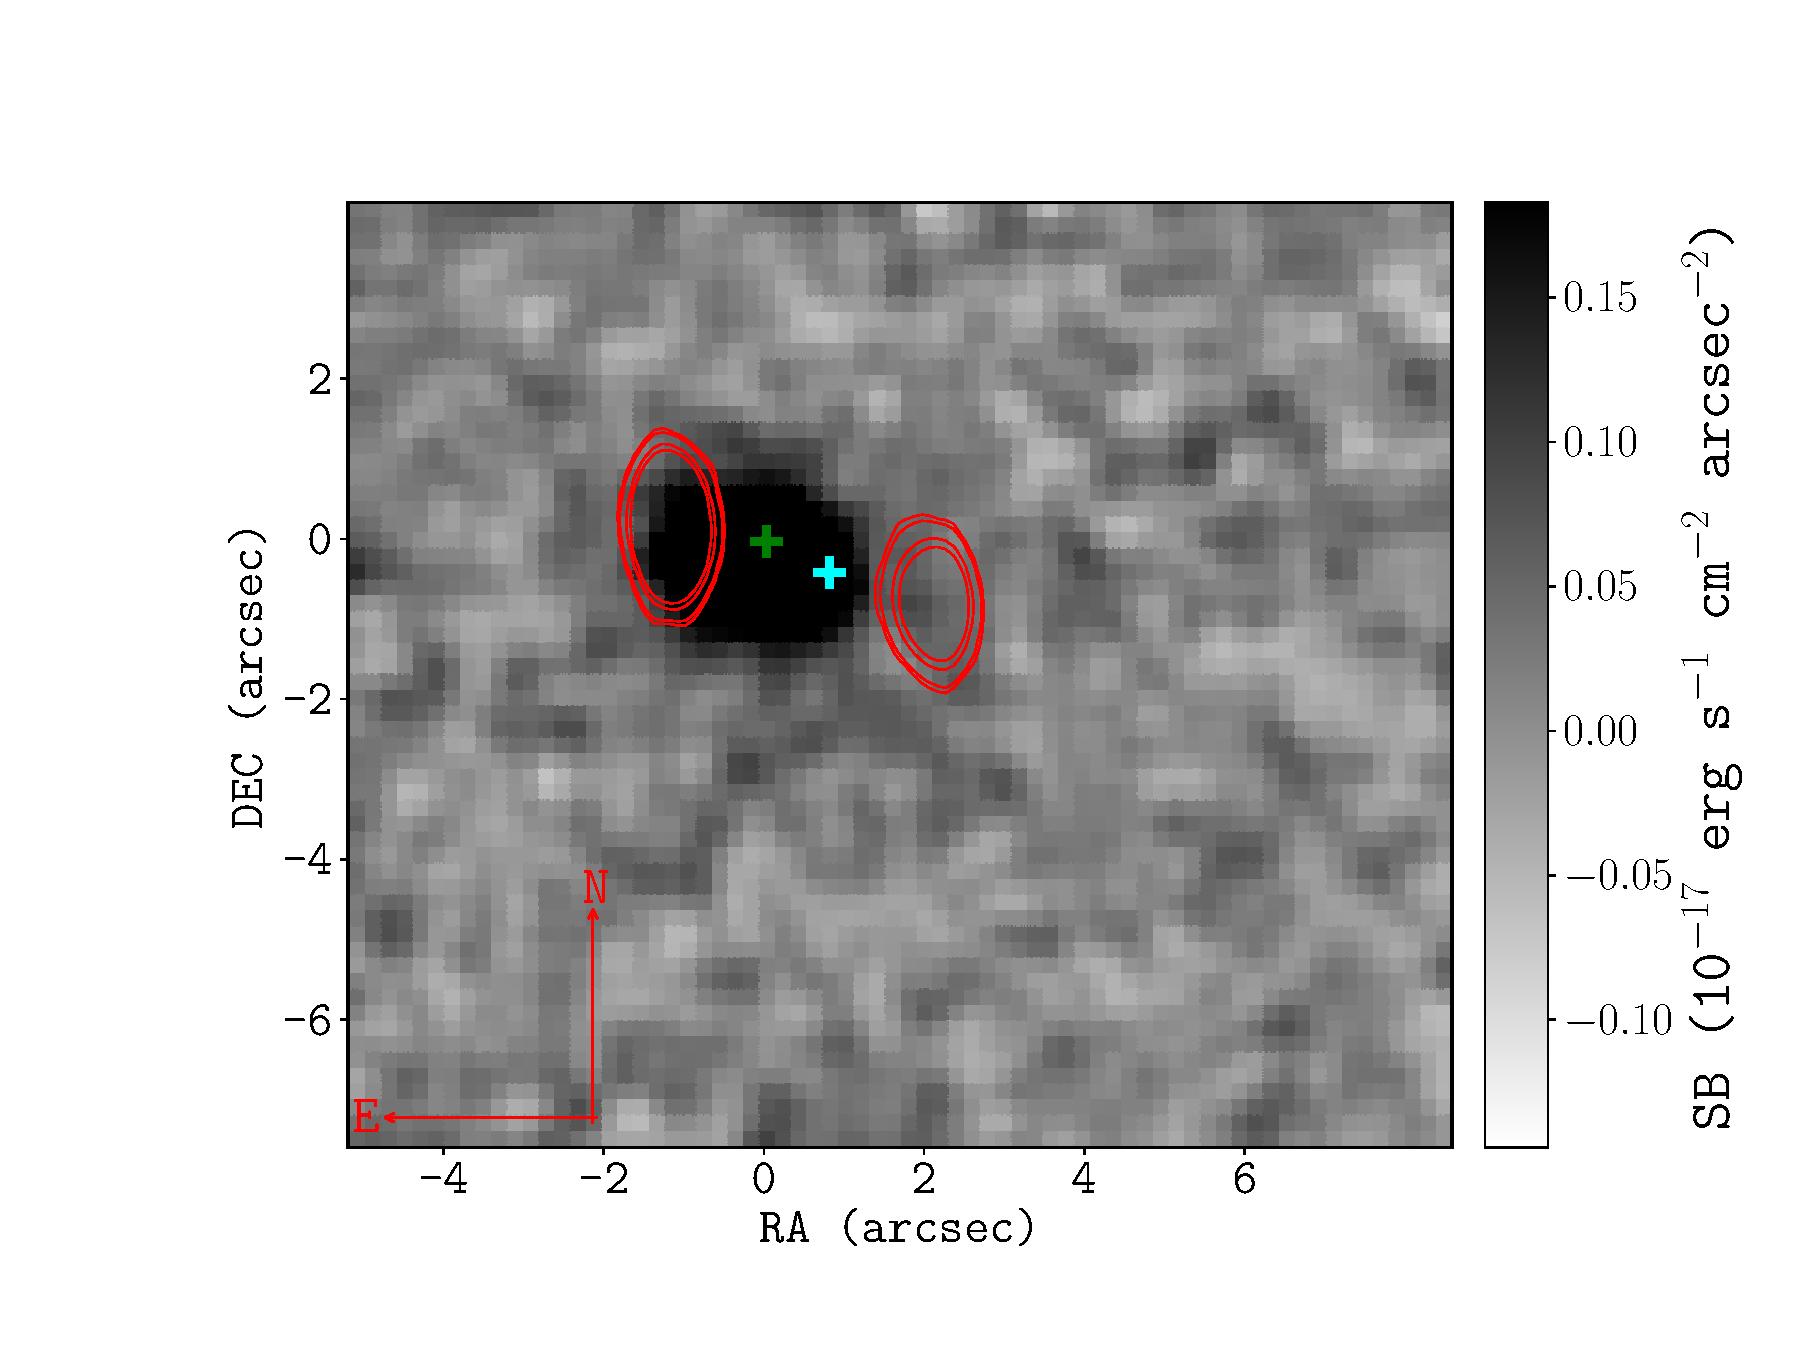
\includegraphics[width=0.6\textwidth]{plots_chp3/HeII_red_VLA_arcsec.pdf}}
        \subfloat[\ion{He}{II} line emission]{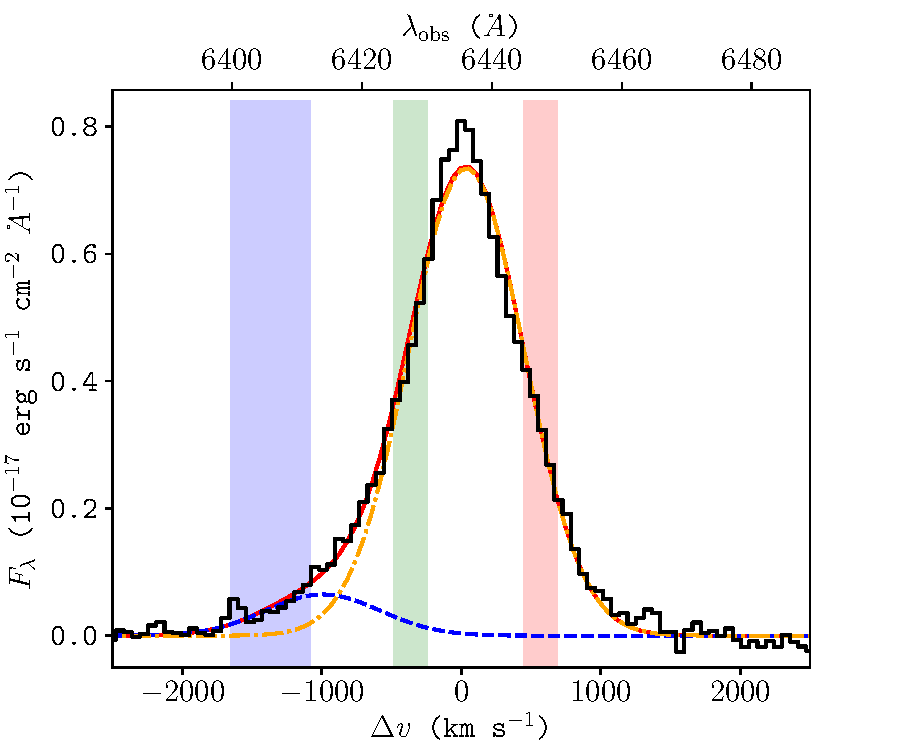
\includegraphics[width=0.5\textwidth]{plots_chp3/HeII_profile.pdf}}
\caption[MUSE \ion{He}{II} narrow-band images]{MUSE continuum-subtracted narrow-band images showing the spatial variation in \ion{He}{II} emission at different wavelength bands. The green and cyan crosses show the centres of the HSBR and offset \ion{He}{II} emission from which the line profiles in Fig. \ref{fig:hst-img-muse-contours} are extracted. The 4.7 GHz VLA radio contours are shown in red at the levels $3\sigma,$ $3\sqrt{2}\sigma,$ $9\sqrt{2}\sigma,$ and $15\sqrt{2}\sigma$ for $\sigma = 2\e{-5}$ Jy beam$^{-1}$. Panel (a): The blueshifted component is detected over $6400 - 6412$ $\ang$ in the blue interval and is shown as a narrow-band image. In this figure, the sub-structure of the emission is also shown using MUSE \ion{He}{II} contours with surface brightness levels (0.038, 0.079, 0.120) $\times 10^{-17}$ erg s$^{-1}$ cm$^{-2} {\rm arcsec}^{-2}$ in yellow. Panel (b): The diffuse \ion{He}{II} gas, represented by the green spectral range, that is, $6425 - 6430$ $\ang,$ extends in the direction of the south-western lobe. Panel (c): In the red spectral interval, that is, $6445 - 6450$ $\ang,$ a redshifted component that has a clear spatial association with the north-eastern radio lobe is visible. The velocity intervals for these narrow-band images are displayed in the \ion{He}{II} profile in Panel (d), which is a spectrum extracted from an aperture centred on the HSBR over a radius of R = 0.6\arcsec. }
\label{fig:0943-emission}
\end{figure}

\section{Quasar and HzRG absorbers, in comparison}\label{section:hzrg-vs-quasar-abs}
The absorption lines in a quasar continuum emerge from absorption by intervening gas in the IGM and the CGM of a foreground galaxy \citep[e.g.][]{bechtold2001}. Here,we used quasar absorption lines to determine whether the absorbers in Yggdrasil are associated with the halo of the galaxy or the IGM, assuming that HzRG and quasar absorbers are drawn from the same parent population. 

To do this, we compared our results to quasar absorption parameters of \ion{H}{I}, \ion{N}{V,} and \ion{C}{IV} for associated quasar absorbers from \citet{fechner2009}. In this work, the absorbing gas identified as intervening is located at velocity shifts of $\lvert \Delta \varv \rvert > 5000$ km s$^{-1}$ from the quasars in their sample. The  associated absorbers are those at velocity shifts $\lvert \Delta \varv \rvert > 5000$ km s$^{-1}$ from the quasars. We show this comparison in Fig \ref{fig:NV-quasar-absorption}. Our results (which generally have velocity shifts $\lvert \Delta \varv \rvert < 1500$ km s$^{-1}$ for all absorbers) agree better with absorption by associated than by intervening gas. This implies that the absorbers in Yggdrasil are more likely to be associated with the galaxy, that is, the absorbers are bound to the ISM and/or CGM if they are similar or from the same parent distribution.

We have an additional set of quasar absorbers with which to compare the \ion{C}{IV} and \ion{Si}{IV} column densities we measured. Quasar absorption for the ionised gas, in particular, has been measured by \citet{songaila1998} and \citet{dodorico2013}. In the former, absorption is from the IGM, while the latter results show quasar-associated absorption at much higher redshifts of z $>$ 6. This comparison is shown in Fig. \ref{fig:SiIV-quasar-absorption}. This figure shows that Yggdrasil absorbers agree better with the associated absorbers of \citet{dodorico2013} than with the intervening absorbers of \citet{songaila1998}. These order-of-magnitude comparisons show that the absorbers in the Yggdrasil spectrum are much more likely to be associated with the galaxy halo.

\begin{figure} 
\captionsetup[subfigure]{labelformat=empty}
\hspace{1pt}
\centering
\subfloat[Comparison with associated quasar absorption]{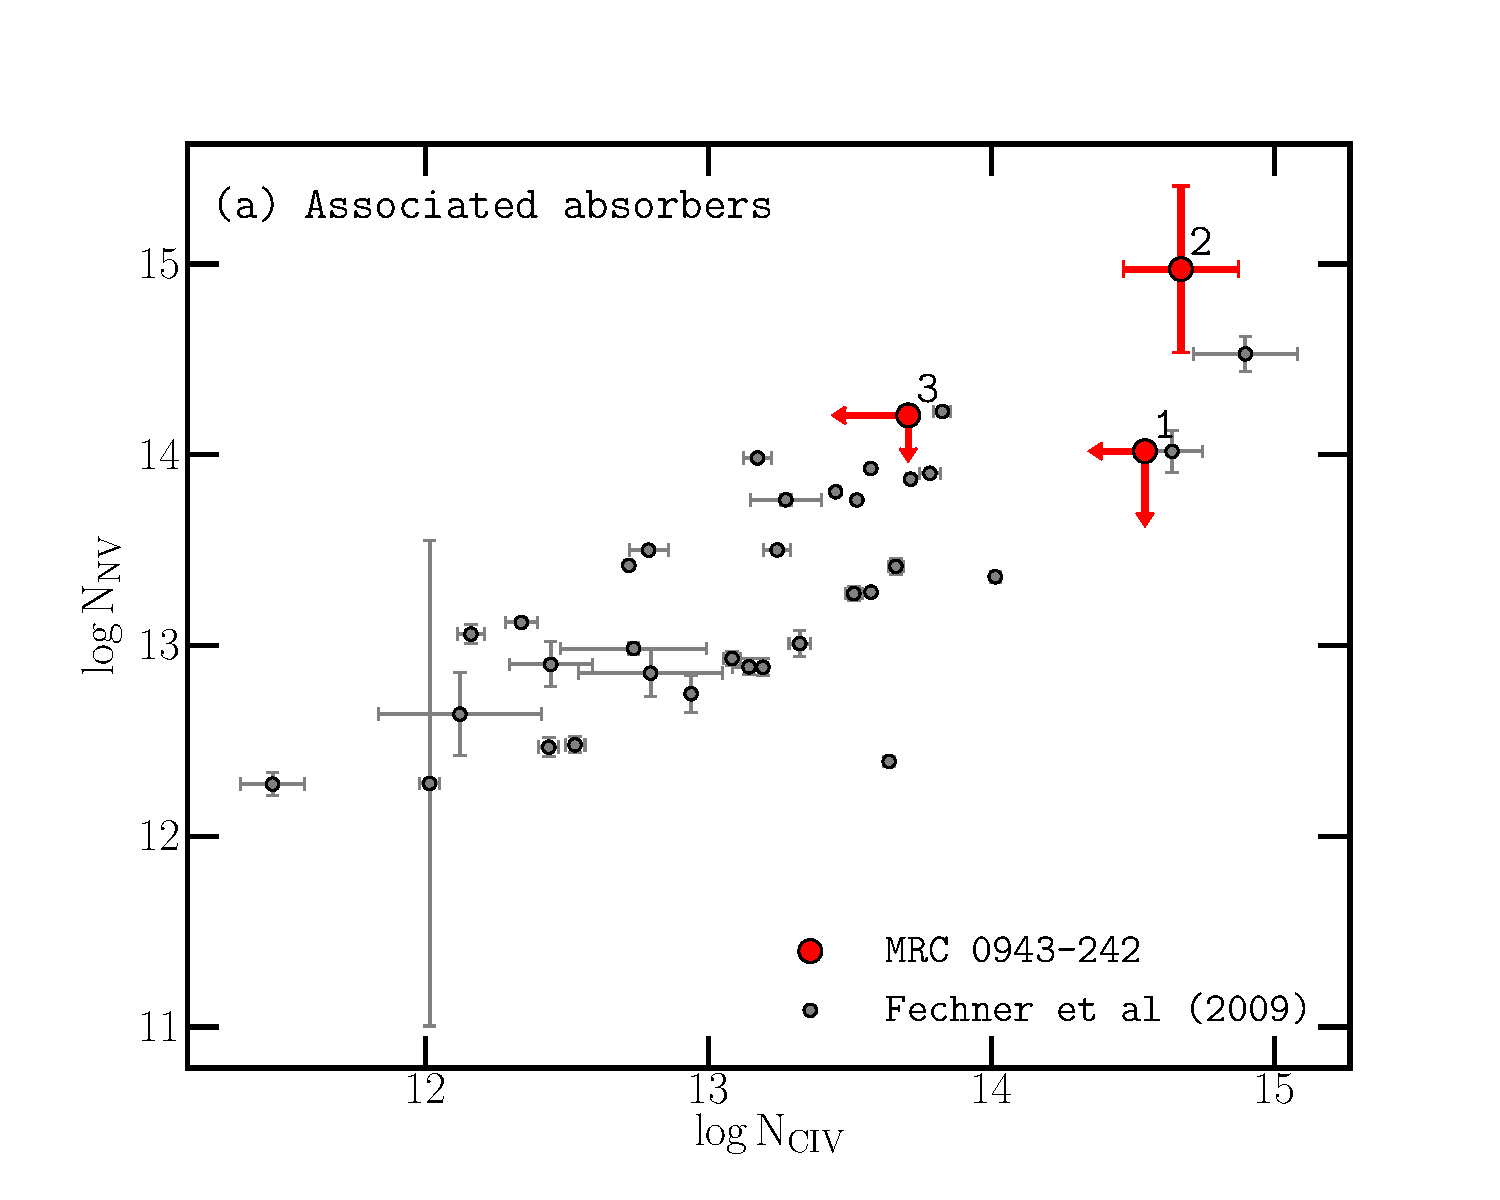
\includegraphics[width=0.55\textwidth]{plots_chp3/NV_associated_QSO_HzRGs.pdf}}
\centering
\subfloat[Comparison with intervening quasar absorption]{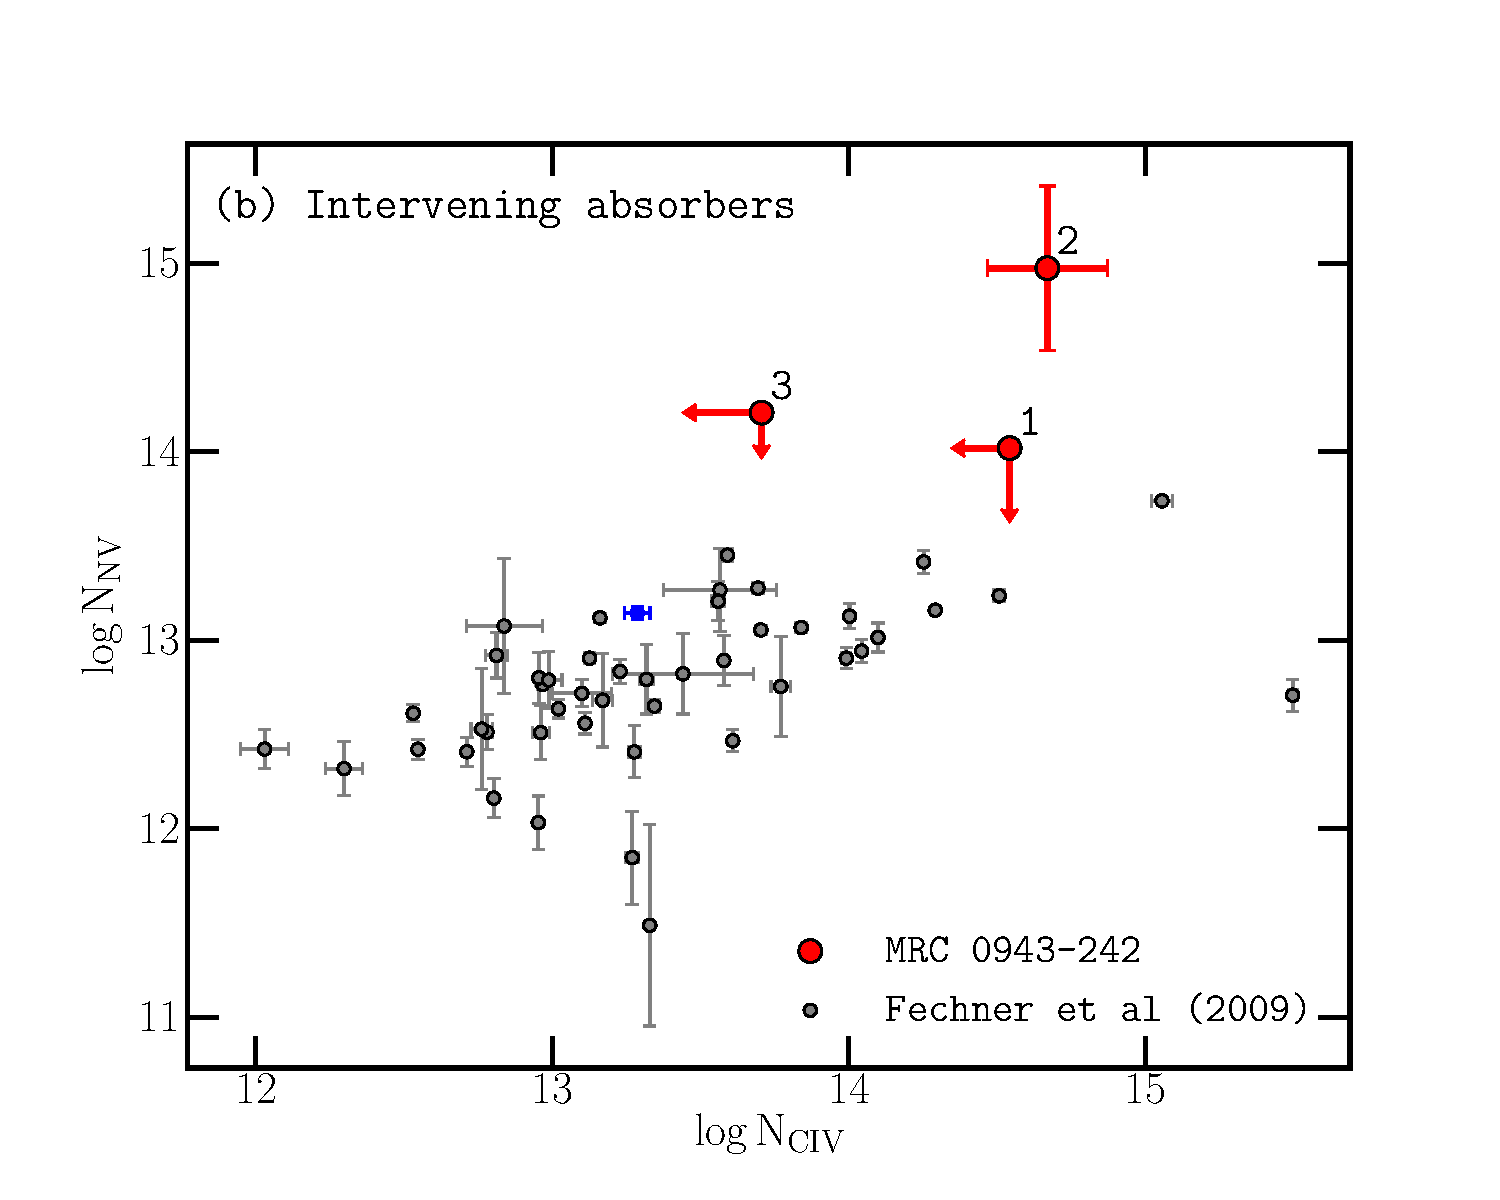
\includegraphics[width=0.55\textwidth]{plots_chp3/NV_intervening_QSO_HzRGs.pdf}}
\caption[$N_\ion{C}{IV}$ and $N_\ion{N}{V}$ column densities of host galaxy and quasar absorbers]{\ion{N}{V} and \ion{C}{IV} column densities of associated (left) and intervening (right) absorbers from \citet{fechner2009} (in grey and blue: secondary detections for the quasar) and Yggdrasil detections (red).}
 \label{fig:NV-quasar-absorption}
\end{figure}

\begin{figure} 
\centering
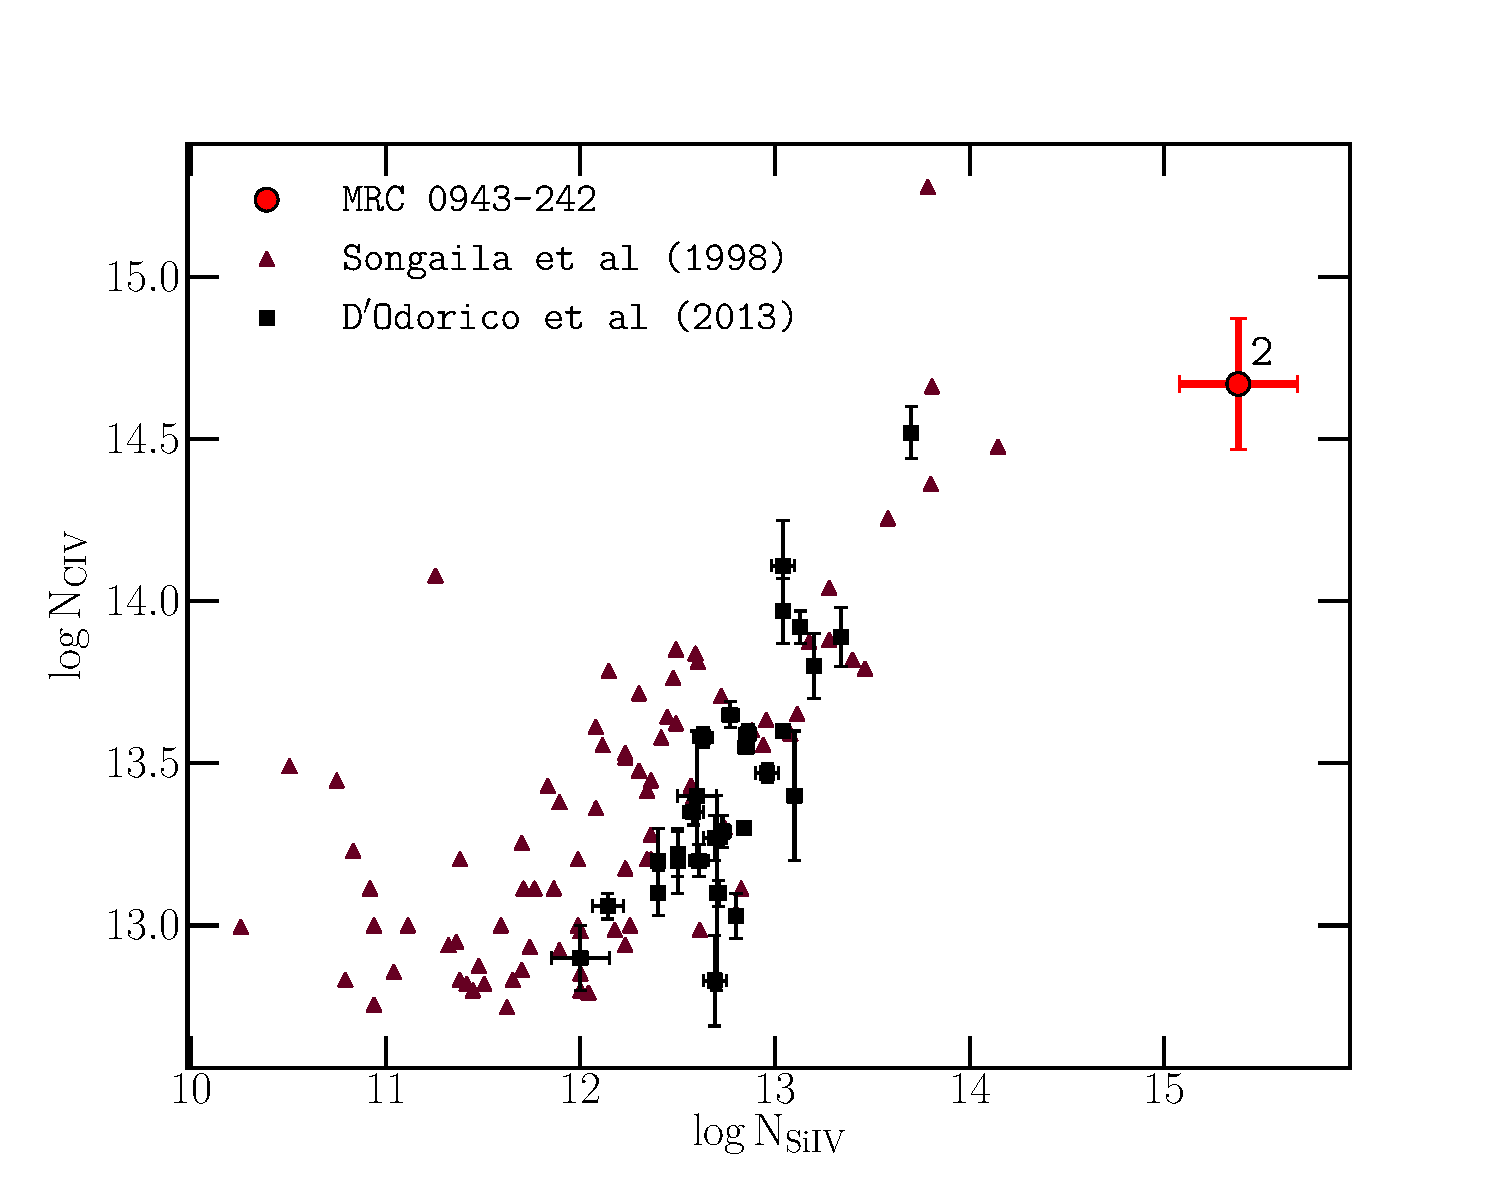
\includegraphics[width=0.55\textwidth]{plots_chp3/SiIV_CIV_QSO_HzRGs.pdf}
\caption[$N_\ion{C}{IV}$ and $N_\ion{Si}{IV}$ column densities of host galaxy and quasar absorbers]{$N_\ion{C}{IV}$ relative to $N_\ion{Si}{IV}$ for absorbers in the IGM in \citet{songaila1998} and those directly associated with the quasars \citep{dodorico2013}.}
\label{fig:SiIV-quasar-absorption}
\end{figure}

\section{Photoionisation modelling}\label{section:photoionisation-modelling}
We used a photoionisation modelling code to determine the main ionising mechanisms that produce the observed ionised gas and its column densities in the absorbing gas shells surrounding Yggdrasil. A very detailed study of this has been carried out by \citet{binette2000}, who obtained a metallicity of Z/Z$_\odot \simeq 0.02$ (Z$_\odot$ being the solar metallicity) for the strongest \lya~absorbers. Their findings also indicated that emitting and absorbing gas are not co-spatial and that the gas is best described by an \ion{H}{I} volume density of n$_\ion{H}{I} = 100$ cm$^{-3}.$ In addition to this, \citet{binette2006} sought to determine the ionising mechanism behind the absorbers in this source, and thus showed that stellar photoionisation results in the \ion{H}{I} and \ion{C}{IV} absorber column densities 

It is worth noting that their conclusions were obtained using only column densities for \ion{H}{I} and \ion{C}{IV}. With our recent detection of \ion{N}{V} absorption at the same velocity as the the strong \lya~absorber, we can provide more insight to these findings. Given the detection of \ion{N}{V}, flux from the meta-galactic background may be too weak to ionise the absorbers. At z $\geq$ 2.7, \ion{He}{II} reionisation was more active than it is at lower redshifts, meaning that ionising photons with energies of $E_\gamma > 54.4$ eV had megaparsec-scale mean free paths \citep{shull2010,mcquinn2016}. The meta-galactic background is therefore less likely to be a strong ionising mechanism powering the absorbers in the halo of Yggdrasil. 

We also considered the possibility that shocks by the powerful radio jets may ionise the gas. This was proposed by \citet{dopita1995}, and observational evidence for shock ionisation in HzRGs has been shown by several authors, particularly in sources with relatively small radio sources that are still contained within the host galaxy \citep[e.g.][]{allen1998,best2000a,debreuck2000}. A powerful diagnostic of shock-ionised emission are the line ratios of carbon: in shock ionised regions, we expect the \ion{C}{II]} $\lam2326$ line to be as strong as its higher ionisation counterparts. Our MUSE spectrum (Fig. \ref{fig:0943-spectrum}) contains three carbon lines and allows us to make this test. Interestingly, the \ion{C}{II]} $\lam1906,1908$ line contains a much stronger blueshifted component than the \ion{C}{III]} and \ion{C}{IV} $\lam\lam1548,1550$ lines. These high \ion{C}{II]}/\ion{C}{III]} and \ion{C}{II]}/\ion{C}{IV} ratios are consistent with shock ionisation \citep[see e.g. Fig. 1 of][]{best2000a}. This provides evidence to our claim that this blueshifted gas near the western radio lobe is an outflow driven by the radio jet. On the other hand, the radio of the main component near the AGN has a \ion{C}{III]}/\ion{C}{II]} ratio of $\sim$2.4, which places it squarely in the AGN photoionisation region. This main velocity component dominates the flux of all the other emission lines, therefore we did not consider shock ionisation as a relevant contributor in those lines.

Stellar photoionisation is a possibility as well. The star formation rate (SFR) in Yggdrasil, however, is SFR=41 M$_\odot$ yr$^{-1}$ \citep{falkendal2019} and may be insufficient to produce the starburst activity that would ionise the absorbers. Another possibility is the AGN, which we can expect to produce a strong enough ionising continuum to produce the detected absorption. 

We therefore revisited the analysis by running photoionisation models using \pkg{cloudy c17} \citep{ferland2017}, a spectral synthesis code designed to run grid models that provide simulated chemical abundances in photoionised gas. Within the halo of Yggdrasil, we have shown that \lya~absorbers are at the same velocity as \ion{C}{IV}, \ion{N}{V,} and \ion{Si}{IV} absorbers, suggesting that the gas tracers occupy the same gas volume. 

The ionisation parameter is defined as $U(r) = \frac{ 1 }{ 4 \pi {\rm r}^2 {\rm c} {\rm n}_\ion{H}{I}} \int^\infty_{\nu_0} \frac{ {\rm L}_\nu }{ h\nu }d\nu,$ is the quotient of the volume density of hydrogen-ionising photons and the volume density of hydrogen atoms contained within the gas. Here, $r$ is the line-of-sight distance from the ionising source to the gas, n$_\ion{H}{I}$ is the hydrogen density, $L_\nu$ is the specific luminosity, and $\nu$ is the observing frequency such that the integral, $\int^{\infty}_{\nu_0} \frac{ {\rm L}_\nu }{ h\nu }d\nu,$ is the luminosity of the ionising source. Provided that we can determine $U(r)$ for the radiation field ionising the absorbing gas, we can also compute the distance of the gas from the radiation source  along the line of sight.

\subsection{AGN photoionisation of the absorbers}\label{section:photoionisation-absorbers}

We have shown in the comparison to quasar absorbers in \citet{fechner2009} that the absorbers in Yggdrasil are located within the CGM rather than IGM. In the \pkg{cloudy} model, we used a power law spectral energy distribution \pkg{(SED;} where the ionising flux is given by S$_\nu \propto \nu^\alpha$) to simulate the incident radiation produced by the AGN. In this, we tested $\alpha=-1.5$ and $\alpha=-1.0$ to model the photoionisation of the gas by an AGN \citep[e.g.][]{villar-martin1997,feltre2016,humphrey2018}.

The model grid consists of a set of input parameters. The hydrogen density was fixed to n$_\ion{H}{I} = 100 {\rm cm}^{-3}$ , which is commonly adopted to describe the low-density diffuse gas that we expect in the extended absorbers \citep[e.g.][]{binette2000,humphrey2008a}. The metallicity (Z) was varied over a range of values between Z/Z$_\odot$ = 0.01 and 10. The \ion{H}{I} column density N$_\ion{H}{I}$ was taken from the line-fitting results (shown in Table \ref{table:absorption-fits}). The ionisation parameter varied over the range $ 10^{-2.5} < U < 10^{-1}$ in 0.5 dex increments.

We did not include the effects of dust extinction because the surface brightness of emission re-radiated by dust, detected by the Atacama Large Millimetre/sub-mm Array (ALMA) at an observing frequency of $\nu_{\rm obs}$ = 235 GHz is lower in Yggdrasil than in the offset region at projected distances of $d = 65$ to 80 kpc from the host galaxy, where three resolved dusty companions are observed (G16). This observation implies that dust has a negligible contribution to the \pkg{SED} at the host galaxy. Moreover, \citet{falkendal2019} have shown that the SFR in Yggdrasil is lower than that which is detected in the companion sources, collectively. 

In the \pkg{cloudy} models, we have assumed an open or plane-parallel geometry for the absorbing gas medium, which implies that the cloud depth is significantly smaller than its inner radius, or more simply, the distance between the ionising continuum source and the illuminated gas surface. Following the findings from \citet{binette2000}, we assumed that the absorbers are not co-spatial with the emitting gas. 

The column density measures we obtain are shown against the simulated column densities in Figs. \ref{fig:cloudy-abs1} and \ref{fig:cloudy-abs3}, and the results indicate that absorbers 1 and 3 may have supersolar metallicities of Z/Z$_\odot \simeq$ 10 and 5, respectively. However, due to uncertainties in line-fitting, the column densities obtained are upper limits and no proper conclusion can be drawn about the metallicities of the absorbers. If these models were to suggest super-solar metallicity in absorbers, this would not be unusual given that super-solar metallicities in HzRG absorption line gas have been measured before \citep{jarvis2003,binette2006}. \citet{jarvis2003} showed that absorbers in the halo of the z=2.23 radio galaxy, 0200+015, had Z/Z$_\odot \sim$ 10 and covering factors of C $<$ 1.0. This implied that the absorbers are likely to be co-spatial with the EELR. Based on Fig. \ref{fig:cloudy-abs2}, the measured column densities of absorber 2 prove that its metallicity is closer to a value of Z/Z$_\odot = 0.01.$  The results also suggest that the \ion{N}{V} column density is under-predicted by the Z/Z$_\odot = 0.01$ model. We explore the possible reasons for this in the following section. 

\begin{figure}
\centering 
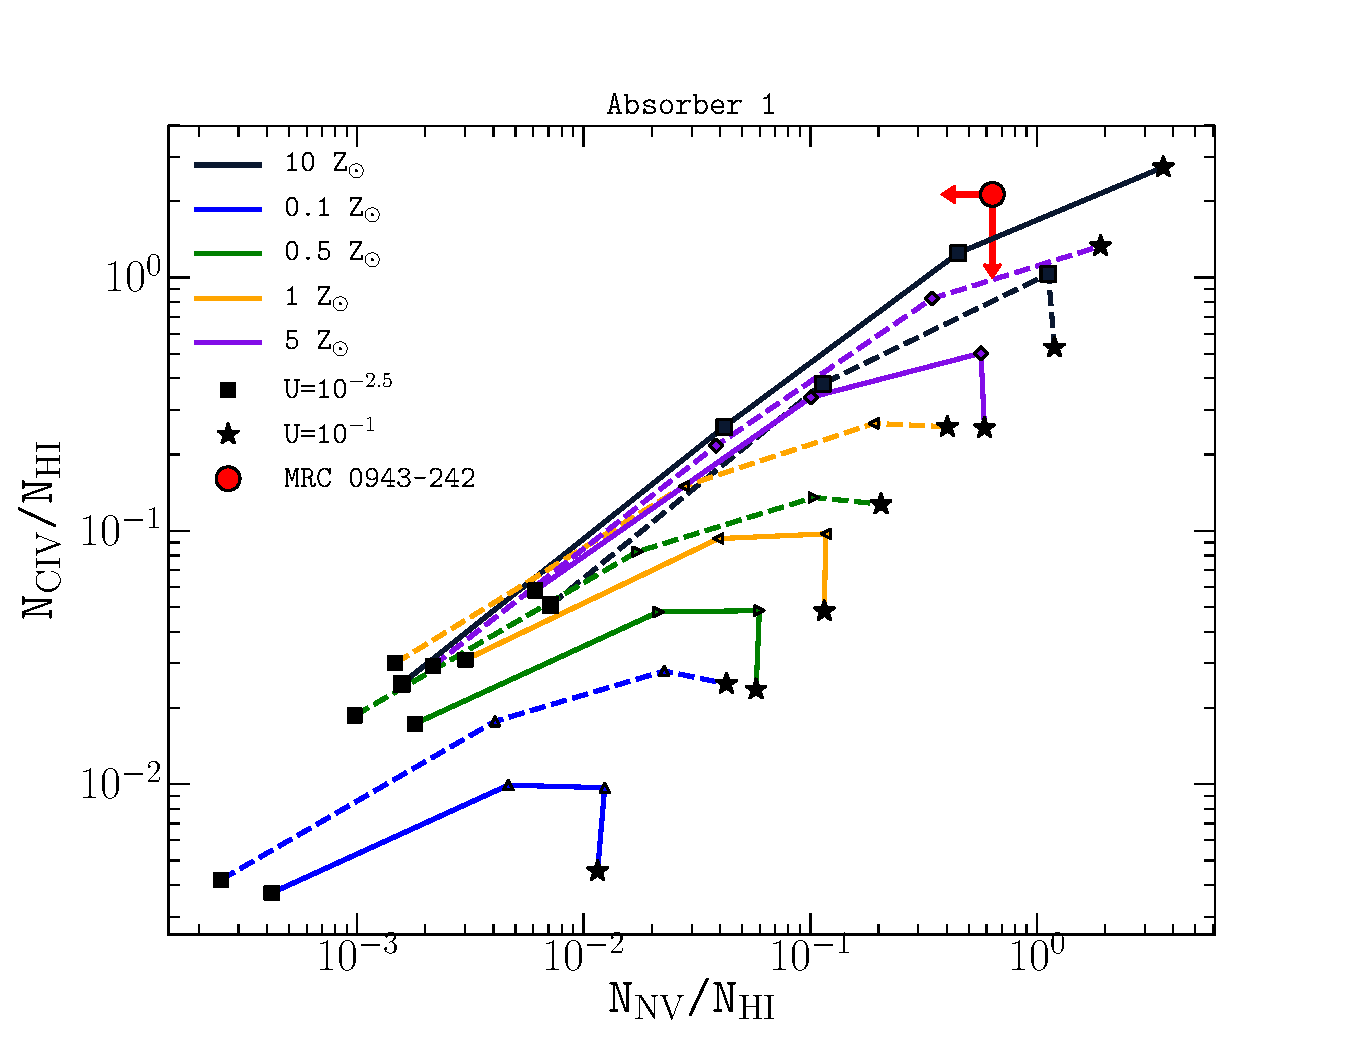
\includegraphics[width=0.7\textwidth]{plots_chp3/0943_agn_photoion_CIV_NV_HI_abs1_hden_2.pdf}
\caption[Absorber 1: \pkg{cloudy} photoionisation predictions]{\ion{N}{V} and \ion{C}{IV} column densities obtained from \pkg{cloudy} photoionisation models. The predicted column densities are for absorber 1, which has an \ion{H}{I} column density of $N_{\ion{H}{I}} = 10^{14.2}$ cm$^{-2}$ that is kept constant as $U(r)$ increases from $U=10^{-2.5}$ to $U=10^{-1}$ in increments of 0.5 dex. The metallicities Z/Z$_\odot$ = 0.1, 0.5, 1, and 5 are tested for spectral indices $\alpha=-1.0$ (solid lines) and $\alpha=-1.5$ (dashed lines).}
\label{fig:cloudy-abs1}
\end{figure}

\begin{figure}
\centering
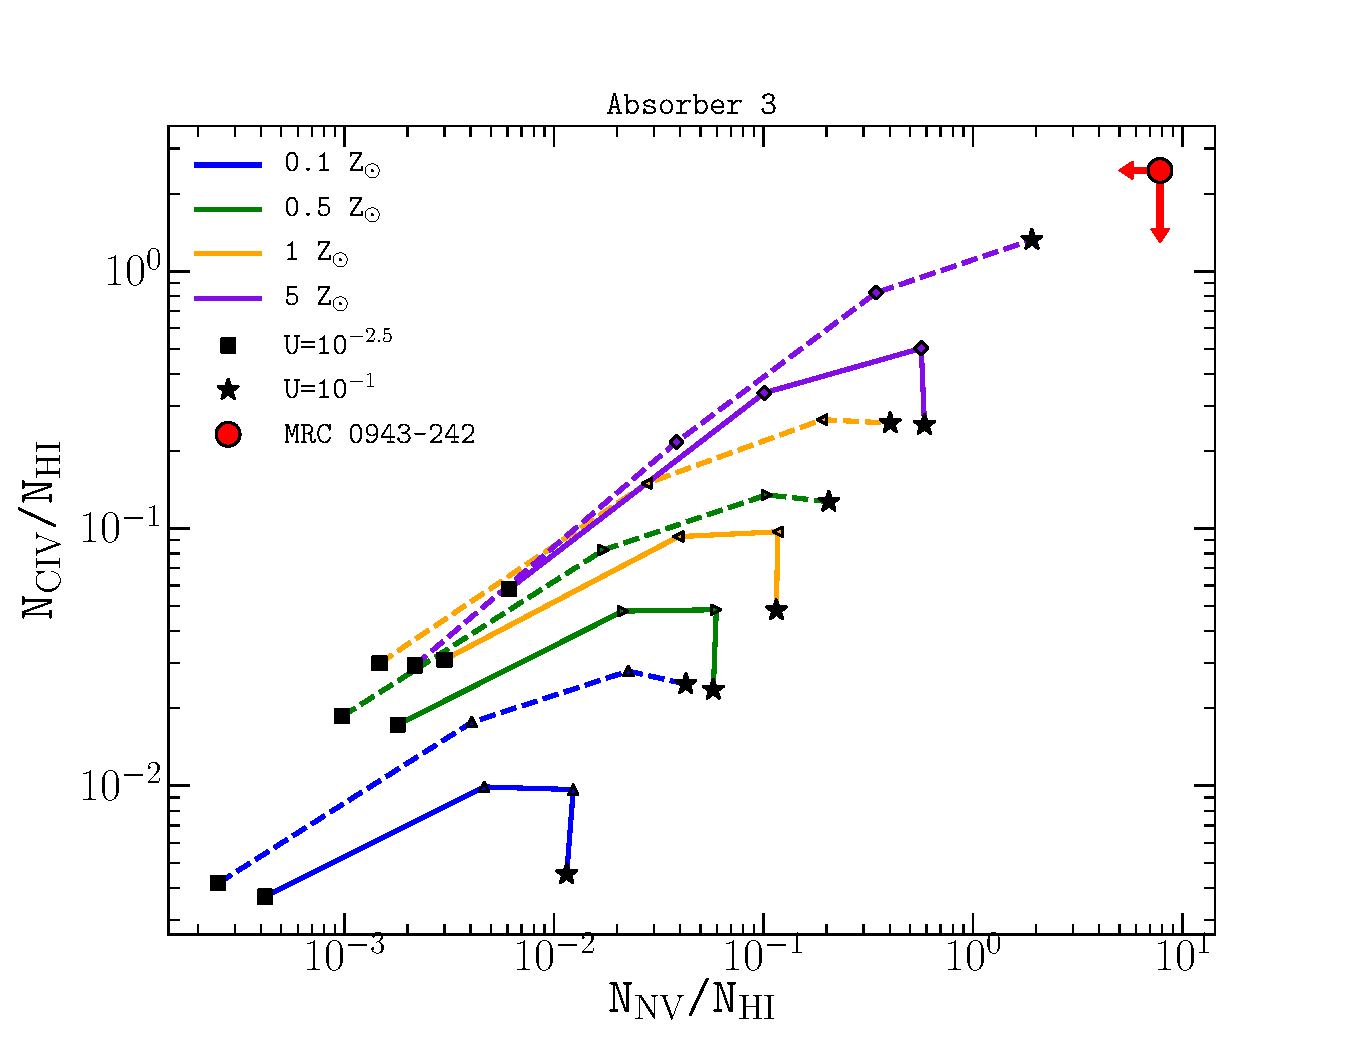
\includegraphics[width=0.7\textwidth]{plots_chp3/0943_agn_photoion_CIV_NV_HI_abs3_hden_2.pdf}
\caption[Absorber 2: \pkg{cloudy} photoionisation predictions]{\ion{N}{V} and \ion{C}{IV} column densities obtained from \pkg{cloudy} photoionisation models similar to those in Fig \ref{fig:cloudy-abs1}. The models shown here are for absorber 3 because the \ion{H}{I} column density is kept constant at $N_{\ion{H}{I}} = 10^{13.3}$ cm$^{-2}.$ The metallicities tested are Z/Z$_\odot$ = 0.1, 0.5, 1, and 5.}
\label{fig:cloudy-abs3}
\end{figure} 

\begin{figure}
\centering
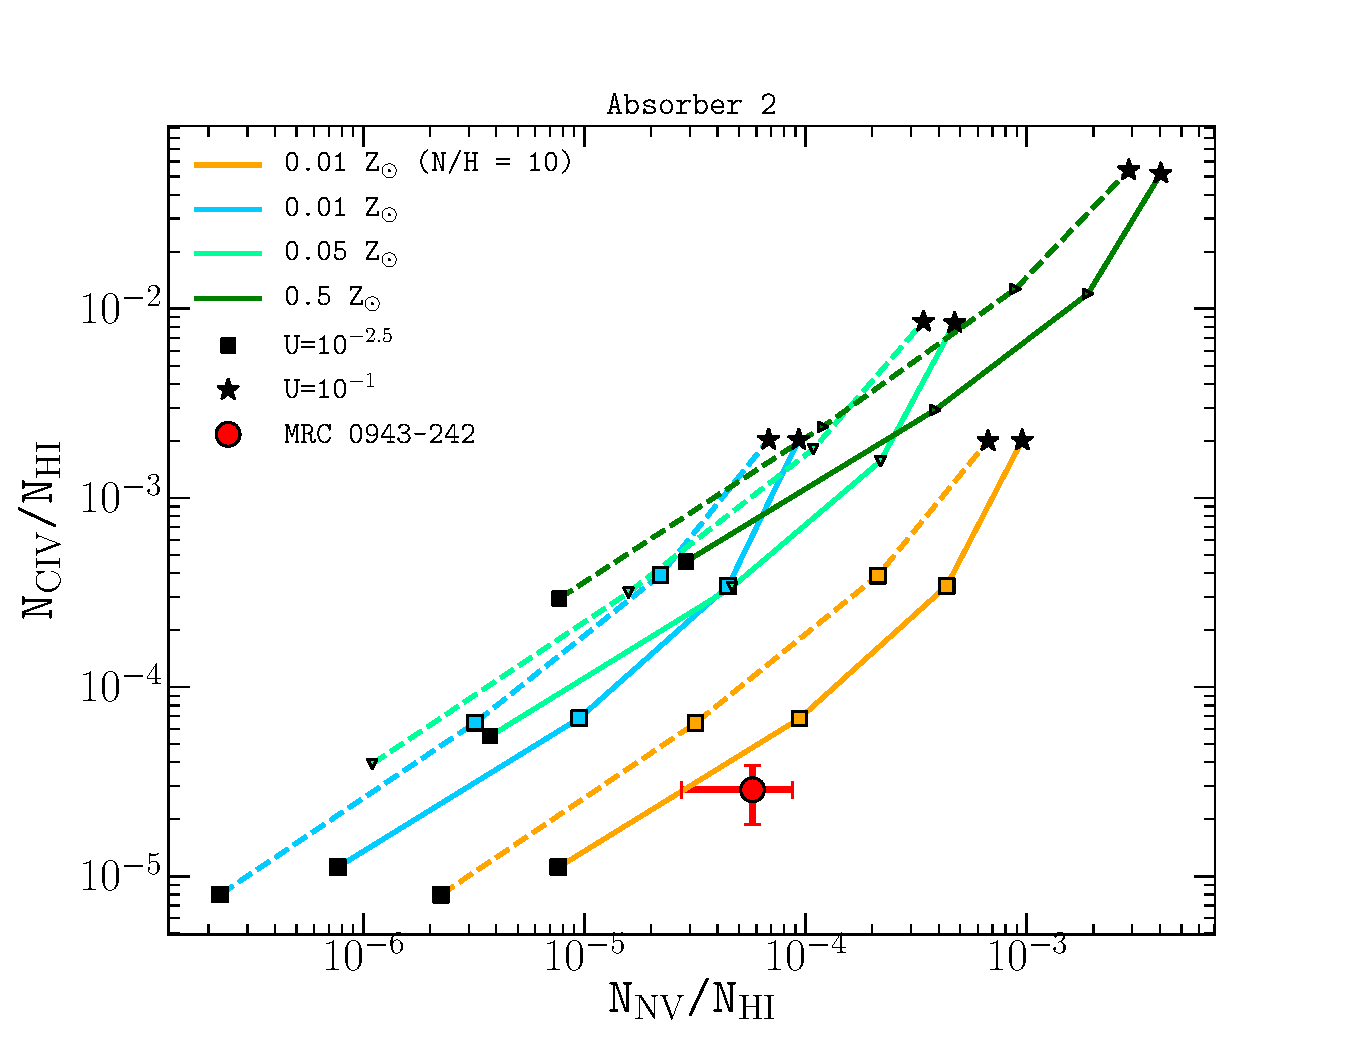
\includegraphics[width=0.7\textwidth]{plots_chp3/0943_agn_photoion_CIV_NV_HI_abs2_hden_2.pdf}
\caption[Absorber 3: \pkg{cloudy} photoionisation predictions]{\ion{N}{V} and \ion{C}{IV} column densities obtained from photoionisation \pkg{cloudy} models similar to those in Fig. \ref{fig:cloudy-abs1}. The models shown here are for absorber 2, the strong absorber, because the \ion{H}{I} column density is kept constant at $N_{\ion{H}{I}}$ = $10^{19.2}$ cm$^{-2}.$ The nitrogen abundance at Z/Z$_\odot = 0.01$ has also been enhanced by a factor of 10 (orange curve) i.e. N/C = 10.}
\label{fig:cloudy-abs2}
\end{figure}

\subsection{Nitrogen abundances under-predicted by AGN photoionisation}

The assumed power laws for the ionising continuum do not reproduce the metal ion column densities observed in the strong absorber (absorber 2). We are certain that the \ion{C}{IV} column density is well measured, given its agreement to literature values (\citealp{jarvis2003}; G16). The \ion{N}{V} cannot be compared to any previous results other than the quasar absorbers shown in Fig. \ref{fig:NV-quasar-absorption}, but has been fit with a similar level of uncertainty as \ion{C}{IV}. The results shown in Fig. \ref{fig:cloudy-abs2} indicate that AGN photoionisation alone cannot produce the measured \ion{N}{V} column densities. At the same time, a softer ionising continuum is also insufficient in producing a high-ionisation tracer such as \ion{N}{V}. In other words, a power law under-predicts the measured \ion{N}{V} column density for the strong \lya~absorber. We therefore explored secondary nitrogen production, enhanced nitrogen abundances, and a lower \ion{H}{I} column density as possible reasons for under-predicted nitrogen abundances. 

\subsubsection{Secondary nitrogen production}

The under-predicted nitrogen abundance may result from scaling the nitrogen abundance (relative to hydrogen) according to the solar value, that is, N/C $\propto$ (N/C)$_\odot.$ We propose secondary nitrogen production by intermediate-mass stars with M/M$_\odot=$ 1 - 8 \citep[e.g.][]{henry2000}. In this process, abundances scale as N/O $\propto$ O/H $\propto$ Z (with N, O, and H being the nitrogen, oxygen, and hydrogen abundances and Z the metallicity of the gas). This implies that N/C $\propto$ (O/H)$^2$ $\propto$ Z$^2.$ However, secondary nitrogen production is known to occur in gas with super-solar metallicities (i.e. Z/Z$_\odot \geq 1.0$) while primary nitrogen production dominates at sub-solar metallicities \citep[e.g.][]{Hamann&Ferland1993}. We can consider secondary nitrogen the cause of nitrogen enhancement in absorber 2. Fig. \ref{fig:NV-quasar-absorption}(a) shows that the absorbers in Yggdrasil have similar column densities as associated quasar absorbers in the \citet{fechner2009} sample. In this study, secondary nitrogen production is posited as a reason for the nitrogen enrichment of the quasar absorbers.  

If secondary nitrogen production from carbon and oxygen in the CNO cycle were to cause the enhanced nitrogen abundance in the strong absorber, the absorber would have a higher metallicity than originally determined \citep[Z/Z$_\odot \simeq 0.02$;][]{binette2000,binette2006}. As is the case for the EELR in S18, where it is said to occur, secondary nitrogen production occurs for a gas metallicity of Z/Z$_\odot \simeq 2.0.$ The \pkg{cloudy} model grid indicates that in order for gas to be enriched by secondary nitrogen, it would also have a metallicity of Z/Z$_\odot \geq 1.0.$ This is improbable given that an increase in the cloud metallicity results in an increase in both the \ion{C}{IV} and \ion{N}{V} column densities. We therefore exclude secondary nitrogen production as a mechanism for the enhancement of nitrogen abundances. 

\subsubsection{Degeneracy of $b$ and N$_\ion{H}{I}$ for the strong absorber}

The degeneracies between the \ion{H}{I} column density $N_\ion{H}{I}$ and the Doppler parameter have been described in S18, who found two probable best-fit solutions for the $b$ parameter and N$_\ion{H}{I}$ in absorber 2. These are $N_\ion{H}{I}/{\rm cm}^{-2} = 10^{19.63}$ with $b = 52$ km s$^{-1}$ and $N_\ion{H}{I}/{\rm cm}^{-2} = 10^{15.20}$ with $b = 153$ km s$^{-1}.$ Taking the lower \ion{H}{I} column density solution as well as the $N_\ion{C}{IV}$ and $N_\ion{N}{V}$ measurements from our results, we ran the \pkg{CLOUDY} model grid using the same AGN photoionisation scheme (described in section \ref{section:photoionisation-absorbers}).

This time, applying the low \ion{H}{I} column density solution (i.e. $N_\ion{H}{I}/{\rm cm}^{-2} = 10^{15.20}$) to the grid resulted in the observed column density ratios (i.e. $N_\ion{C}{IV}/N_\ion{H}{I}$ and $N_\ion{N}{V}/N_\ion{H}{I}$), suggesting that absorber 2 has a supersolar metallicity, Z/Z$_\odot \simeq 5.$ This result differs greatly from the expected abundances from \citet{binette2000}, that is, Z/Z$_\odot \simeq 0.02,$ which was obtained through photoionisation modelling in \pkg{MAPPINGS IC} \citep{binette1985,ferruit1997}. This result may imply that if the cloud had a lower \ion{H}{I} column, its metallicity would need to be higher than Z/Z$_\odot \simeq 0.01.$ 

\subsubsection{Nitrogen abundance enhancement}

For the \pkg{cloudy} models to reproduce the observed column densities, we require a nitrogen abundance that is greater than the solar abundance by a factor of 10, as Fig. \ref{fig:cloudy-abs2} suggests. We can examine occurrences of enhanced nitrogen abundances in similar sources to attempt to find an answer for this. 

The photoionisation models shown in Fig. 10 of \citet{binette2006} seem to suggest that the \ion{N}{V} column density of absorber 2 may be ionised by the same mechanism that ionises the Lynx arc nebulae, which is a metal-poor \ion{H}{II} galaxy at z $\simeq$ 3.32 that has undergone a recent starburst \citep{villar-martin2004}. However, this scenario would require stellar photoionisation rather than an AGN. The presence of \ion{N}{V} in the absorber presents a strong case for an AGN rather than stellar photoionisation because it has such a high ionisation energy. 

To determine whether the current episode of AGN activity has ionised the absorber, we determined its lifespan. The radio size of Yggdrasil is $r \simeq$ 29 kpc \citep{pentericci1999}, and its approximate expansion speed is $\varv \simeq$ 0.05c. The age of the radio source therefore is approximately $\tau_{\rm jet} \simeq$ 2 Myr. The strong absorber, on the other hand, is roughly $r \simeq$ 60 kpc, and has an outflow rate of 400 km s$^{-1}$ relative to the galactic nucleus. This translates into an approximate outflow time-scale of $\tau_{\rm abs} \simeq 200$ Myr. That the radio source is a factor of 100 younger than the absorber implies that the current duty cycle of the radio jet can be responsible for the ionisation of the absorber, but it did not eject the gas that formed absorber 2. 

% explain feedback and enrichment scenario and possibility of stellar wind instead of AGN
To explain the chemical abundances, we propose that the absorber has been enriched by an early episode of star formation. Metal-rich gas from the ISM is driven by starbursts and through powerful winds, which dilutes the low-metallicity gas in absorber 2. Evidence of this is seen in local massive ellipticals, which are considered the progeny of HzRGs, where nitrogen abundances are enhanced well above that of carbon, that is, [N/Fe] $\sim 0.8-1$ and [C/Fe] $\sim$ 0.3 (for nitrogen, N, carbon, C, and iron, Fe, abundances) as a result of starburst-driven superwinds \citep{greene2013,greene2015}. 

\subsection{Distances of absorbers from the ionising source}

\begin{figure} 
\centering
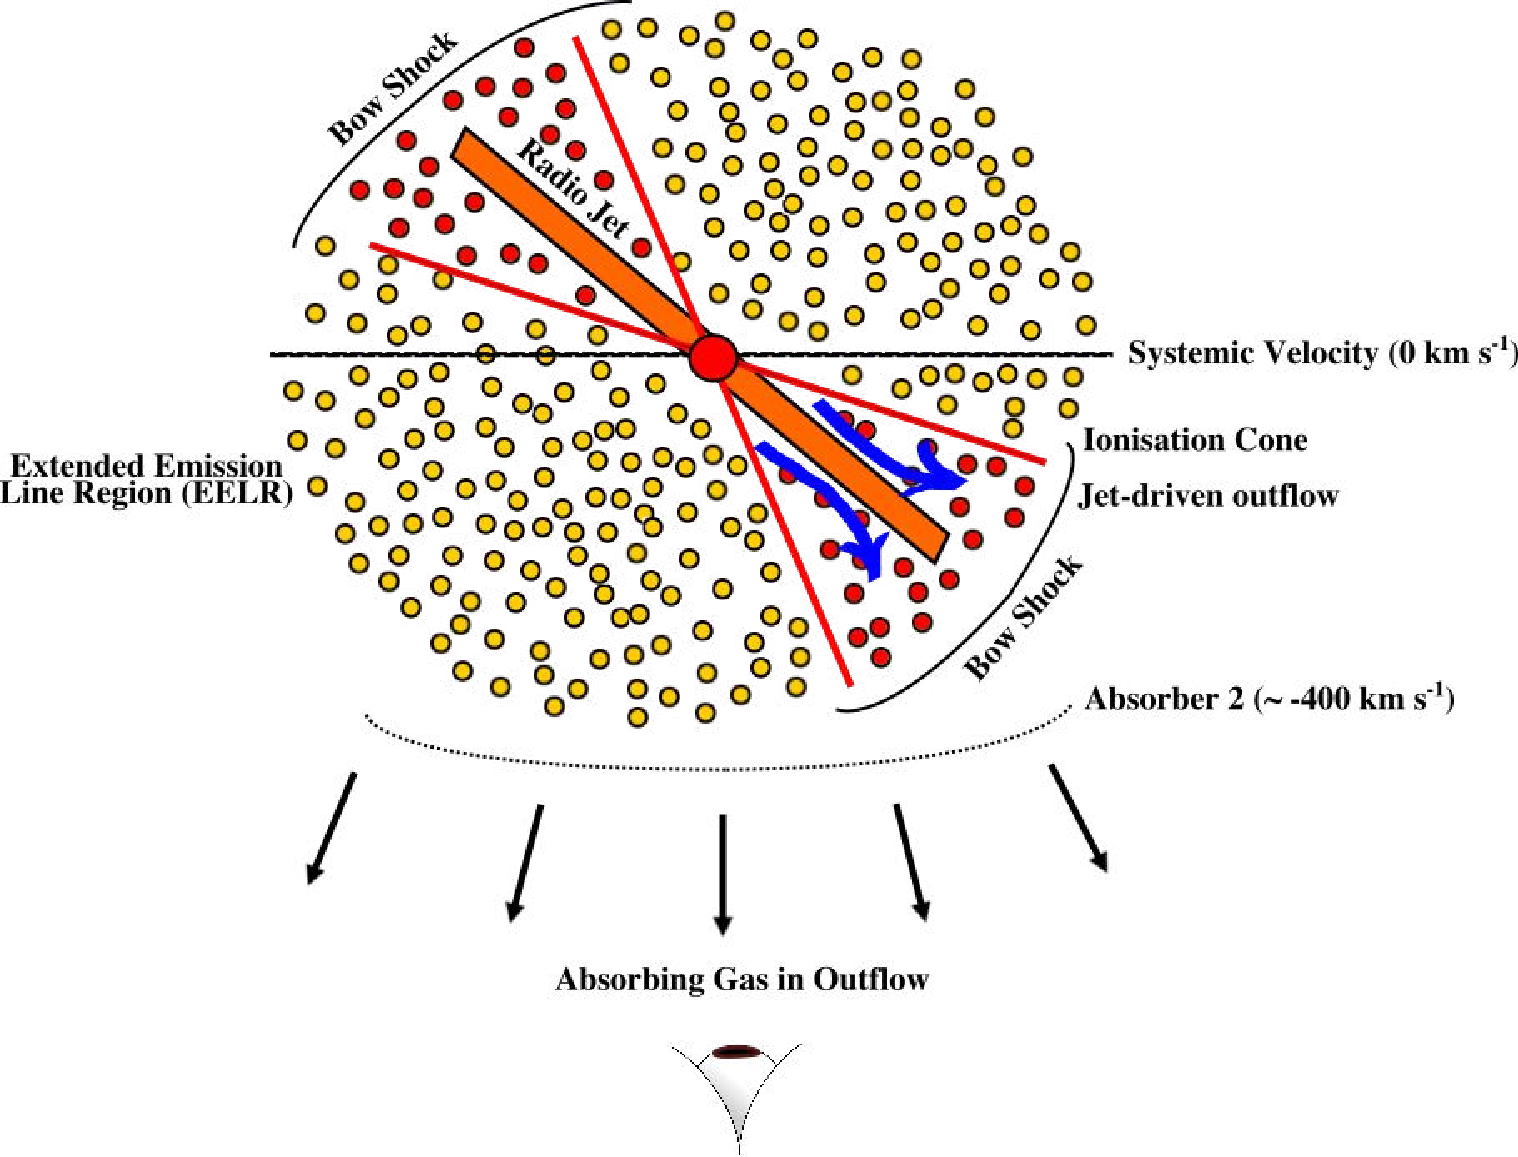
\includegraphics[width=0.8\textwidth]{plots_chp3/0943_absorption_schematic8.pdf}
\caption[Cross-section schematic of the circumgalactic medium of MRC 0943-242]{Cross-section schematic of the circumgalactic medium of Yggdrasil based on evidence from the MUSE data and previous measures. The gas has no defined spatial boundaries because its estimated size of d $\gtrsim$ 60 kpc is merely a minimum. The strong absorber screens emission that originates from the T $\simeq10^4-10^6$ K EELR gas (in yellow), comprising an extended region of ionised gas as well as gas that is directly ionised by the AGN ionisation cone (in red). The absorbing gas (shown as dotted curve) is also metal enriched, as shown by \ion{C}{IV}, \ion{N}{V,} and \ion{Si}{IV} that are detected at the same velocities as the \lya~absorption. The blueshifted component detected in \lya~and \ion{He}{II} is a jet-induced outflow (blue arrows). This outflowing, ionised, and turbulent gas is spatially offset from the HSBR of the halo, which implies that the radio jet is tilted relative to the projected plane. The location of absorber 2 is at a line-of-sight projected distance, which is dependent on the ionisation parameter, $U(r).$}
\label{fig:absorption-cartoon}
\end{figure}

The distance between the AGN and the absorbing gas can be estimated but is dependent on n$_{\ion{H}{I}}.$ Given that we cannot constrain the hydrogen density, we have only the ratio of ionisation parameters to infer the distance ratios of two absorbers, for instance, $r_2 / r_1 = \sqrt{U_1 / U_2}.$ Assuming that the \ion{H}{I} gas volume density of n$_\ion{H}{I} = 100$ cm$^{-3}$ is correct, we can approximate the distance of absorber 2 from the AGN using the integrated infrared luminosity, $L_{\rm IR}^{\rm AGN},$ of the host galaxy computed by \citet{falkendal2019}. According to Fig. \ref{fig:cloudy-abs2}, the ionisation parameter for absorber 2 is approximately $U \simeq 10^{-2.25}.$ Expressing the ionisation parameter as $U(r) = L/n_\ion{H}{I}r^2$ \citep[e.g.][]{rozanska2014}, we obtain a distance of $d \simeq 68^{+17}_{-14}$ kpc between absorber 2 and the AGN.

%---------------------------------------------------------------------------------------------------------------------------------------------------

\section{Discussion}\label{section:discussion}
\subsection{Blueshifted emission: companion galaxy or outflow?}\label{discussion:blueshifted-emission}

There is sufficient evidence to suggest that the preferred environments of radio galaxies are rich clusters and groups. This is at low redshifts (z $\lesssim$ 1), where the most radio-loud sources have a higher likelihood of residing in Mpc-scale overdense structures \citep[e.g.][]{best2007,karouzos2014a,magliocchetti2018,kolwa2019a}. Radio-loud sources are also prevalent in over-dense environments consisting of dusty starburst galaxies and/or \lya~emitters at z $>$ 1.2 \citep[e.g.][]{hatch2011,wylezalek2013,dannerbauer2014,saito2015}. Based on these findings, we hypothesise that the blueshifted emission in this source may stem from a proto-galaxy or dwarf satellite.

A well-studied example is a Minkowski's object, associated with the radio galaxy PKS 0123-016, which has an increased SFR due to the passage of the radio source's jets \citep{vanbreugel1985}. The high-velocity dispersions of the blueshifted emission in Yggdrasil imply a different origin of the gas. Only an AGN would produce the turbulent gas motions that can broaden lines such as \ion{He}{II} to line widths of FWHM=1500 km s$^{-1}.$ Furthermore, dwarf galaxies tend to have outflow velocities of ionised gas of $\varv_{\rm out} \lesssim 100$ km s$^{-1}$ \citep{martin2005}. Such velocities are well below the outflow rates we observe in the blueshifted ionised gas, where the velocities are $\varv_{\rm out} \gtrsim 400$ km s$^{-1}$. 

It is more likely that the gas turbulence is driven by the jets. This is also a known occurrence within the gas haloes of powerful radio galaxies \citep[e.g.][]{humphrey2006,morais2017,nesvadba2017a}. The jet-driven outflow scenario is well supported in 4.7 GHz radio observations that indicate from rotation measures that radio emission from the western radio lobe in this source propagates over a shorter path length than radio emission from the eastern lobe \citep[e.g.][]{carilli1997}. 

This configuration implies that the radio axis is also tilted at a non-zero inclination angle with respect to the projected plane, as shown Fig. \ref{fig:absorption-cartoon}. If the jets were parallel to the plane of the sky, we would observe similar rotation measures at both the east and west radio lobes. The rotation measure at the eastern lobe is higher than that at the western lobe. This jet inclination can also explain that the blueshifted emission is an outflow.

%It represents AGN photoionised outflowing gas that is jet-driven or perturbed as has been identified by \citet{villar-martin2003}. In that work, the high-surface brightness \ion{He}{II} emission was measured with line widths of FWHM $\sim$ 1600 km s$^{-1},$ which indicates perturbed gas kinematics in the extended emission line region (EELR). The perturbed emitting gas is also seen to have a close alignment with the radio jet axis as has been observed for several other HzRGs \citep[e.g.,][]{vanojik1996,humphrey2006}. 

The kinematics surrounding the jet-gas interactions in the gas halo of Yggdrasil have been measured in previous studies. \citet{villar-martin2003} reported that the narrow components of \ion{He}{II} emission were blueshifted from the systemic at velocity shifts of $\Delta \varv \sim$ 100 km s$^{-1}.$ This kinematically quiet component identified as having a FWHM $\sim$ 500 km s$^{-1}$ is shown to extend across the entire halo, well beyond the radio hotspot. This suggests jet-gas interactions. In addition to this, \citet{humphrey2006} found that the \ion{He}{II} gas that has a perturbed component with FWHM = 1760 km s$^{-1}$ and the quiescent component with FWHM = 750 km s$^{-1},$ respectively, at a velocity shift of $\Delta \varv \sim$ -250 km s$^{-1}$ is low-ionisation gas. We here find that the blueshifted emission has FWHM = 970 km s$^{-1}$ at $\Delta \varv \sim$ -1000 km s$^{-1}.$ Although our measured velocity shifts differ slightly from those of previous works, the common thread is that the \ion{He}{II} emission is blueshifted relative to systemic and aligned with the radio axis. This indicates jet-gas interactions.  

This view agrees well with observations from G16, who reported direct evidence for the ionisation cone to be projected along the radio jet axis in the form of extended \ion{He}{II}, \ion{C}{IV} and \ion{C}{III]} emission to the south-west of the source. A detailed discussion of the ionised gas kinematics is presented in S18. Their interpretation differs from ours only slightly in that our radio axis is tilted relative to the projected plane. 

In addition to \ion{He}{II} enhancement, a dust continuum and enhanced SFRs have been observed to the south-west of the inferred centre of the galaxy halo. G16 reported that the strong dust continuum may be a result of starbursts. This is supported by the SFR, which is measured to be  41 M$_\odot$ yr$^{-1}$  in Yggdrasil compared to  747 M$_\odot$ yr$^{-1} $ in the dusty regions in the south-west or companion sources \citep{falkendal2019}. Anti-correlations between radio size and 1.1 mm luminosities (that trace SF) measured from a sample of 16 HzRGs in \citet{humphrey2011} have explained why more evolved sources, such as Yggdrasil, have experienced a decline in their star formation. 

Furthermore, at z $>$ 3.0, metal enrichment and disturbed kinematics of extended gas haloes have been linked to jet-induced star formation in HzRGs \citep[e.g.][]{reuland2007}. It is not possible to state that there is jet-induced star-formation in this galaxy, however, because the projected radio size of $d \simeq 29$ kpc shows that the radio emission has not propagated far enough to induce star-formation at $d=65$ and 80 kpc from the host galaxy where the companion sources are located (G16).

\subsection{Possible origins and the nature of the absorbing gas}

We have shown that resonant line scattering or absorption of \ion{C}{IV}, \ion{N}{V,} and \ion{Si}{IV} photons occurs at the same velocities as do the line scattering or absorption of the strong \lya~absorber (absorber 2). Because of the uncertainties in measuring \ion{Si}{IV} absorption, we only discuss the main absorber around Ly$\alpha,$ \ion{N}{V,} and \ion{C}{IV.}  We obtained redshifts, column densities, and Doppler parameters for absorbers in the \lya~profile and found that the \ion{H}{I} column densities we measured are consistent with previous results (\citealp{vanojik1997,jarvis2003,wilman2004}; G16; S18). 

The formation of absorber 2 is well supported by simulations in which the neutral gas column is formed at the bow shock of radio jets and cools to T $\sim10^4-10^6$ K before fragmenting due to Rayleigh-Taylor (RT) instabilities that are brought about by the radio cocoon \citep{krause2002,krause2005}. S18 also showed that absorber 2 may be outflowing, which is in agreement with this framework. In addition to the high column density absorber, we also observed three \ion{H}{I} absorbers with column densities of $N_\ion{H}{I} = 10^{13}-10^{14}$ cm$^{-2}.$ The weak absorbers (absorbers 1, 3, and 4) could be fragmented shells of gas that have been disrupted by RT instabilities, hence their low column densities. In this scenario, the absorbers are formed through the ageing of the radio source \citep{wilman2004,binette2006}. 

Absorber 2 has a much higher \ion{H}{I} column density of $N_\ion{H}{I}/{\rm cm}^{-2} = 10^{19.2}.$ It may be a metal-poor gas shell that was expelled from the galaxy by an early AGN-related feedback event \citep{jarvis2003,binette2006}. We agree with this interpretation given both the strength of the absorber and the sum of its ionised and neutral mass, $M_{\rm T}/\rm{M}_\odot \geq 5.7\e{9},$ which is an order of magnitude lower than the stellar mass component of $M_*/\rm{M}_\odot = 1.2\e{11}$ of the galaxy, implying that a very energetic event would have to be responsible for expelling such a vast amount of gas. 

The nitrogen abundance of absorber 2, if photoionised primarily by the AGN, is in excess by a factor of 10 compared to its solar abundance. Because absorber 2 has a low metallicity overall, it may be nitrogen enhanced as a result of stellar winds. Chemically enriched gas from the ISM may have been swept up by stellar winds and progressively diluted the outflowing gas shell. 

This scenario is similar to that of the z = 3.09 star-forming galaxy of \citet{wilman2005}, which also contains an emission line region that is covered by a neutral gas shell of \ion{H}{I} column density, $N_\ion{H}{I}/{\rm cm}^{-2} \simeq 10^{19}$. The main difference between this source and ours is the SFR, which is much higher in the star-forming galaxy. If the mechanism by which the strong absorber in Yggdrasil has been enriched is a starburst-driven super-wind, it could mean that this process occurred at an earlier epoch, and we now observe the galaxy after a major starburst period has ceased. 

%---------------------------------------------------------------------------------------------------------------------------------------------------
\section{Summary}\label{section:summary}

%mention current episode of AGN activity results in photoionisation of the absorber but previous feedback activity formed it

We have examined the absorbing gas surrounding the host galaxy of  MRC 0943-242, Yggdrasil, using MUSE data. Our results prove that the \ion{H}{I} absorbers measured from the \lya~line are at the same velocities as the \ion{C}{IV} and \ion{N}{V} absorbers. The new integral field unit (IFU) dataset shows that the high \ion{H}{I} column density absorbing gas (\lya~absorber 2) with $N_\ion{H}{I}/{\rm cm}^{-2} = 10^{19.2}$  is a non-isotropic gas medium extending outwards from $r \gtrsim$ 60 kpc. It has a hydrogen fraction of X$_\ion{H}{I} \gtrsim 0.8,$ which makes it a predominantly ionised cloud with a total estimated mass of the neutral and  ionised gas of $M/\rm{M}_\odot \geq 5.7\e{9}.$ Detections of \ion{Si}{II} absorption at the same velocity as this absorber suggest that it is ionisation bounded.

Similar to previous studies, we observe a diffuse extension of \ion{He}{II} gas in alignment with the VLA-detected radio axis and the {\it HST} -detected optical/UV broad-band emission. The ionised gas is interpreted as a jet-induced outflow. The combination of radio axis and the observed \ion{He}{II} emission in this IFU data indicates that the radio jet is tilted at a non-zero inclination angle. This finding is well supported by rotation measures in the eastern and western radio lobes of the galaxy, which indicate that the emission from the eastern radio lobe has travelled farther along the line of sight than that emitted from the western lobe.

We also estimated the locations of the absorbers within the halo, assuming that they are outflowing. It is likely that absorber 2 is located at a greater distance from the AGN than absorber 1. Furthermore, the measured absorber  column densities in Yggdrasil are similar in magnitude to those of absorbers at velocity shifts of $\lvert \Delta \varv \rvert < 5000$ km s$^{-1}$ from quasars. 

Photoionisation models of the absorbing gas in \pkg{cloudy} have shown that ionising radiation from the AGN (for which we assumed a spectral energy distribution with a power-law shape of $\alpha=-1$) is capable of producing the \ion{C}{IV} and \ion{N}{V} column densities observed in absorber 2 when the gas has a metallicity of Z/Z$_\odot = 0.01$ in which the nitrogen abundance is enhanced by a factor of 10 relative to the solar abundance (i.e. N/C = 10). This high column density absorber is interpreted as primordial gas that was propelled outwards by an earlier feedback event (possibly an AGN). The gas has subsequently been ionised by an episode of AGN activity and chemical enriched through stellar winds. 

In conclusion, we showed the potential use of wide-field IFU instruments in understanding  the configuration of complex systems such as the haloes of HzRGs. Similar future analyses will be fundamental in unveiling the different gas structures surrounding HzRGs, ultimately adding important constraints on the physics of these objects.

%---------------------------------------------------------------------------------------------------------------------------------------------------
\section*{Acknowledgements}
SK acknowledges the International Max Planck Research School (IMPRS) on Astrophysics at Ludwig-Maximilians University (LMU) of Munich as well as the European Southern Observatory (ESO). All authors acknowledge the ESO Paranal Observatory as the source for VLT/MUSE data that formed the basis of this work. SK, CDB and JV thank Richard Wilman and Matt J. Jarvis for the ancillary UVES spectrum. We thank Paola Caselli and Ian Smail for providing helpful guidance and suggestions. SK thanks Marios Chatzikos and Fran Guzm{\'a}n for support with \pkg{cloudy}.  
  
This study has made use of data from the European Space Agency (ESA) mission
{\it Gaia} (\url{https://www.cosmos.esa.int/gaia}), processed by the {\it Gaia}
Data Processing and Analysis Consortium (DPAC,
\url{https://www.cosmos.esa.int/web/gaia/dpac/consortium}). Funding for the DPAC
has been provided by national institutions, in particular the institutions
participating in the {\it Gaia} Multilateral Agreement.

This work is on observations collected at the European Southern Observatory under ESO programmes 096.B-0752(A) and 068.B-0086(A). It is also based on observations made with the NASA/ESA Hubble Space Telescope, and obtained from the Hubble Legacy Archive, which is a collaboration between the Space Telescope Science Institute (STScI/NASA), the Space Telescope European Coordinating Facility (ST-ECF/ESA) and the Canadian Astronomy Data Centre (CADC/NRC/CSA).

MVM acknowledges support from the Spanish Ministerio de Ciencia, Innovación y Universidades (former Ministerio de Econom\'\i a y Competitividad) through the grant AYA2015-64346-C2-2-P. AH acknowledges FCT Fellowship SFRH/BPD/107919/2015; Support from
European Community Programme (FP7/2007-2013) under grant agreement
No. PIRSES-GA-2013-612701 (SELGIFS); Support from FCT through national funds (PTDC/FIS-AST/3214/2012 and UID/FIS/04434/2013), and by FEDER through COMPETE (FCOMP-01-0124-FEDER-029170) and COMPETE2020 
(POCI-01-0145-FEDER-007672). 

AH acknowledges support from the FCT-CAPES Transnational Cooperation Project "Parceria
Estrat\'egica em Astrof\'{i}sica Portugal-Brasil".
